
\documentclass[10pt,openany,a4paper]{article}
\usepackage{tikz, pgfplots, tkz-euclide,calc}
\usetikzlibrary{patterns,shapes.arrows,calc}
\usepackage{fancyhdr}
\usepackage{enumerate,enumitem}
\usepackage{cancel}
\usepackage{varwidth}

% TAMBAHKAN PACKAGE SENDIRI KALAU KURANG

\usepackage{geometry}
\geometry{
	left = 22mm,
	right = 22mm,
	top = 25mm,
	bottom = 25mm,
}
\usepackage{graphicx}
\usepackage{subcaption}
\usepackage{soul}
\usepackage{hyperref}
\usepackage{float}
\usepackage{setspace}
\usepackage{afterpage}
\usepackage{xcolor}
\usepackage[nosectionbib]{apacite}
\usepackage{lmodern}
\usepackage{mathtools}
\usepackage{upgreek}
\usepackage{siunitx}
% \usepackage{fontawesome5}
\usepackage{fontawesome6}
\usepackage{physics}
\usepackage{pdfpages}
\usepackage{hyperref}
\renewcommand{\baselinestretch}{1.3}
\usepackage{multicol}
\usepackage{hyperref,ragged2e,amsmath,multicol,gensymb,setspace,
fancyhdr,amsfonts,tikz,pgfplots,nccmath,enumerate,verbatim,amsthm,physics}
\usepgfplotslibrary{polar,fillbetween}
% Disable tikz externalization to avoid requiring -shell-escape
\usepgfplotslibrary{external}
\tikzexternalize[prefix=tikz/]
\tikzset{reuse path/.code={\pgfsyssoftpath@setcurrentpath{#1}}}
\usetikzlibrary{shapes.geometric,arrows}
\newcommand\mylog[1]{\mathop{{}^{#1}\mathrm{log}}}
\pgfplotsset{compat=1.15}
\pgfplotsset{my style/.append style={axis x line=middle, axis y line=
middle, xlabel={$x$}, ylabel={$y$}, axis equal }}
\usepackage{etoolbox}
% remove stray \makeatother
\newtheorem{defn}{Definisi}[section]
\newtheorem{teo}[defn]{Teorema}
\newtheorem{thm}{Teorema}[section]
\newtheorem{lemma}{Lemma}
\newtheorem{lemmas}[defn]{Lemma}
\newtheorem{cor}[defn]{Akibat}
\newtheorem{asumsi}[defn]{Asumsi}
\theoremstyle{definition}
\newtheorem{con}{Contoh}[section]
\theoremstyle{definition}
\theoremstyle{plain}
\newtheorem{prop}{Proposisi}[section]
\renewcommand{\proofname}{Bukti}
\renewcommand{\thethm}{\arabic{chapter}.\arabic{thm}}

\newcommand{\normlp}[1]{\left\|#1\right\|_{L^p_{\lambda}(0,T;H)}}% Fungsi norm (||x||)
\newcommand{\R}{\mathbb{R}}
\renewcommand{\natural}{\mathbb{N}}
\newcommand{\Xpl}{X^R_{p,\lambda}}
\newcommand{\Xpls}{X^R_{p,\lambda^*}}
\newcommand{\qpl}{q^R_{p,\lambda}}
\newcommand{\qpls}{q^R_{p,\lambda^*}}
\pagestyle{fancy}
\fancyhf{}
\lhead{Halaman \thepage}
% \cfoot{\faXTwitter\ \href{https://x.com/ahmadzakiyudin_/}{@ahmadzakiyudin\_} | \faInstagram\ \href{https://instagram.com/ahmadzakiyudin_/}{@ahmadzakiyudin\_} | \faTiktok\ \href{https://tiktok.com/@ahmathz/}{@ahmathz}}
% \rhead{Pembahasan Soal ETS \\ Kalkulus 1 ITS 2025/2026}
\hypersetup{
    colorlinks=true,
    linkcolor=blue,
    filecolor=blue,      
    urlcolor=blue,
}
\newenvironment{jawab}[2][tes]{%
% \fbox{\begin{minipage}{14.65cm}
% \par + \noindent: selalu mulai di baris baru tanpa menjorok,
% termasuk setelah display math (align, \[ \]) di akhir soal
\par\noindent\textbf{Kata kunci materi:} #1.\\
\textbf{Penyelesaian:} #2%
% \end{minipage}}
}{}

\newenvironment{jawab2}[2][tes]{
\fbox{\begin{minipage}{14.65cm}
 #2
\end{minipage}}}{}

\newenvironment{jawaban}[2][tes]{
\colorlet{oldcolor}{.}
        \color{red}
        \setlength{\fboxrule}{1pt}\boxed{\color{oldcolor}#2}\color{oldcolor}.
}{}

\newenvironment{jawaban2}[2][tes]{
\colorlet{oldcolor}{.}
        \color{red}
        \setlength{\fboxrule}{1pt}\fbox{\color{oldcolor}#2}\color{oldcolor}.
}{}

\newenvironment{penting}[2][tes]{
\colorlet{oldcolor}{.}
\color{blue}
\fbox{\color{oldcolor}#2}\color{oldcolor}
}{}

\begin{document}
% \begin{titlepage}
%     \vspace*{\fill}
%     \begin{center}
%       \Huge {PEMBAHASAN SOAL EAS \\ KALKULUS II \\ TAHUN 2024/2025}\\[0.4 cm]
%       \huge {Ahmad Hisbu Zakiyudin}\\[0.2 cm]
%       \Large {(\href{https://instagram.com/ahmadzakiyudin_/}{@ahmadzakiyudin\_})}
%     \end{center}
%     \vspace*{\fill}
%   \end{titlepage}
% !TEX root = ../../BookTemplate.tex
%%%%%%%%%%%%%%%%%%%%%%%%%%%%%%%%%%%%%%%%%%%%%%%%%%%%%%%%%%%%%%%%%%%%%%%%%%%%%%%%%%
% \begin{titlepage}
%     \raggedleft	
% 	\hspace{.025\textwidth}
% 	\parbox[b]{\textwidth}{
%     \vspace{1.5cm}
% 		{\Huge\bfseries Pembahasan Soal EAS}                \\[20pt]
% 		{\huge\textit\ Kalkulus II}\\ \\[10pt]
%         {\Large\textsc{Tahun 2024/2025}}}
% \vfill
% \rule{1pt}{.14\textheight}
% \hspace{.025\textwidth}
%     \raisebox{10pt}{\parbox[b]{.95\textwidth}{ 
%         {\Large\textsc{Ahmad Hisbu Zakiyudin}}              \\[10pt]
%         \large{\href{https://instagram.com/ahmadzakiyudin_/}{@ahmadzakiyudin\_}}               \\[25pt]
%         {\large 5 Juni 2026}}}
% \end{titlepage}
\begin{titlepage}
	\centering % Center everything on the title page
	% \scshape % Use small caps for all text on the title page
	\vspace*{1.5\baselineskip} % White space at the top of the page
% ===================
%	Title Section 	
% ===================

	\rule{13cm}{1.6pt}\vspace*{-\baselineskip}\vspace*{2pt} % Thick horizontal rule
	\rule{13cm}{0.4pt} % Thin horizontal rule
	
		\vspace{0.75\baselineskip} % Whitespace above the title
% ========== Title ===============	
	{	\Huge Pembahasan Soal\\ 
			\vspace{4mm}
		Tryout ETS Kalkulus 1 \\ \vspace{2mm} \huge{Tahun 2026/2027}\\	}
% ======================================
		\vspace{0.75\baselineskip} % Whitespace below the title
	\rule{13cm}{0.4pt}\vspace*{-\baselineskip}\vspace{3.2pt} % Thin horizontal rule
	\rule{13cm}{1.6pt} % Thick horizontal rule
	
		\vspace{1.75\baselineskip} % Whitespace after the title block
% =================
%	Information	
% =================
{\large Oleh: Ahmad Hisbu Zakiyudin}
	% {\large Oleh: Ahmad Hisbu Zakiyudin \\
	% 	\vspace*{1.2\baselineskip}
	% \href{https://instagram.com/ahmadzakiyudin_/}{@ahmadzakiyudin\_}} \\
	\vfill
	\vspace{1mm}
\huge{Selamat Belajar!}
\end{titlepage}
\makeatletter
\setlength\fboxsep{3pt}
% ensure enough header height for fancyhdr
\setlength{\headheight}{24pt}
% Kop tiap kelompok: #1 kelompok, #2 kelas, #3 departemen, #4 jadwal kuliah, #5 sesi
\newcommand{\kopsoal}[5]{%
 \begin{center}
	{\underline{\textbf{\MakeUppercase{Soal dan Pembahasan Tryout ETS Kalkulus 1 Tahun 2026/2027}}}}
    \end{center}

    \begin{center}
	\begin{tabular}{lcl}
		Mata kuliah/SKS & : & Kalkulus 1 ( SM234101 ) / 3 SKS\\
		Kelompok & : & #1\\
		Kelas & : & #2\\
		Departemen & : & #3\\
		Jadwal kuliah & : & #4\\
		Sesi & : & #5\\
		Waktu & : & 100 menit\\
		Sifat & : & Tertutup\\
  ~
	\end{tabular}

    \noindent\rule{\textwidth}{2.pt}
        \end{center}}

% Kop kelompok IUP (bahasa Inggris): #1 kelompok, #2 kelas, #3 departemen, #4 jadwal kuliah, #5 sesi
\newcommand{\kopsoaliup}[5]{%
 \begin{center}
	{\underline{\textbf{\MakeUppercase{Soal dan Pembahasan Tryout ETS Kalkulus 1 Tahun 2026/2027}}}}
    \end{center}

    \begin{center}
	\begin{tabular}{lcl}
		Course / Credit & : & Kalkulus 1 ( SM234101 ) / 3 SKS\\
		Group & : & #1\\
		Class & : & #2\\
		Department & : & #3\\
		Lecture schedule & : & #4\\
		Session & : & #5\\
		Time & : & 100 minutes\\
		Type & : & Closed\\
  ~
	\end{tabular}

    \noindent\rule{\textwidth}{2.pt}
        \end{center}}

% Kop tryout Matematika 2 SKS: #1 kelompok, #2 kelas, #3 departemen, #4 jadwal kuliah, #5 sesi
\newcommand{\kopsoalmat}[5]{%
 \begin{center}
	{\underline{\textbf{\MakeUppercase{Soal dan Pembahasan Tryout ETS Matematika Tahun 2026/2027}}}}
    \end{center}

    \begin{center}
	\begin{tabular}{lcl}
		Mata kuliah/SKS & : & Matematika ( SM234152 ) / 2 SKS\\
		Kelompok & : & #1\\
		Kelas & : & #2\\
		Departemen & : & #3\\
		Jadwal kuliah & : & #4\\
		Sesi & : & #5\\
		Waktu & : & 100 menit\\
		Sifat & : & Tertutup\\
  ~
	\end{tabular}

    \noindent\rule{\textwidth}{2.pt}
        \end{center}}

% Kop tryout Matematika 2 SKS IUP (bahasa Inggris)
\newcommand{\kopsoalmatiup}[5]{%
 \begin{center}
	{\underline{\textbf{\MakeUppercase{Soal dan Pembahasan Tryout ETS Matematika Tahun 2026/2027}}}}
    \end{center}

    \begin{center}
	\begin{tabular}{lcl}
		Course / Credit & : & Matematika ( SM234152 ) / 2 SKS\\
		Group & : & #1\\
		Class & : & #2\\
		Department & : & #3\\
		Lecture schedule & : & #4\\
		Session & : & #5\\
		Time & : & 100 minutes\\
		Type & : & Closed\\
  ~
	\end{tabular}

    \noindent\rule{\textwidth}{2.pt}
        \end{center}}


%%%%%%%%%%%%%%%%%%%%%%%%%%%%%%%%%%%%%%%%%%%%%%%%%%%%%%%%%%%%%%%%%%%%%%%%%%%%%%
% Kal-5
\kopsoal{Kal-5}{22-27}{T. Fisika, T. Material dan Metalurgi, Rkp}{Senin, Rabu; 07.00-09.30}{1}
\begin{enumerate}
    \item Dapatkan himpunan penyelesaian pertidaksamaan
    \begin{align*}
        3\leq\frac{x^2+2}{x}<x+2
    \end{align*}
    \begin{jawab}[pertidaksamaan rasional, pertidaksamaan ganda, garis bilangan, irisan himpunan]{~\\
        Pertidaksamaan ganda tersebut dapat dipecah menjadi dua pertidaksamaan yang harus dipenuhi sekaligus, yaitu
        \begin{align*}
            \colorlet{oldcolor}{.}
        \color{blue}
        \setlength{\fboxrule}{1pt} \boxed{\color{oldcolor}3\leq\frac{x^2+2}{x}}\color{oldcolor} \quad\text{dan}\quad \colorlet{oldcolor}{.}
        \color{blue}
        \setlength{\fboxrule}{1pt} \boxed{\color{oldcolor}\frac{x^2+2}{x}<x+2}\color{oldcolor}.
        \end{align*}
        Diperhatikan bahwa $x\neq 0$ karena $x$ berada pada penyebut.
        \begin{enumerate}
            \item[(i)] Untuk $3\leq\frac{x^2+2}{x}$, pindahkan semua suku ke ruas kiri sehingga ruas kanan bernilai nol:
            \begin{align*}
                \frac{x^2+2}{x}-3 &\geq 0\\
                \frac{x^2+2-3x}{x} &\geq 0\\
                \frac{(x-1)(x-2)}{x} &\geq 0.
            \end{align*}
            Pembuat nolnya adalah $x=0$, $x=1$, dan $x=2$. Dengan uji titik, misalkan $x=-1$ diperoleh $\frac{(-2)(-3)}{-1}<0$, $x=\frac{1}{2}$ diperoleh $\frac{(-\frac{1}{2})(-\frac{3}{2})}{\frac{1}{2}}>0$, $x=\frac{3}{2}$ diperoleh $\frac{(\frac{1}{2})(-\frac{1}{2})}{\frac{3}{2}}<0$, dan $x=3$ diperoleh $\frac{(2)(1)}{3}>0$.
            \begin{center}
                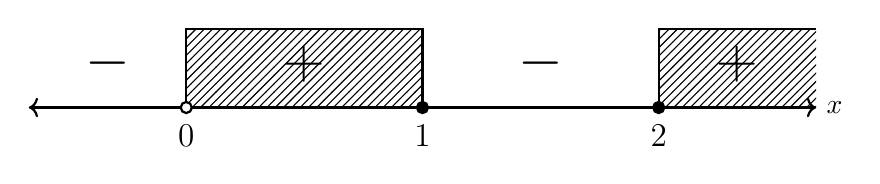
\begin{tikzpicture}
    \draw[thick,<->] (-5,0) -- (5,0) node[right] {$x$};
    \fill[pattern=north east lines] (-3,0) rectangle (0,1);
    \fill[pattern=north east lines] (3,0) rectangle (5,1);
    \draw[thick] (-3,0) -- (-3,1) -- (0,1) -- (0,0);
    \draw[thick] (3,0) -- (3,1) -- (5,1);
    \draw (-3,-0.1) node[below] {\large{$0$}};
    \draw (0,-0.1) node[below] {\large{$1$}};
    \draw (3,-0.1) node[below] {\large{$2$}};
    \draw (-4,0.2) node[above] {\huge{$-$}};
    \draw (-1.5,0.2) node[above] {\huge{$+$}};
    \draw (1.5,0.2) node[above] {\huge{$-$}};
    \draw (4,0.2) node[above] {\huge{$+$}};
    \draw[fill=white, thick] (-3,0) circle (2pt);
    \draw[fill=black, thick] (0,0) circle (2pt);
    \draw[fill=black, thick] (3,0) circle (2pt);
                \end{tikzpicture}
            \end{center}
            Karena yang diminta lebih dari atau sama dengan nol, diperoleh $\colorlet{oldcolor}{.}
        \color{blue}
        \setlength{\fboxrule}{1pt} \boxed{\color{oldcolor}HP_1=(0,1]\cup[2,\infty)}\color{oldcolor}$.
            \item[(ii)] Untuk $\frac{x^2+2}{x}<x+2$, dengan cara yang sama diperoleh
            \begin{align*}
                \frac{x^2+2}{x}-(x+2) &< 0\\
                \frac{x^2+2-x^2-2x}{x} &< 0\\
                \frac{2(1-x)}{x} &< 0.
            \end{align*}
            Pembuat nolnya adalah $x=0$ dan $x=1$. Dengan uji titik, misalkan $x=-1$ diperoleh $\frac{2(2)}{-1}<0$, $x=\frac{1}{2}$ diperoleh $\frac{2(\frac{1}{2})}{\frac{1}{2}}>0$, dan $x=2$ diperoleh $\frac{2(-1)}{2}<0$.
            \begin{center}
                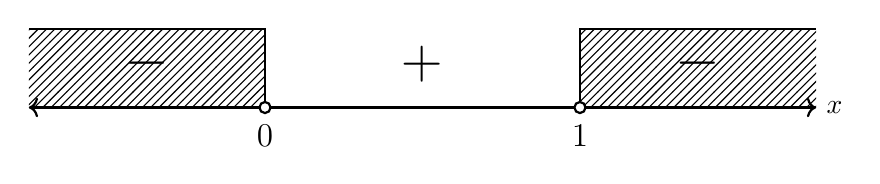
\begin{tikzpicture}
    \draw[thick,<->] (-5,0) -- (5,0) node[right] {$x$};
    \fill[pattern=north east lines] (-5,0) rectangle (-2,1);
    \fill[pattern=north east lines] (2,0) rectangle (5,1);
    \draw[thick] (-5,1) -- (-2,1) -- (-2,0);
    \draw[thick] (2,0) -- (2,1) -- (5,1);
    \draw (-2,-0.1) node[below] {\large{$0$}};
    \draw (2,-0.1) node[below] {\large{$1$}};
    \draw (-3.5,0.2) node[above] {\huge{$-$}};
    \draw (0,0.2) node[above] {\huge{$+$}};
    \draw (3.5,0.2) node[above] {\huge{$-$}};
    \draw[fill=white, thick] (-2,0) circle (2pt);
    \draw[fill=white, thick] (2,0) circle (2pt);
                \end{tikzpicture}
            \end{center}
            Karena yang diminta kurang dari nol, diperoleh $\colorlet{oldcolor}{.}
        \color{blue}
        \setlength{\fboxrule}{1pt} \boxed{\color{oldcolor}HP_2=(-\infty,0)\cup(1,\infty)}\color{oldcolor}$.
        \end{enumerate}
        Himpunan penyelesaian pertidaksamaan ganda adalah irisan dari kedua himpunan tersebut, yaitu
        \begin{align*}
            HP_1\cap HP_2 = \big((0,1]\cup[2,\infty)\big)\cap\big((-\infty,0)\cup(1,\infty)\big) = [2,\infty).
        \end{align*}
        Sebagai pengecekan, untuk $x=2$ diperoleh $\frac{4+2}{2}=3$, dan berlaku $3\leq 3<4$. Jadi himpunan penyelesaiannya adalah $\colorlet{oldcolor}{.}
        \color{red}
        \setlength{\fboxrule}{1pt} \boxed{\color{oldcolor}\{x\in\mathbb{R} : x\geq 2\}=[2,\infty)}\color{oldcolor}$.
    }
    \end{jawab}

    \item Diberikan fungsi $f(x)=\dfrac{1}{x+2}$ dan $g(x)=3-\sqrt{x}$.
    \begin{enumerate}
        \item Tentukan domain dari fungsi $f$ dan $g$.
        \item Dapatkan fungsi $(f\circ g)(x)$ beserta domainnya.
    \end{enumerate}
    \begin{jawab}[domain fungsi, fungsi komposisi, domain fungsi komposisi]{
        \begin{enumerate}
            \item Diperhatikan bahwa $f(x)$ merupakan fungsi rasional, sehingga domainnya adalah semua bilangan real kecuali nilai yang membuat penyebutnya sama dengan nol, yaitu $x+2\neq 0$. Jadi
            \[
            \colorlet{oldcolor}{.}
        \color{red}
        \setlength{\fboxrule}{1pt} \boxed{\color{oldcolor}D(f)=\{x \in \mathbb{R} : x \neq -2\}}\color{oldcolor}.
            \]
            Selanjutnya, diperhatikan bahwa $g(x)$ memuat akar kuadrat, sehingga domainnya adalah semua bilangan real yang membuat ekspresi di dalam akar kuadrat tak negatif. Jadi
            \[
            \colorlet{oldcolor}{.}
        \color{red}
        \setlength{\fboxrule}{1pt} \boxed{\color{oldcolor}D(g)=\{x \in \mathbb{R} : x \geq 0\}}\color{oldcolor}.
            \]
            \item Diperhatikan bahwa
            \begin{align*}
                (f\circ g)(x) = f(g(x)) = f(3 - \sqrt{x}) = \frac{1}{(3 - \sqrt{x}) + 2} = \colorlet{oldcolor}{.}
        \color{red}
        \setlength{\fboxrule}{1pt} \boxed{\color{oldcolor}\frac{1}{5 - \sqrt{x}}}\color{oldcolor}
            \end{align*}
            Domain dari fungsi komposisi $f\circ g$ adalah semua nilai $x$ pada domain $g$ sehingga nilai dari $g(x)$ berada pada domain $f$, yang dapat dirumuskan sebagai
            \begin{align*}
                \colorlet{oldcolor}{.}
        \color{blue}
        \setlength{\fboxrule}{1pt} \boxed{\color{oldcolor}D(f\circ g) = \{x \in D(g) : g(x) \in D(f)\} = \{x \in [0, \infty) : 3 - \sqrt{x} \neq -2\}}\color{oldcolor}.
            \end{align*}
            Karena $3 - \sqrt{x} = -2$ jika dan hanya jika $\sqrt{x} = 5$, yang berarti $x = 25$, didapatkan
            \begin{align*}
                \colorlet{oldcolor}{.}
        \color{red}
        \setlength{\fboxrule}{1pt} \boxed{\color{oldcolor}D(f\circ g) = [0, \infty) \setminus \{25\} = [0, 25) \cup (25, \infty)}\color{oldcolor}.
            \end{align*}
        \end{enumerate}
    }
    \end{jawab}

    \item Diberikan suatu fungsi $f(x)=1+\sqrt{4-x^2}$ dengan domain $f$ adalah $[a,2]$.
    \begin{enumerate}
        \item Tentukan nilai terkecil $a$ agar $f^{-1}(x)$ ada.
        \item Dapatkan $f^{-1}(x)$.
        \item Dapatkan domain dan range dari $f^{-1}(x)$.
    \end{enumerate}
    \begin{jawab}[fungsi satu-satu, setengah lingkaran, fungsi invers, domain dan range]{
        \begin{enumerate}
            \item Suatu fungsi mempunyai invers jika fungsi tersebut satu-satu (injektif). Diperhatikan bahwa jika $y=1+\sqrt{4-x^2}$, maka $y-1=\sqrt{4-x^2}\geq 0$ dan
            \begin{align*}
                (y-1)^2 = 4-x^2 \iff \colorlet{oldcolor}{.}
        \color{blue}
        \setlength{\fboxrule}{1pt} \boxed{\color{oldcolor}x^2+(y-1)^2=4}\color{oldcolor},\quad y\geq 1,
            \end{align*}
            sehingga grafik $f$ adalah setengah lingkaran bagian atas dengan pusat $(0,1)$ dan jari-jari $2$. Grafik ini naik pada $[-2,0]$ dan turun pada $[0,2]$, sehingga jika domainnya memuat titik di kiri dan kanan $x=0$, fungsi $f$ tidak satu-satu (misalnya $f(-1)=f(1)=1+\sqrt{3}$). Agar $f$ satu-satu pada $[a,2]$, haruslah $a\geq 0$. Jadi nilai terkecil $a$ adalah $\colorlet{oldcolor}{.}
        \color{red}
        \setlength{\fboxrule}{1pt} \boxed{\color{oldcolor}a=0}\color{oldcolor}$.
            \item Misalkan $y=f(x)$ dengan $x\in[0,2]$, kemudian selesaikan sehingga terbentuk $x$ dalam fungsi $y$. Diperoleh
            \begin{align*}
                y &= 1+\sqrt{4-x^2}\\
                y-1 &= \sqrt{4-x^2}\\
                (y-1)^2 &= 4-x^2\\
                x^2 &= 4-(y-1)^2\\
                x &= \sqrt{4-(y-1)^2} \quad (\text{karena } x\geq 0).
            \end{align*}
            Dari sini didapatkan $x = f^{-1}(y) = \sqrt{4-(y-1)^2}$. Dengan mengganti $y$ dengan $x$, diperoleh
            \begin{align*}
                \colorlet{oldcolor}{.}
        \color{red}
        \setlength{\fboxrule}{1pt} \boxed{\color{oldcolor}f^{-1}(x) = \sqrt{4-(x-1)^2} = \sqrt{3+2x-x^2}}\color{oldcolor}.
            \end{align*}
            \item Pada domain $[0,2]$, fungsi $f$ turun dari $f(0)=1+\sqrt{4}=3$ sampai $f(2)=1+\sqrt{0}=1$, sehingga range dari $f$ adalah $R(f)=[1,3]$. Domain dari fungsi invers adalah range dari fungsi asli dan range dari fungsi invers adalah domain dari fungsi asli, yaitu
            \begin{align*}
                \colorlet{oldcolor}{.}
        \color{red}
        \setlength{\fboxrule}{1pt} \boxed{\color{oldcolor}D(f^{-1}) = R(f) = [1, 3]}\color{oldcolor} \quad\text{dan}\quad \colorlet{oldcolor}{.}
        \color{red}
        \setlength{\fboxrule}{1pt} \boxed{\color{oldcolor}R(f^{-1}) = D(f) = [0, 2]}\color{oldcolor}.
            \end{align*}
        \end{enumerate}
    }
    \end{jawab}

    \item Diberikan fungsi $f(x)=\begin{cases}
        \dfrac{x^3-27}{3x-9}, & x\neq 3\\
        k, & x=3
    \end{cases}$.
    \begin{enumerate}
        \item Tentukan nilai $k$ sehingga $f(x)$ kontinu di $x=3$.
        \item Berdasarkan hasil dari (a), nyatakan $f(x)$ sebagai polinomial.
    \end{enumerate}
    \begin{jawab}[fungsi kontinu, limit, polinomial]{
        \begin{enumerate}
            \item Ingat kembali syarat fungsi kontinu di suatu titik \(x = a\) adalah
            \begin{enumerate}
                \item \(f(a)\) terdefinisi
                \item \(\displaystyle \lim_{x \to a} f(x)\) ada, yaitu $\displaystyle \lim_{x \to a^-} f(x) = \lim_{x \to a^+} f(x)$
                \item \(\displaystyle\lim_{x \to a} f(x) = f(a)\)
            \end{enumerate}
            Diperhatikan bahwa untuk \(x = 3\), \(\colorlet{oldcolor}{.}
        \color{blue}
        \setlength{\fboxrule}{1pt} \boxed{\color{oldcolor}f(3) = k~\text{terdefinisi}}\color{oldcolor}\). Karena limit di $x=3$ artinya nilai fungsi di sekitar $x=3$ tetapi $x\neq 3$, didapatkan limitnya adalah
            \begin{align*}
            \lim_{x \to 3} f(x) = \lim_{x \to 3} \frac{x^3 - 27}{3x - 9} = \lim_{x \to 3} \frac{(x-3)(x^2 + 3x + 9)}{3(x-3)} = \lim_{x \to 3} \frac{x^2 + 3x + 9}{3} = \frac{9 + 9 + 9}{3} = \colorlet{oldcolor}{.}
        \color{blue}
        \setlength{\fboxrule}{1pt} \boxed{\color{oldcolor}9}\color{oldcolor}.
            \end{align*}
            Selanjutnya, untuk syarat ketiga, haruslah $\displaystyle \colorlet{oldcolor}{.}
        \color{blue}
        \setlength{\fboxrule}{1pt} \boxed{\color{oldcolor}\lim_{x \to 3} f(x) = f(3)}\color{oldcolor}$, sehingga diperoleh $\colorlet{oldcolor}{.}
        \color{red}
        \setlength{\fboxrule}{1pt} \boxed{\color{oldcolor}k=9}\color{oldcolor}$.
        \item Diperhatikan bahwa untuk $x\neq 3$, berlaku
        \begin{align*}
            f(x) = \frac{x^3 - 27}{3x - 9} = \frac{(x-3)(x^2 + 3x + 9)}{3(x-3)} = \frac{x^2 + 3x + 9}{3} = \frac{1}{3}x^2 + x + 3.
        \end{align*}
        Untuk $x=3$, nilai polinomial tersebut adalah $\frac{1}{3}(9)+3+3=9=k$. Berdasarkan hasil dari (a), diperoleh bahwa \(f(x)\) kontinu di \(x=3\) jika \(k=9\). Dengan demikian, fungsi \(f(x)\) dapat dinyatakan sebagai polinomial
        \begin{align*}
            \colorlet{oldcolor}{.}
        \color{red}
        \setlength{\fboxrule}{1pt} \boxed{\color{oldcolor}f(x) = \frac{1}{3}x^2 + x + 3}\color{oldcolor}.
        \end{align*}
        \end{enumerate}
    }
    \end{jawab}

    \item Diberikan fungsi implisit $x^2+2y^2-3xy+2x-y=3$.
    \begin{enumerate}
        \item Tentukan $\dfrac{dy}{dx}$ di titik $(2,1)$.
        \item Dapatkan persamaan garis singgung kurva di titik tersebut.
    \end{enumerate}
    \begin{jawab}[diferensiasi implisit, aturan perkalian, aturan rantai, persamaan garis singgung]{
        \begin{enumerate}
            \item Kita turunkan kedua ruas persamaan terhadap $x$, dengan mengingat bahwa $y$ adalah fungsi dari $x$ (yaitu $y=y(x)$). Dengan aturan rantai, $\colorlet{oldcolor}{.}
        \color{blue}
        \setlength{\fboxrule}{1pt} \boxed{\color{oldcolor}\frac{d}{dx}(2y^2) = 4y\frac{dy}{dx}}\color{oldcolor}$, dan dengan aturan perkalian, $\colorlet{oldcolor}{.}
        \color{blue}
        \setlength{\fboxrule}{1pt} \boxed{\color{oldcolor}\frac{d}{dx}(3xy) = 3y + 3x\frac{dy}{dx}}\color{oldcolor}$. Diperoleh
            \begin{align*}
                \frac{d}{dx}(x^2) + \frac{d}{dx}(2y^2) - \frac{d}{dx}(3xy) + \frac{d}{dx}(2x) - \frac{d}{dx}(y) &= \frac{d}{dx}(3)\\
                2x + 4y\frac{dy}{dx} - 3y - 3x\frac{dy}{dx} + 2 - \frac{dy}{dx} &= 0.
            \end{align*}
            Selanjutnya, kumpulkan semua suku yang mengandung $\frac{dy}{dx}$ di satu ruas:
            \begin{align*}
                (4y - 3x - 1)\frac{dy}{dx} &= 3y - 2x - 2\\
                \frac{dy}{dx} &= \colorlet{oldcolor}{.}
        \color{blue}
        \setlength{\fboxrule}{1pt} \boxed{\color{oldcolor}\frac{3y - 2x - 2}{4y - 3x - 1}}\color{oldcolor}.
            \end{align*}
            Terlebih dahulu dicek bahwa titik $(2,1)$ terletak pada kurva, yaitu $2^2+2(1)^2-3(2)(1)+2(2)-1=4+2-6+4-1=3$. Selanjutnya, substitusi titik $(2,1)$ ke dalam turunan:
            \begin{align*}
                \frac{dy}{dx}\bigg|_{(2,1)} = \frac{3(1) - 2(2) - 2}{4(1) - 3(2) - 1} = \frac{-3}{-3} = \colorlet{oldcolor}{.}
        \color{red}
        \setlength{\fboxrule}{1pt} \boxed{\color{oldcolor}1}\color{oldcolor}.
            \end{align*}
            \item Gradien garis singgung di titik $(2,1)$ adalah $m=1$. Dengan menggunakan persamaan garis $y - y_1 = m(x - x_1)$, di mana $(x_1,y_1)=(2,1)$, diperoleh
            \begin{align*}
                y - 1 &= 1(x - 2)\\
                y &= x - 1.
            \end{align*}
            Jadi persamaan garis singgung di titik $(2,1)$ adalah $\colorlet{oldcolor}{.}
        \color{red}
        \setlength{\fboxrule}{1pt} \boxed{\color{oldcolor}y = x - 1}\color{oldcolor}$.
        \end{enumerate}
    }
    \end{jawab}
\end{enumerate}

\newpage

%%%%%%%%%%%%%%%%%%%%%%%%%%%%%%%%%%%%%%%%%%%%%%%%%%%%%%%%%%%%%%%%%%%%%%%%%%%%%%
% Kal-6
\kopsoal{Kal-6}{28-31}{T. Perkapalan, T. Transportasi Laut, T. Bangunan Lepas Pantai}{Senin, Rabu; 07.00-09.30}{1}
\begin{enumerate}
    \item Diketahui garis $g_1: y=-2x+8$ dan garis $g_2: y=x+2$.
    \begin{enumerate}
        \item Tentukan titik potong kedua garis $g_1$ dan $g_2$.
        \item Tentukan titik potong $g_1$ dan $g_2$ masing-masing dengan garis $x=4$.
        \item Gambarkan sketsa ketiga garis $g_1$, $g_2$, dan garis $x=4$. Hitung luas segitiga yang dibentuk ketiga garis tersebut.
    \end{enumerate}
    \begin{jawab}[persamaan garis, titik potong garis, luas segitiga]{
        \begin{enumerate}
            \item Untuk menentukan titik potong kedua garis, kita samakan persamaan kedua garis, yaitu $-2x+8=x+2$, sehingga $6=3x$, dan diperoleh $x=2$. Selanjutnya, substitusi \(x = 2\) ke dalam salah satu persamaan garis, misalkan \(g_2\), diperoleh $y=2+2=4$. Jadi titik potong kedua garis adalah \(\colorlet{oldcolor}{.}
        \color{red}
        \setlength{\fboxrule}{1pt} \boxed{\color{oldcolor}(2,4)}\color{oldcolor}\), misalkan sebagai titik $A$.
            \item Untuk menentukan titik potong \(g_1\) dengan garis \(x = 4\), substitusi \(x = 4\) ke dalam persamaan \(g_1\), yaitu $y = -2(4) + 8 = 0$. Jadi titik potong \(g_1\) dengan garis \(x = 4\) adalah \(\colorlet{oldcolor}{.}
        \color{red}
        \setlength{\fboxrule}{1pt} \boxed{\color{oldcolor}(4,0)}\color{oldcolor}\). Misalkan titik potong tersebut sebagai titik $B$.\\
            Untuk menentukan titik potong \(g_2\) dengan garis \(x = 4\), substitusi \(x = 4\) ke dalam persamaan \(g_2\), yaitu $y = 4 + 2 = 6$. Jadi titik potong \(g_2\) dengan garis \(x = 4\) adalah \(\colorlet{oldcolor}{.}
        \color{red}
        \setlength{\fboxrule}{1pt} \boxed{\color{oldcolor}(4,6)}\color{oldcolor}\). Misalkan titik potong tersebut sebagai titik $C$.
            \item Dengan melakukan plot titik-titik potong tersebut dan menarik garis di antara dua titik potong, didapatkan sketsa dari ketiga garis dan segitiga tersebut adalah sebagai berikut
            \begin{center}
                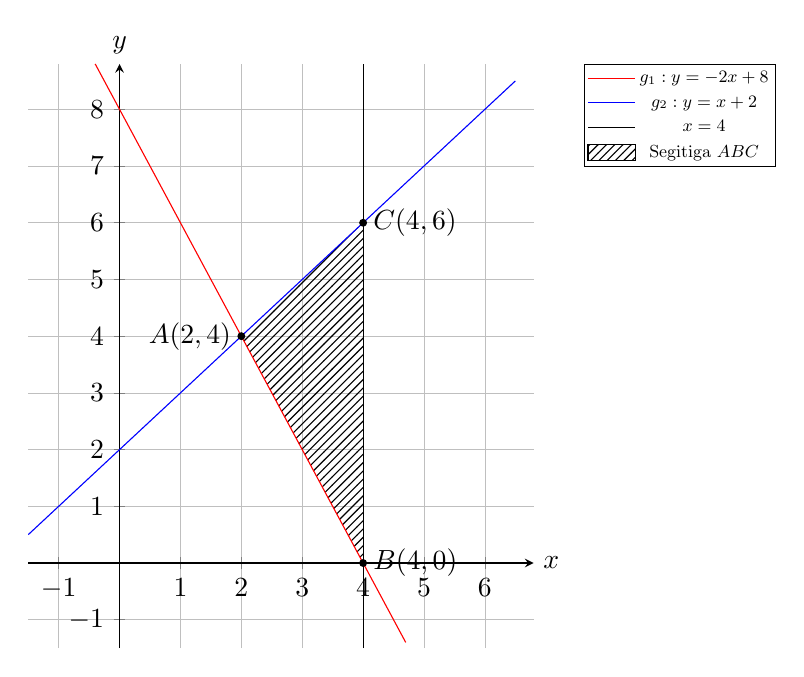
\begin{tikzpicture}
                   \begin{axis}[
        axis lines = middle,
        xlabel = $x$,
        ylabel = {$y$},
        grid=both,
        grid style={line width=.1pt, draw=gray!10},
        major grid style={line width=.2pt,draw=gray!50},
        x label style={anchor=west}, % label x ke kanan
        y label style={anchor=south}, % label y ke atas
        samples=200,
        legend style={
                at={(1.1,1)},
                anchor=north west,
                font=\small,         % mengecilkan ukuran font
                row sep=1pt,         % jarak antar baris legend
                inner sep=1pt,       % margin dalam kotak legend
                nodes={scale=0.7}    % skalakan isi legend
            },
        xtick={-1,0,...,6},
        ytick={-1,0,...,8},
        xmin=-1.5, xmax=6.8,
        ymin=-1.5, ymax=8.8,
        width=8cm,
        height=9cm
    ]
\addplot[opacity=0, domain=2:4, name path=A, forget plot] {-2*x+8};
\addplot[opacity=0, domain=2:4, name path=B, forget plot] {x+2};
\addplot[domain=-0.4:4.7, color=red] {-2*x+8};
\addlegendentry{$g_1: y=-2x+8$}
\addplot[domain=-1.5:6.5, color=blue] {x+2};
\addlegendentry{$g_2: y=x+2$}
\addplot[color=black] coordinates {(4,-1.5) (4,8.8)};
\addlegendentry{$x=4$}
\addplot[pattern=north east lines, area legend] fill between[of=A and B, soft clip={domain=2:4}];
\addlegendentry{Segitiga $ABC$}
\draw[fill=black, thick] (2,4) circle (1pt) node[left] {$A(2,4)$};
\draw[fill=black, thick] (4,0) circle (1pt) node[right] {$B(4,0)$};
\draw[fill=black, thick] (4,6) circle (1pt) node[right] {$C(4,6)$};
\end{axis}
                \end{tikzpicture}
            \end{center}
            Pandang garis $BC$ sebagai alas segitiga, sehingga panjang alasnya adalah $|6-0|=\colorlet{oldcolor}{.}
        \color{blue}
        \setlength{\fboxrule}{1pt} \boxed{\color{oldcolor}6}\color{oldcolor}$. Selanjutnya, pandang titik $A$ sebagai titik puncak segitiga, sehingga tinggi segitiga adalah jarak dari titik $A$ ke garis $BC$, yaitu jarak dari titik $(2,4)$ ke garis $x=4$, yang panjangnya adalah $|4-2|=\colorlet{oldcolor}{.}
        \color{blue}
        \setlength{\fboxrule}{1pt} \boxed{\color{oldcolor}2}\color{oldcolor}$. Dengan demikian, luas segitiga tersebut adalah
            \[
            L = \frac{1}{2} \times \text{alas} \times \text{tinggi} = \frac{1}{2} \times 6 \times 2 = \colorlet{oldcolor}{.}
        \color{red}
        \setlength{\fboxrule}{1pt} \boxed{\color{oldcolor}6}\color{oldcolor}.
            \]
        \end{enumerate}
    }
    \end{jawab}

    \item Diberikan $f(x)=\dfrac{1}{x^2-9}$ dan $g(x)=\sqrt{x+2}$.
    \begin{enumerate}
        \item Dapatkan domain $f(x)$ dan $g(x)$.
        \item Dapatkan $(f\circ g)(x)$ dan domain $(f\circ g)(x)$.
    \end{enumerate}
    \begin{jawab}[domain fungsi, fungsi komposisi, domain fungsi komposisi]{
        \begin{enumerate}
            \item Diperhatikan bahwa $f(x)$ merupakan fungsi rasional, sehingga domainnya adalah semua bilangan real kecuali nilai yang membuat penyebutnya sama dengan nol, yaitu $x^2-9=(x-3)(x+3)\neq 0$. Jadi
            \[
            \colorlet{oldcolor}{.}
        \color{red}
        \setlength{\fboxrule}{1pt} \boxed{\color{oldcolor}D(f)=\{x \in \mathbb{R} : x \neq -3,~x\neq 3\}=\mathbb{R}\setminus\{-3,3\}}\color{oldcolor}.
            \]
            Selanjutnya, diperhatikan bahwa $g(x)$ memuat akar kuadrat, sehingga domainnya adalah semua bilangan real yang membuat ekspresi di dalam akar kuadrat tak negatif, yaitu $x+2\geq 0$. Jadi
            \[
            \colorlet{oldcolor}{.}
        \color{red}
        \setlength{\fboxrule}{1pt} \boxed{\color{oldcolor}D(g)=\{x \in \mathbb{R} : x \geq -2\}=[-2,\infty)}\color{oldcolor}.
            \]
            \item Diperhatikan bahwa
            \begin{align*}
                (f\circ g)(x) = f(g(x)) = f(\sqrt{x+2}) = \frac{1}{(\sqrt{x+2})^2 - 9} = \frac{1}{x+2-9} = \colorlet{oldcolor}{.}
        \color{red}
        \setlength{\fboxrule}{1pt} \boxed{\color{oldcolor}\frac{1}{x-7}}\color{oldcolor}
            \end{align*}
            Domain dari fungsi komposisi $f\circ g$ adalah semua nilai $x$ pada domain $g$ sehingga nilai dari $g(x)$ berada pada domain $f$, yang dapat dirumuskan sebagai
            \begin{align*}
                \colorlet{oldcolor}{.}
        \color{blue}
        \setlength{\fboxrule}{1pt} \boxed{\color{oldcolor}D(f\circ g) = \{x \in D(g) : g(x) \in D(f)\} = \{x \in [-2, \infty) : \sqrt{x+2} \neq \pm 3\}}\color{oldcolor}.
            \end{align*}
            Karena $\sqrt{x+2}\geq 0$, maka $\sqrt{x+2}\neq -3$ selalu berlaku. Selanjutnya, $\sqrt{x+2} = 3$ jika dan hanya jika $x+2=9$, yang berarti $x = 7$. Didapatkan
            \begin{align*}
                \colorlet{oldcolor}{.}
        \color{red}
        \setlength{\fboxrule}{1pt} \boxed{\color{oldcolor}D(f\circ g) = [-2, \infty) \setminus \{7\} = [-2, 7) \cup (7, \infty)}\color{oldcolor}.
            \end{align*}
            \textit{Catatan:} meskipun bentuk akhir $\frac{1}{x-7}$ terdefinisi untuk $x<-2$, nilai-nilai tersebut tidak termasuk domain karena $g(x)$ tidak terdefinisi di sana.
        \end{enumerate}
    }
    \end{jawab}

    \item Diberikan fungsi sebagai berikut:
    \begin{align*}
        f(x)=\frac{2}{x-1};\quad \text{dan}\quad g(x)=\frac{x+2}{x}
    \end{align*}
    \begin{enumerate}
        \item Tentukan domain dan range dari masing-masing fungsi tersebut.
        \item Apakah kedua fungsi tersebut saling invers? Jelaskan alasannya.
    \end{enumerate}
    \begin{jawab}[domain dan range fungsi, fungsi rasional, fungsi invers, fungsi komposisi]{
        \begin{enumerate}
            \item Fungsi $f(x)=\frac{2}{x-1}$ terdefinisi untuk $x-1\neq 0$, sehingga $\colorlet{oldcolor}{.}
        \color{red}
        \setlength{\fboxrule}{1pt} \boxed{\color{oldcolor}D(f)=\mathbb{R}\setminus\{1\}}\color{oldcolor}$. Untuk menentukan range, misalkan $y=\frac{2}{x-1}$, maka
            \begin{align*}
                y(x-1) = 2 \iff x - 1 = \frac{2}{y} \iff x = 1+\frac{2}{y}.
            \end{align*}
            Nilai $x$ tersebut ada untuk setiap $y\neq 0$ (dan memang $\frac{2}{x-1}$ tidak pernah bernilai nol karena pembilangnya $2\neq 0$). Jadi $\colorlet{oldcolor}{.}
        \color{red}
        \setlength{\fboxrule}{1pt} \boxed{\color{oldcolor}R(f)=\mathbb{R}\setminus\{0\}}\color{oldcolor}$.\\
            Fungsi $g(x)=\frac{x+2}{x}$ terdefinisi untuk $x\neq 0$, sehingga $\colorlet{oldcolor}{.}
        \color{red}
        \setlength{\fboxrule}{1pt} \boxed{\color{oldcolor}D(g)=\mathbb{R}\setminus\{0\}}\color{oldcolor}$. Diperhatikan bahwa $g(x)=\frac{x+2}{x}=1+\frac{2}{x}$. Karena $\frac{2}{x}$ dapat bernilai sebarang bilangan real kecuali nol, maka $g(x)$ dapat bernilai sebarang bilangan real kecuali $1$. Jadi $\colorlet{oldcolor}{.}
        \color{red}
        \setlength{\fboxrule}{1pt} \boxed{\color{oldcolor}R(g)=\mathbb{R}\setminus\{1\}}\color{oldcolor}$.
            \item Dua fungsi $f$ dan $g$ saling invers jika
            \begin{align*}
                \colorlet{oldcolor}{.}
        \color{blue}
        \setlength{\fboxrule}{1pt} \boxed{\color{oldcolor}(f\circ g)(x)=x,~\forall x\in D(g)}\color{oldcolor} \quad\text{dan}\quad \colorlet{oldcolor}{.}
        \color{blue}
        \setlength{\fboxrule}{1pt} \boxed{\color{oldcolor}(g\circ f)(x)=x,~\forall x\in D(f)}\color{oldcolor}.
            \end{align*}
            Diperhatikan bahwa untuk $x\neq 0$,
            \begin{align*}
                (f\circ g)(x) = f\left(\frac{x+2}{x}\right) = \frac{2}{\frac{x+2}{x}-1} = \frac{2}{\frac{x+2-x}{x}} = \frac{2}{\frac{2}{x}} = x,
            \end{align*}
            dan untuk $x\neq 1$,
            \begin{align*}
                (g\circ f)(x) = g\left(\frac{2}{x-1}\right) = \frac{\frac{2}{x-1}+2}{\frac{2}{x-1}} = \frac{\frac{2+2(x-1)}{x-1}}{\frac{2}{x-1}} = \frac{2x}{2} = x.
            \end{align*}
            Selain itu, dari (a) terlihat bahwa $D(f)=R(g)=\mathbb{R}\setminus\{1\}$ dan $R(f)=D(g)=\mathbb{R}\setminus\{0\}$. Jadi $\colorlet{oldcolor}{.}
        \color{red}
        \setlength{\fboxrule}{1pt} \boxed{\color{oldcolor}f \text{ dan } g \text{ saling invers}}\color{oldcolor}$, yaitu $g=f^{-1}$ dan $f=g^{-1}$.
        \end{enumerate}
    }
    \end{jawab}

    \item Dapatkan nilai $k$ sedemikian sehingga fungsi:
    \begin{align*}
        f(x)=\begin{cases}
            kx^2-1, & x<2\\
            3x+k, & x\geq 2
        \end{cases}
    \end{align*}
    kontinu di $x=2$.
    \begin{jawab}[fungsi kontinu, limit sepihak, fungsi sepotong-sepotong]{~\\
        Ingat kembali syarat fungsi kontinu di suatu titik \(x = a\) adalah
        \begin{enumerate}
            \item \(f(a)\) terdefinisi
            \item \(\displaystyle \lim_{x \to a} f(x)\) ada, yaitu $\displaystyle \lim_{x \to a^-} f(x) = \lim_{x \to a^+} f(x)$
            \item \(\displaystyle\lim_{x \to a} f(x) = f(a)\)
        \end{enumerate}
        Diperhatikan bahwa untuk $x=2$ digunakan rumus $3x+k$, sehingga $\colorlet{oldcolor}{.}
        \color{blue}
        \setlength{\fboxrule}{1pt} \boxed{\color{oldcolor}f(2) = 6+k~\text{terdefinisi}}\color{oldcolor}$. Selanjutnya, limit kiri dan limit kanannya adalah
        \begin{align*}
            \lim_{x\to 2^-} f(x) = \lim_{x\to 2^-} (kx^2-1) = 4k-1 \quad\text{dan}\quad \lim_{x\to 2^+} f(x) = \lim_{x\to 2^+} (3x+k) = 6+k.
        \end{align*}
        Agar $f$ kontinu di $x=2$, haruslah $\colorlet{oldcolor}{.}
        \color{blue}
        \setlength{\fboxrule}{1pt} \boxed{\color{oldcolor}\lim_{x\to 2^-} f(x) = \lim_{x\to 2^+} f(x) = f(2)}\color{oldcolor}$, sehingga
        \begin{align*}
            4k-1 = 6+k \implies 3k = 7 \implies k = \frac{7}{3}.
        \end{align*}
        Jadi nilai $k$ yang membuat $f$ kontinu di $x=2$ adalah $\colorlet{oldcolor}{.}
        \color{red}
        \setlength{\fboxrule}{1pt} \boxed{\color{oldcolor}k=\frac{7}{3}}\color{oldcolor}$. Sebagai pengecekan, untuk $k=\frac{7}{3}$ diperoleh $4\left(\frac{7}{3}\right)-1=\frac{25}{3}$ dan $6+\frac{7}{3}=\frac{25}{3}$.
    }
    \end{jawab}

    \item Dapatkan $f'(x)$ untuk $x>\frac{1}{2}$, dimana $f(x)=\sqrt{\dfrac{(2x-1)^3}{x}}$.
    \begin{jawab}[turunan fungsi, aturan perkalian, aturan rantai]{~\\
        Karena $x>\frac{1}{2}$, maka $2x-1>0$ dan $x>0$, sehingga fungsi dapat ditulis dalam bentuk pangkat, yaitu
        \begin{align*}
            f(x) = \frac{(2x-1)^{3/2}}{x^{1/2}} = \colorlet{oldcolor}{.}
        \color{blue}
        \setlength{\fboxrule}{1pt} \boxed{\color{oldcolor}(2x-1)^{3/2}\cdot x^{-1/2}}\color{oldcolor}.
        \end{align*}
        Ingat kembali aturan perkalian, yaitu $\colorlet{oldcolor}{.}
        \color{blue}
        \setlength{\fboxrule}{1pt} \boxed{\color{oldcolor}(uv)'=u'v+uv'}\color{oldcolor}$. Misalkan $u=(2x-1)^{3/2}$ dan $v=x^{-1/2}$. Dengan aturan rantai diperoleh
        \begin{align*}
            \colorlet{oldcolor}{.}
        \color{blue}
        \setlength{\fboxrule}{1pt} \boxed{\color{oldcolor}u' = \frac{3}{2}(2x-1)^{1/2}\cdot 2 = 3(2x-1)^{1/2}}\color{oldcolor} \quad\text{dan}\quad \colorlet{oldcolor}{.}
        \color{blue}
        \setlength{\fboxrule}{1pt} \boxed{\color{oldcolor}v' = -\frac{1}{2}x^{-3/2}}\color{oldcolor}.
        \end{align*}
        Dengan demikian, diperoleh
        \begin{align*}
            f'(x) &= 3(2x-1)^{1/2}x^{-1/2} + (2x-1)^{3/2}\left(-\frac{1}{2}x^{-3/2}\right)\\
            &= (2x-1)^{1/2}x^{-3/2}\left[3x - \frac{1}{2}(2x-1)\right]\\
            &= (2x-1)^{1/2}x^{-3/2}\cdot\frac{6x-2x+1}{2}\\
            &= \colorlet{oldcolor}{.}
        \color{red}
        \setlength{\fboxrule}{1pt} \boxed{\color{oldcolor}\frac{(4x+1)\sqrt{2x-1}}{2x\sqrt{x}}}\color{oldcolor}.
        \end{align*}
    }
    \end{jawab}
\end{enumerate}

\newpage

%%%%%%%%%%%%%%%%%%%%%%%%%%%%%%%%%%%%%%%%%%%%%%%%%%%%%%%%%%%%%%%%%%%%%%%%%%%%%%
% Kal-iup-1
\kopsoaliup{Kal-iup-1}{61, 68}{Chemical, Environmental, Electrical Engineering}{Monday, Wednesday; 07.00-09.30}{1}
\begin{enumerate}
    \item Solve the following inequality.
    \begin{align*}
        \frac{x^2-2x-8}{x^2-4x+3}\geq 0.
    \end{align*}
    \begin{jawab}[pertidaksamaan rasional, faktorisasi, garis bilangan, notasi interval]{~\\
    Karena ruas kanan pertidaksamaan sudah bernilai nol, maka kita bisa langsung memfaktorkan pembilang dan penyebut di ruas kiri. Diperoleh
    \begin{align*}
        \frac{x^2-2x-8}{x^2-4x+3} = \frac{(x-4)(x+2)}{(x-1)(x-3)} \geq 0.
    \end{align*}
    Selanjutnya, kita tentukan pembuat nol dari faktor-faktor tersebut, yaitu
    \begin{align*}
        x-4 = 0 \quad &\vee\quad x+2 = 0 \quad \vee\quad x-1 = 0 \quad \vee\quad x-3 = 0\\
        \colorlet{oldcolor}{.}
        \color{blue}
        \setlength{\fboxrule}{1pt} \boxed{\color{oldcolor}x=4}\color{oldcolor} \quad &\vee\quad \colorlet{oldcolor}{.}
        \color{blue}
        \setlength{\fboxrule}{1pt} \boxed{\color{oldcolor}x=-2}\color{oldcolor} \quad \vee\quad \colorlet{oldcolor}{.}
        \color{blue}
        \setlength{\fboxrule}{1pt} \boxed{\color{oldcolor}x=1}\color{oldcolor} \quad \vee\quad \colorlet{oldcolor}{.}
        \color{blue}
        \setlength{\fboxrule}{1pt} \boxed{\color{oldcolor}x=3}\color{oldcolor}
    \end{align*}
    Selanjutnya, kita buat garis bilangan dan lakukan uji titik pada ekspresi \(\frac{(x-4)(x+2)}{(x-1)(x-3)}\) sebagai berikut
    \begin{itemize}
        \item Untuk \(x < -2\), misalkan \(x = -3\):
        \[
        \frac{(-3-4)(-3+2)}{(-3-1)(-3-3)} = \frac{(-7)(-1)}{(-4)(-6)} = \frac{7}{24} > 0
        \]
        \item Untuk \(-2 < x < 1\), misalkan \(x = 0\):
        \[
        \frac{(0-4)(0+2)}{(0-1)(0-3)} = \frac{(-4)(2)}{(-1)(-3)} = \frac{-8}{3} < 0
        \]
        \item Untuk \(1 < x < 3\), misalkan \(x = 2\):
        \[
        \frac{(2-4)(2+2)}{(2-1)(2-3)} = \frac{(-2)(4)}{(1)(-1)} = 8 > 0
        \]
        \item Untuk \(3 < x < 4\), misalkan \(x = 3.5\):
        \[
        \frac{(3.5-4)(3.5+2)}{(3.5-1)(3.5-3)} = \frac{(-0.5)(5.5)}{(2.5)(0.5)} = \frac{-2.75}{1.25} < 0
        \]
        \item Untuk \(x > 4\), misalkan \(x = 5\):
        \[
        \frac{(5-4)(5+2)}{(5-1)(5-3)} = \frac{(1)(7)}{(4)(2)} = \frac{7}{8} > 0
        \]
    \end{itemize}
    \begin{center}
        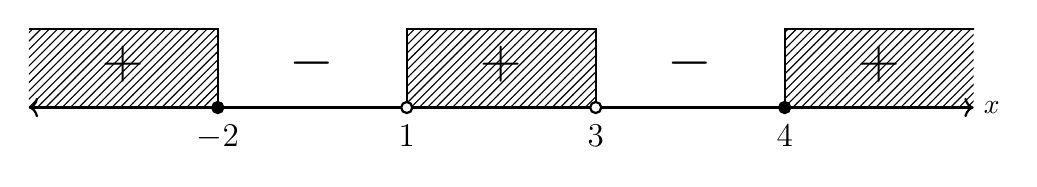
\begin{tikzpicture}
    \draw[thick,<->] (-6,0) -- (6,0) node[right] {$x$};
    \fill[pattern=north east lines] (-6,0) rectangle (-3.6,1);
    \fill[pattern=north east lines] (-1.2,0) rectangle (1.2,1);
    \fill[pattern=north east lines] (3.6,0) rectangle (6,1);
    \draw[thick] (-6,1) -- (-3.6,1) -- (-3.6,0);
    \draw[thick] (-1.2,0) -- (-1.2,1) -- (1.2,1) -- (1.2,0);
    \draw[thick] (3.6,0) -- (3.6,1) -- (6,1);
    \draw (-3.6,-0.1) node[below] {\large{$-2$}};
    \draw (-1.2,-0.1) node[below] {\large{$1$}};
    \draw (1.2,-0.1) node[below] {\large{$3$}};
    \draw (3.6,-0.1) node[below] {\large{$4$}};
    \draw (-4.8,0.2) node[above] {\huge{$+$}};
    \draw (-2.4,0.2) node[above] {\huge{$-$}};
    \draw (0,0.2) node[above] {\huge{$+$}};
    \draw (2.4,0.2) node[above] {\huge{$-$}};
    \draw (4.8,0.2) node[above] {\huge{$+$}};
    \draw[fill=black, thick] (-3.6,0) circle (2pt);
    \draw[fill=white, thick] (-1.2,0) circle (2pt);
    \draw[fill=white, thick] (1.2,0) circle (2pt);
    \draw[fill=black, thick] (3.6,0) circle (2pt);
        \end{tikzpicture}
    \end{center}
    Karena yang diminta adalah nilai yang lebih dari atau sama dengan nol, diambil interval yang bertanda positif beserta pembuat nol dari pembilang ($x=-2$ dan $x=4$). Pembuat nol dari penyebut ($x=1$ dan $x=3$) tidak diikutkan karena membuat ekspresi tidak terdefinisi. Jadi solusi dari pertidaksamaan tersebut adalah \(x \leq -2\) atau \(1 < x < 3\) atau \(x \geq 4\). Dalam notasi interval, solusi tersebut dapat ditulis sebagai $\colorlet{oldcolor}{.}
        \color{red}
        \setlength{\fboxrule}{1pt} \boxed{\color{oldcolor}(-\infty, -2] \cup (1, 3) \cup [4, \infty)}\color{oldcolor}$.
    }
    \end{jawab}

    \item Given a function $f(x)=3-\sqrt{x}$ and $g(x)=\dfrac{1}{x+1}$. Determine:
    \begin{enumerate}
        \item[a)] The domain of function $f$ and $g$;
        \item[b)] Function $(f\circ g)(x)$ and its domain.
    \end{enumerate}
    \begin{jawab}[domain fungsi, fungsi komposisi, domain fungsi komposisi]{
        \begin{enumerate}
            \item Diperhatikan bahwa $f(x)$ memuat akar kuadrat, sehingga domainnya adalah semua bilangan real yang membuat ekspresi di dalam akar kuadrat tak negatif. Jadi
            \begin{align*}
                \colorlet{oldcolor}{.}
        \color{red}
        \setlength{\fboxrule}{1pt} \boxed{\color{oldcolor}D(f)=\{x \in \mathbb{R} : x \geq 0\}}\color{oldcolor}.
            \end{align*}
            Selanjutnya, diperhatikan bahwa $g(x)$ merupakan fungsi rasional, sehingga domainnya adalah semua bilangan real kecuali nilai yang membuat penyebutnya sama dengan nol, yaitu $x+1\neq 0$. Jadi
            \begin{align*}
                \colorlet{oldcolor}{.}
        \color{red}
        \setlength{\fboxrule}{1pt} \boxed{\color{oldcolor}D(g)=\{x \in \mathbb{R} : x \neq -1\}}\color{oldcolor}.
            \end{align*}
            \item Diperhatikan bahwa
            \begin{align*}
                (f\circ g)(x) = f(g(x)) = f\left(\frac{1}{x+1}\right) = 3 - \sqrt{\frac{1}{x+1}} = \colorlet{oldcolor}{.}
        \color{red}
        \setlength{\fboxrule}{1pt} \boxed{\color{oldcolor}3 - \frac{1}{\sqrt{x+1}}}\color{oldcolor}
            \end{align*}
            Domain dari fungsi komposisi $f\circ g$ adalah semua nilai $x$ pada domain $g$ sehingga nilai dari $g(x)$ berada pada domain $f$, yang dapat dirumuskan sebagai
            \begin{align*}
                \colorlet{oldcolor}{.}
        \color{blue}
        \setlength{\fboxrule}{1pt} \boxed{\color{oldcolor}D(f\circ g) = \{x \in D(g) : g(x) \in D(f)\} = \left\{x \neq -1 : \frac{1}{x+1} \geq 0\right\}}\color{oldcolor}.
            \end{align*}
            Karena pembilangnya bernilai $1>0$, maka $\frac{1}{x+1} \geq 0$ jika dan hanya jika $x+1 > 0$, yang berarti $x > -1$. Didapatkan
            \begin{align*}
                \colorlet{oldcolor}{.}
        \color{red}
        \setlength{\fboxrule}{1pt} \boxed{\color{oldcolor}D(f\circ g) = (-1, \infty)}\color{oldcolor}.
            \end{align*}
        \end{enumerate}
    }
    \end{jawab}

    \item Write the derivative formula of $\dfrac{f}{g}$, that is $\dfrac{d}{dx}\left(\dfrac{f(x)}{g(x)}\right)$.\\
    Then, find the derivative of $\dfrac{f}{g}$ given that $f(x)=x^2+4x-5$ and $g(x)=x+2$ for $x\neq -2$.
    \begin{jawab}[turunan, aturan pembagian]{~\\
        Ingat kembali aturan turunan untuk pembagian fungsi, yaitu
        \[
        \colorlet{oldcolor}{.}
        \color{red}
        \setlength{\fboxrule}{1pt} \boxed{\color{oldcolor}\frac{d}{dx}\left(\frac{f(x)}{g(x)}\right) = \frac{f'(x)g(x) - f(x)g'(x)}{(g(x))^2}}\color{oldcolor}.
        \]
        Selanjutnya, kita hitung turunan dari \(f(x)\) dan \(g(x)\):
        \begin{align*}
            \colorlet{oldcolor}{.}
        \color{blue}
        \setlength{\fboxrule}{1pt} \boxed{\color{oldcolor}f'(x) = \frac{d}{dx}(x^2 + 4x - 5) = 2x + 4}\color{oldcolor}\\
            \colorlet{oldcolor}{.}
        \color{blue}
        \setlength{\fboxrule}{1pt} \boxed{\color{oldcolor}g'(x) = \frac{d}{dx}(x + 2) = 1}\color{oldcolor}
        \end{align*}
        Dengan demikian, turunan dari \(\frac{f}{g}\) adalah
        \begin{align*}
            \frac{d}{dx}\left(\frac{f(x)}{g(x)}\right) &= \frac{(2x + 4)(x + 2) - (x^2 + 4x - 5)(1)}{(x + 2)^2}\\
            &= \frac{(2x^2 + 8x + 8) - (x^2 + 4x - 5)}{(x + 2)^2}\\
            &= \colorlet{oldcolor}{.}
        \color{red}
        \setlength{\fboxrule}{1pt} \boxed{\color{oldcolor}\frac{x^2 + 4x + 13}{(x + 2)^2}}\color{oldcolor}.
        \end{align*}
    }
    \end{jawab}

    \item Given $f(x)=\begin{cases}
        \dfrac{x^3+27}{x+3}, & x\neq -3\\
        3k, & x=-3
    \end{cases}$.
    \begin{enumerate}
        \item[a.] Determine $k$ such that $f(x)$ is continuous at $x=-3$.
        \item[b.] Based on the result of a), rewrite $f(x)$ as a polynomial.
    \end{enumerate}
    \begin{jawab}[fungsi kontinu, limit, polinomial]{
        \begin{enumerate}
            \item Ingat kembali syarat fungsi kontinu di suatu titik \(x = a\) adalah
            \begin{enumerate}
                \item \(f(a)\) terdefinisi
                \item \(\displaystyle \lim_{x \to a} f(x)\) ada, yaitu $\displaystyle \lim_{x \to a^-} f(x) = \lim_{x \to a^+} f(x)$
                \item \(\displaystyle\lim_{x \to a} f(x) = f(a)\)
            \end{enumerate}
            Diperhatikan bahwa untuk \(x = -3\), $\colorlet{oldcolor}{.}
        \color{blue}
        \setlength{\fboxrule}{1pt} \boxed{\color{oldcolor}f(-3) = 3k~\text{terdefinisi}}\color{oldcolor}$. Karena limit di $x=-3$ artinya nilai fungsi di sekitar $x=-3$ tetapi $x\neq -3$, dan dengan rumus $a^3+b^3=(a+b)(a^2-ab+b^2)$, didapatkan limitnya adalah
            \begin{align*}
            \lim_{x \to -3} f(x) = \lim_{x \to -3} \frac{x^3 + 27}{x + 3} = \lim_{x \to -3} \frac{(x+3)(x^2 - 3x + 9)}{x+3} = \lim_{x \to -3} (x^2 - 3x + 9) = 9+9+9 = \colorlet{oldcolor}{.}
        \color{blue}
        \setlength{\fboxrule}{1pt} \boxed{\color{oldcolor}27}\color{oldcolor}.
            \end{align*}
            Selanjutnya, untuk syarat ketiga, haruslah $\displaystyle\lim_{x \to -3} f(x) = f(-3)$, sehingga diperoleh $27 = 3k$, dan didapatkan $\colorlet{oldcolor}{.}
        \color{red}
        \setlength{\fboxrule}{1pt} \boxed{\color{oldcolor}k=9}\color{oldcolor}$.
        \item Diperhatikan bahwa untuk $x\neq -3$, berlaku
        \begin{align*}
            f(x) = \frac{x^3 + 27}{x + 3} = \frac{(x+3)(x^2 - 3x + 9)}{x+3} = x^2 - 3x + 9.
        \end{align*}
        Berdasarkan hasil dari (a), diperoleh bahwa \(f(x)\) kontinu di \(x=-3\) jika \(k=9\), yaitu $f(-3)=27$, yang sama dengan nilai polinomial di atas saat $x=-3$. Dengan demikian, fungsi \(f(x)\) dapat dinyatakan sebagai polinomial
        \begin{align*}
            \colorlet{oldcolor}{.}
        \color{red}
        \setlength{\fboxrule}{1pt} \boxed{\color{oldcolor}f(x) = x^2 - 3x + 9}\color{oldcolor}.
        \end{align*}
        \end{enumerate}
    }
    \end{jawab}

    \item Sketch the base curve $x=y^2$. Based on that base curve, use translation to sketch the curve $x=y^2-2y-3$. (Explain the process).
    \begin{jawab}[parabola, melengkapkan kuadrat, translasi grafik]{~\\
        Kurva dasar $x=y^2$ merupakan parabola yang terbuka ke kanan dengan titik puncak $(0,0)$. Selanjutnya, bentuk $x = y^2 - 2y - 3$ diubah dengan cara melengkapkan kuadrat, yaitu
        \begin{align*}
            x &= y^2 - 2y - 3\\
            &= (y^2 - 2y + 1) - 1 - 3\\
            &= \colorlet{oldcolor}{.}
        \color{blue}
        \setlength{\fboxrule}{1pt} \boxed{\color{oldcolor}(y-1)^2 - 4}\color{oldcolor}.
        \end{align*}
        Ingat kembali bahwa mengganti $y$ dengan $y-1$ berarti menggeser grafik sejauh $1$ satuan ke atas, dan menambahkan konstanta $-4$ pada $x$ berarti menggeser grafik sejauh $4$ satuan ke kiri. Dengan demikian, proses translasinya adalah sebagai berikut.
        \begin{enumerate}
            \item[(i)] Gambar kurva dasar $x=y^2$ dengan titik puncak $(0,0)$.
            \item[(ii)] Geser kurva $x=y^2$ sejauh $1$ satuan ke atas, sehingga diperoleh kurva $x=(y-1)^2$ dengan titik puncak $(0,1)$.
            \item[(iii)] Geser kurva $x=(y-1)^2$ sejauh $4$ satuan ke kiri, sehingga diperoleh kurva $x=(y-1)^2-4$ dengan titik puncak $\colorlet{oldcolor}{.}
        \color{blue}
        \setlength{\fboxrule}{1pt} \boxed{\color{oldcolor}(-4,1)}\color{oldcolor}$.
        \end{enumerate}
        Sebagai bantuan, titik potong kurva dengan sumbu-$x$ ($y=0$) adalah $x=-3$, yaitu titik $(-3,0)$, sedangkan titik potong dengan sumbu-$y$ ($x=0$) adalah $(y-1)^2=4$, yaitu $y=-1$ dan $y=3$. Sketsa grafiknya adalah sebagai berikut.
        \begin{center}
            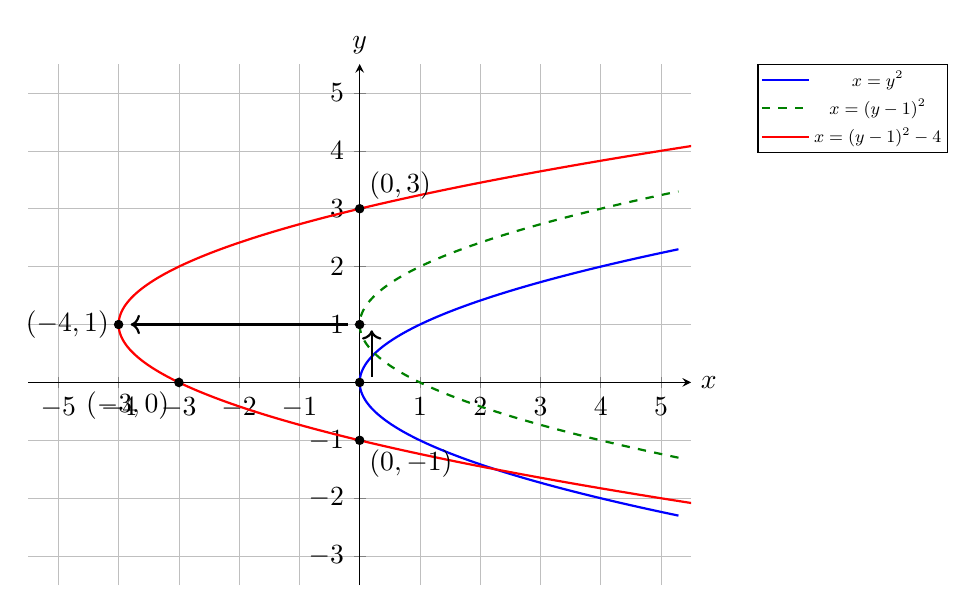
\begin{tikzpicture}
                \begin{axis}[
        axis lines = middle,
        xlabel = $x$,
        ylabel = {$y$},
        grid=both,
        grid style={line width=.1pt, draw=gray!10},
        major grid style={line width=.2pt,draw=gray!50},
        x label style={anchor=west}, % label x ke kanan
        y label style={anchor=south}, % label y ke atas
        samples=200,
        legend style={
                at={(1.1,1)},
                anchor=north west,
                font=\small,         % mengecilkan ukuran font
                row sep=1pt,         % jarak antar baris legend
                inner sep=1pt,       % margin dalam kotak legend
                nodes={scale=0.7}    % skalakan isi legend
            },
        xtick={-5,-4,...,5},
        ytick={-3,-2,...,5},
        xmin=-5.5, xmax=5.5,
        ymin=-3.5, ymax=5.5,
        width=10cm,
        height=8.2cm
    ]
\addplot[domain=-2.3:2.3, color=blue, thick] ({(x)*(x)},{x});
\addlegendentry{$x=y^2$}
\addplot[domain=-1.3:3.3, color=green!50!black, thick, dashed] ({(x-1)*(x-1)},{x});
\addlegendentry{$x=(y-1)^2$}
\addplot[domain=-2.2:4.2, color=red, thick] ({(x-1)*(x-1)-4},{x});
\addlegendentry{$x=(y-1)^2-4$}
\draw[fill=black] (0,0) circle (1.5pt);
\draw[fill=black] (0,1) circle (1.5pt);
\draw[fill=black] (-4,1) circle (1.5pt) node[left] {$(-4,1)$};
\draw[fill=black] (-3,0) circle (1.5pt) node[below left] {$(-3,0)$};
\draw[fill=black] (0,3) circle (1.5pt) node[above right] {$(0,3)$};
\draw[fill=black] (0,-1) circle (1.5pt) node[below right] {$(0,-1)$};
\draw[->, thick] (0.2,0.1) -- (0.2,0.9);
\draw[->, thick] (-0.2,1) -- (-3.8,1);
\end{axis}
            \end{tikzpicture}
        \end{center}
        Jadi kurva $x = y^2 - 2y - 3$ adalah
        \[\colorlet{oldcolor}{.}
        \color{red}
        \setlength{\fboxrule}{1pt} \boxed{\color{oldcolor}\text{parabola } x=y^2 \text{ yang digeser 1 satuan ke atas dan 4 satuan ke kiri}}\color{oldcolor}.\]
    }
    \end{jawab}
\end{enumerate}

\newpage

%%%%%%%%%%%%%%%%%%%%%%%%%%%%%%%%%%%%%%%%%%%%%%%%%%%%%%%%%%%%%%%%%%%%%%%%%%%%%%
% Kal-iup-4
\kopsoaliup{Kal-iup-4}{65, 66, 67}{Statistics, Marine Engineering (JD), Informatics}{Monday, Wednesday; 07.00-09.30}{1}
\begin{enumerate}
    \item Solve the following inequality.
    \begin{align*}
        \frac{x^2+2x-15}{x^2-x-2}\geq 0.
    \end{align*}
    \begin{jawab}[pertidaksamaan rasional, faktorisasi, garis bilangan, notasi interval]{~\\
    Karena ruas kanan pertidaksamaan sudah bernilai nol, maka kita bisa langsung memfaktorkan pembilang dan penyebut di ruas kiri. Diperoleh
    \begin{align*}
        \frac{x^2+2x-15}{x^2-x-2} = \frac{(x+5)(x-3)}{(x-2)(x+1)} \geq 0.
    \end{align*}
    Selanjutnya, kita tentukan pembuat nol dari faktor-faktor tersebut, yaitu
    \begin{align*}
        x+5 = 0 \quad &\vee\quad x-3 = 0 \quad \vee\quad x-2 = 0 \quad \vee\quad x+1 = 0\\
        \colorlet{oldcolor}{.}
        \color{blue}
        \setlength{\fboxrule}{1pt} \boxed{\color{oldcolor}x=-5}\color{oldcolor} \quad &\vee\quad \colorlet{oldcolor}{.}
        \color{blue}
        \setlength{\fboxrule}{1pt} \boxed{\color{oldcolor}x=3}\color{oldcolor} \quad \vee\quad \colorlet{oldcolor}{.}
        \color{blue}
        \setlength{\fboxrule}{1pt} \boxed{\color{oldcolor}x=2}\color{oldcolor} \quad \vee\quad \colorlet{oldcolor}{.}
        \color{blue}
        \setlength{\fboxrule}{1pt} \boxed{\color{oldcolor}x=-1}\color{oldcolor}
    \end{align*}
    Selanjutnya, kita buat garis bilangan dan lakukan uji titik pada ekspresi \(\frac{(x+5)(x-3)}{(x-2)(x+1)}\) sebagai berikut
    \begin{itemize}
        \item Untuk \(x < -5\), misalkan \(x = -6\):
        \[
        \frac{(-6+5)(-6-3)}{(-6-2)(-6+1)} = \frac{(-1)(-9)}{(-8)(-5)} = \frac{9}{40} > 0
        \]
        \item Untuk \(-5 < x < -1\), misalkan \(x = -2\):
        \[
        \frac{(-2+5)(-2-3)}{(-2-2)(-2+1)} = \frac{(3)(-5)}{(-4)(-1)} = \frac{-15}{4} < 0
        \]
        \item Untuk \(-1 < x < 2\), misalkan \(x = 0\):
        \[
        \frac{(0+5)(0-3)}{(0-2)(0+1)} = \frac{(5)(-3)}{(-2)(1)} = \frac{15}{2} > 0
        \]
        \item Untuk \(2 < x < 3\), misalkan \(x = 2.5\):
        \[
        \frac{(2.5+5)(2.5-3)}{(2.5-2)(2.5+1)} = \frac{(7.5)(-0.5)}{(0.5)(3.5)} = \frac{-3.75}{1.75} < 0
        \]
        \item Untuk \(x > 3\), misalkan \(x = 4\):
        \[
        \frac{(4+5)(4-3)}{(4-2)(4+1)} = \frac{(9)(1)}{(2)(5)} = \frac{9}{10} > 0
        \]
    \end{itemize}
    \begin{center}
        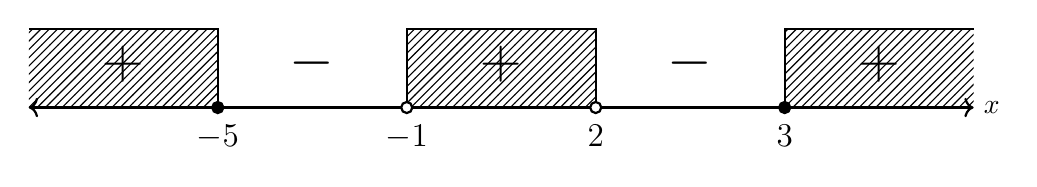
\begin{tikzpicture}
    \draw[thick,<->] (-6,0) -- (6,0) node[right] {$x$};
    \fill[pattern=north east lines] (-6,0) rectangle (-3.6,1);
    \fill[pattern=north east lines] (-1.2,0) rectangle (1.2,1);
    \fill[pattern=north east lines] (3.6,0) rectangle (6,1);
    \draw[thick] (-6,1) -- (-3.6,1) -- (-3.6,0);
    \draw[thick] (-1.2,0) -- (-1.2,1) -- (1.2,1) -- (1.2,0);
    \draw[thick] (3.6,0) -- (3.6,1) -- (6,1);
    \draw (-3.6,-0.1) node[below] {\large{$-5$}};
    \draw (-1.2,-0.1) node[below] {\large{$-1$}};
    \draw (1.2,-0.1) node[below] {\large{$2$}};
    \draw (3.6,-0.1) node[below] {\large{$3$}};
    \draw (-4.8,0.2) node[above] {\huge{$+$}};
    \draw (-2.4,0.2) node[above] {\huge{$-$}};
    \draw (0,0.2) node[above] {\huge{$+$}};
    \draw (2.4,0.2) node[above] {\huge{$-$}};
    \draw (4.8,0.2) node[above] {\huge{$+$}};
    \draw[fill=black, thick] (-3.6,0) circle (2pt);
    \draw[fill=white, thick] (-1.2,0) circle (2pt);
    \draw[fill=white, thick] (1.2,0) circle (2pt);
    \draw[fill=black, thick] (3.6,0) circle (2pt);
        \end{tikzpicture}
    \end{center}
    Karena yang diminta adalah nilai yang lebih dari atau sama dengan nol, diambil interval yang bertanda positif beserta pembuat nol dari pembilang ($x=-5$ dan $x=3$). Pembuat nol dari penyebut ($x=-1$ dan $x=2$) tidak diikutkan karena membuat ekspresi tidak terdefinisi. Jadi solusi dari pertidaksamaan tersebut adalah \(x \leq -5\) atau \(-1 < x < 2\) atau \(x \geq 3\). Dalam notasi interval, solusi tersebut dapat ditulis sebagai $\colorlet{oldcolor}{.}
        \color{red}
        \setlength{\fboxrule}{1pt} \boxed{\color{oldcolor}(-\infty, -5] \cup (-1, 2) \cup [3, \infty)}\color{oldcolor}$.
    }
    \end{jawab}

    \item Given a function $f(x)=1-\sqrt{x}$ and $g(x)=\dfrac{4}{x-2}$. Determine:
    \begin{enumerate}
        \item[a)] The domain of function $f$ and $g$;
        \item[b)] Function $(f\circ g)(x)$ and its domain.
    \end{enumerate}
    \begin{jawab}[domain fungsi, fungsi komposisi, domain fungsi komposisi]{
        \begin{enumerate}
            \item Diperhatikan bahwa $f(x)$ memuat akar kuadrat, sehingga domainnya adalah semua bilangan real yang membuat ekspresi di dalam akar kuadrat tak negatif. Jadi
            \begin{align*}
                \colorlet{oldcolor}{.}
        \color{red}
        \setlength{\fboxrule}{1pt} \boxed{\color{oldcolor}D(f)=\{x \in \mathbb{R} : x \geq 0\}}\color{oldcolor}.
            \end{align*}
            Selanjutnya, diperhatikan bahwa $g(x)$ merupakan fungsi rasional, sehingga domainnya adalah semua bilangan real kecuali nilai yang membuat penyebutnya sama dengan nol, yaitu $x-2\neq 0$. Jadi
            \begin{align*}
                \colorlet{oldcolor}{.}
        \color{red}
        \setlength{\fboxrule}{1pt} \boxed{\color{oldcolor}D(g)=\{x \in \mathbb{R} : x \neq 2\}}\color{oldcolor}.
            \end{align*}
            \item Diperhatikan bahwa
            \begin{align*}
                (f\circ g)(x) = f(g(x)) = f\left(\frac{4}{x-2}\right) = 1 - \sqrt{\frac{4}{x-2}} = \colorlet{oldcolor}{.}
        \color{red}
        \setlength{\fboxrule}{1pt} \boxed{\color{oldcolor}1 - \frac{2}{\sqrt{x-2}}}\color{oldcolor}
            \end{align*}
            Domain dari fungsi komposisi $f\circ g$ adalah semua nilai $x$ pada domain $g$ sehingga nilai dari $g(x)$ berada pada domain $f$, yang dapat dirumuskan sebagai
            \begin{align*}
                \colorlet{oldcolor}{.}
        \color{blue}
        \setlength{\fboxrule}{1pt} \boxed{\color{oldcolor}D(f\circ g) = \{x \in D(g) : g(x) \in D(f)\} = \left\{x \neq 2 : \frac{4}{x-2} \geq 0\right\}}\color{oldcolor}.
            \end{align*}
            Karena pembilangnya bernilai $4>0$, maka $\frac{4}{x-2} \geq 0$ jika dan hanya jika $x-2 > 0$, yang berarti $x > 2$. Didapatkan
            \begin{align*}
                \colorlet{oldcolor}{.}
        \color{red}
        \setlength{\fboxrule}{1pt} \boxed{\color{oldcolor}D(f\circ g) = (2, \infty)}\color{oldcolor}.
            \end{align*}
        \end{enumerate}
    }
    \end{jawab}

    \item Write the derivative formula of $\dfrac{f}{g}$, that is $\dfrac{d}{dx}\left(\dfrac{f(x)}{g(x)}\right)$.\\
    Then, find the derivative of $\dfrac{f}{g}$ given that $f(x)=3x^2-5x-2$ and $g(x)=x-2$ for $x\neq 2$.
    \begin{jawab}[turunan, aturan pembagian]{~\\
        Ingat kembali aturan turunan untuk pembagian fungsi, yaitu
        \[
        \colorlet{oldcolor}{.}
        \color{red}
        \setlength{\fboxrule}{1pt} \boxed{\color{oldcolor}\frac{d}{dx}\left(\frac{f(x)}{g(x)}\right) = \frac{f'(x)g(x) - f(x)g'(x)}{(g(x))^2}}\color{oldcolor}.
        \]
        Selanjutnya, kita hitung turunan dari \(f(x)\) dan \(g(x)\):
        \begin{align*}
            \colorlet{oldcolor}{.}
        \color{blue}
        \setlength{\fboxrule}{1pt} \boxed{\color{oldcolor}f'(x) = \frac{d}{dx}(3x^2 - 5x - 2) = 6x - 5}\color{oldcolor}\\
            \colorlet{oldcolor}{.}
        \color{blue}
        \setlength{\fboxrule}{1pt} \boxed{\color{oldcolor}g'(x) = \frac{d}{dx}(x - 2) = 1}\color{oldcolor}
        \end{align*}
        Dengan demikian, turunan dari \(\frac{f}{g}\) adalah
        \begin{align*}
            \frac{d}{dx}\left(\frac{f(x)}{g(x)}\right) &= \frac{(6x - 5)(x - 2) - (3x^2 - 5x - 2)(1)}{(x - 2)^2}\\
            &= \frac{(6x^2 - 17x + 10) - (3x^2 - 5x - 2)}{(x - 2)^2}\\
            &= \frac{3x^2 - 12x + 12}{(x - 2)^2}\\
            &= \frac{3(x-2)^2}{(x - 2)^2}\\
            &= \colorlet{oldcolor}{.}
        \color{red}
        \setlength{\fboxrule}{1pt} \boxed{\color{oldcolor}3}\color{oldcolor}, \quad x\neq 2.
        \end{align*}
        Hasil ini masuk akal, karena $f(x)=3x^2-5x-2=(3x+1)(x-2)$, sehingga untuk $x\neq 2$ berlaku $\frac{f(x)}{g(x)}=3x+1$ yang turunannya adalah $3$.
    }
    \end{jawab}

    \item Given $f(x)=\begin{cases}
        \dfrac{x^3-1}{2x-2}, & x\neq 1\\
        3k, & x=1
    \end{cases}$.
    \begin{enumerate}
        \item[a.] Determine $k$ such that $f(x)$ is continuous at $x=1$.
        \item[b.] Based on the result of a), rewrite $f(x)$ as a polynomial.
    \end{enumerate}
    \begin{jawab}[fungsi kontinu, limit, polinomial]{
        \begin{enumerate}
            \item Ingat kembali syarat fungsi kontinu di suatu titik \(x = a\) adalah
            \begin{enumerate}
                \item \(f(a)\) terdefinisi
                \item \(\displaystyle \lim_{x \to a} f(x)\) ada, yaitu $\displaystyle \lim_{x \to a^-} f(x) = \lim_{x \to a^+} f(x)$
                \item \(\displaystyle\lim_{x \to a} f(x) = f(a)\)
            \end{enumerate}
            Diperhatikan bahwa untuk \(x = 1\), $\colorlet{oldcolor}{.}
        \color{blue}
        \setlength{\fboxrule}{1pt} \boxed{\color{oldcolor}f(1) = 3k~\text{terdefinisi}}\color{oldcolor}$. Karena limit di $x=1$ artinya nilai fungsi di sekitar $x=1$ tetapi $x\neq 1$, didapatkan limitnya adalah
            \begin{align*}
            \lim_{x \to 1} f(x) = \lim_{x \to 1} \frac{x^3 - 1}{2x - 2} = \lim_{x \to 1} \frac{(x-1)(x^2 + x + 1)}{2(x-1)} = \lim_{x \to 1} \frac{x^2 + x + 1}{2} = \colorlet{oldcolor}{.}
        \color{blue}
        \setlength{\fboxrule}{1pt} \boxed{\color{oldcolor}\frac{3}{2}}\color{oldcolor}.
            \end{align*}
            Selanjutnya, untuk syarat ketiga, haruslah $\displaystyle\lim_{x \to 1} f(x) = f(1)$, sehingga diperoleh $\frac{3}{2} = 3k$, dan didapatkan $\colorlet{oldcolor}{.}
        \color{red}
        \setlength{\fboxrule}{1pt} \boxed{\color{oldcolor}k=\frac{1}{2}}\color{oldcolor}$.
        \item Diperhatikan bahwa untuk $x\neq 1$, berlaku
        \begin{align*}
            f(x) = \frac{x^3 - 1}{2x - 2} = \frac{(x-1)(x^2 + x + 1)}{2(x-1)} = \frac{x^2 + x + 1}{2} = \frac{1}{2}x^2 + \frac{1}{2}x + \frac{1}{2}.
        \end{align*}
        Berdasarkan hasil dari (a), diperoleh bahwa \(f(x)\) kontinu di \(x=1\) jika \(k=\frac{1}{2}\), yaitu $f(1)=\frac{3}{2}$, yang sama dengan nilai polinomial di atas saat $x=1$. Dengan demikian, fungsi \(f(x)\) dapat dinyatakan sebagai polinomial
        \begin{align*}
            \colorlet{oldcolor}{.}
        \color{red}
        \setlength{\fboxrule}{1pt} \boxed{\color{oldcolor}f(x) = \frac{1}{2}x^2 + \frac{1}{2}x + \frac{1}{2}}\color{oldcolor}.
        \end{align*}
        \end{enumerate}
    }
    \end{jawab}

    \item Sketch the base curve $x=y^2$. Based on that base curve, use translation to sketch the curve $x=y^2+6y+5$. (Explain the process).
    \begin{jawab}[parabola, melengkapkan kuadrat, translasi grafik]{~\\
        Kurva dasar $x=y^2$ merupakan parabola yang terbuka ke kanan dengan titik puncak $(0,0)$. Selanjutnya, bentuk $x = y^2 + 6y + 5$ diubah dengan cara melengkapkan kuadrat, yaitu
        \begin{align*}
            x &= y^2 + 6y + 5\\
            &= (y^2 + 6y + 9) - 9 + 5\\
            &= \colorlet{oldcolor}{.}
        \color{blue}
        \setlength{\fboxrule}{1pt} \boxed{\color{oldcolor}(y+3)^2 - 4}\color{oldcolor}.
        \end{align*}
        Ingat kembali bahwa mengganti $y$ dengan $y+3$ berarti menggeser grafik sejauh $3$ satuan ke bawah, dan menambahkan konstanta $-4$ pada $x$ berarti menggeser grafik sejauh $4$ satuan ke kiri. Dengan demikian, proses translasinya adalah sebagai berikut.
        \begin{enumerate}
            \item[(i)] Gambar kurva dasar $x=y^2$ dengan titik puncak $(0,0)$.
            \item[(ii)] Geser kurva $x=y^2$ sejauh $3$ satuan ke bawah, sehingga diperoleh kurva $x=(y+3)^2$ dengan titik puncak $(0,-3)$.
            \item[(iii)] Geser kurva $x=(y+3)^2$ sejauh $4$ satuan ke kiri, sehingga diperoleh kurva $x=(y+3)^2-4$ dengan titik puncak $\colorlet{oldcolor}{.}
        \color{blue}
        \setlength{\fboxrule}{1pt} \boxed{\color{oldcolor}(-4,-3)}\color{oldcolor}$.
        \end{enumerate}
        Sebagai bantuan, titik potong kurva dengan sumbu-$x$ ($y=0$) adalah $x=5$, yaitu titik $(5,0)$, sedangkan titik potong dengan sumbu-$y$ ($x=0$) adalah $(y+3)^2=4$, yaitu $y=-1$ dan $y=-5$. Sketsa grafiknya adalah sebagai berikut.
        \begin{center}
            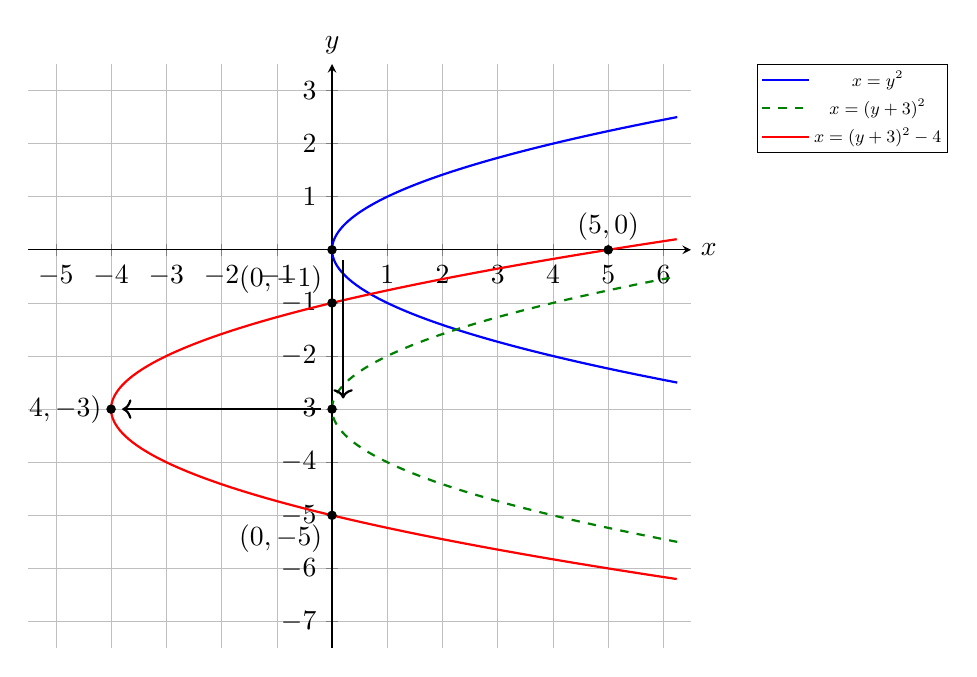
\begin{tikzpicture}
                \begin{axis}[
        axis lines = middle,
        xlabel = $x$,
        ylabel = {$y$},
        grid=both,
        grid style={line width=.1pt, draw=gray!10},
        major grid style={line width=.2pt,draw=gray!50},
        x label style={anchor=west}, % label x ke kanan
        y label style={anchor=south}, % label y ke atas
        samples=200,
        legend style={
                at={(1.1,1)},
                anchor=north west,
                font=\small,         % mengecilkan ukuran font
                row sep=1pt,         % jarak antar baris legend
                inner sep=1pt,       % margin dalam kotak legend
                nodes={scale=0.7}    % skalakan isi legend
            },
        xtick={-5,-4,...,6},
        ytick={-7,-6,...,3},
        xmin=-5.5, xmax=6.5,
        ymin=-7.5, ymax=3.5,
        width=10cm,
        height=9cm
    ]
\addplot[domain=-2.5:2.5, color=blue, thick] ({(x)*(x)},{x});
\addlegendentry{$x=y^2$}
\addplot[domain=-5.5:-0.5, color=green!50!black, thick, dashed] ({(x+3)*(x+3)},{x});
\addlegendentry{$x=(y+3)^2$}
\addplot[domain=-6.2:0.2, color=red, thick] ({(x+3)*(x+3)-4},{x});
\addlegendentry{$x=(y+3)^2-4$}
\draw[fill=black] (0,0) circle (1.5pt);
\draw[fill=black] (0,-3) circle (1.5pt);
\draw[fill=black] (-4,-3) circle (1.5pt) node[left] {$(-4,-3)$};
\draw[fill=black] (5,0) circle (1.5pt) node[above] {$(5,0)$};
\draw[fill=black] (0,-1) circle (1.5pt) node[above left] {$(0,-1)$};
\draw[fill=black] (0,-5) circle (1.5pt) node[below left] {$(0,-5)$};
\draw[->, thick] (0.2,-0.2) -- (0.2,-2.8);
\draw[->, thick] (-0.2,-3) -- (-3.8,-3);
\end{axis}
            \end{tikzpicture}
        \end{center}
        Jadi kurva $x = y^2 + 6y + 5$ adalah
        \[\colorlet{oldcolor}{.}
        \color{red}
        \setlength{\fboxrule}{1pt} \boxed{\color{oldcolor}\text{parabola } x=y^2 \text{ yang digeser 3 satuan ke bawah dan 4 satuan ke kiri}}\color{oldcolor}.\]
    }
    \end{jawab}
\end{enumerate}

\newpage

%%%%%%%%%%%%%%%%%%%%%%%%%%%%%%%%%%%%%%%%%%%%%%%%%%%%%%%%%%%%%%%%%%%%%%%%%%%%%%
% Kal-9
\kopsoal{Kal-9}{44-48}{T. Sistem Perkapalan, T. Kelautan, T. Komputer}{Senin, Rabu; 12.30-15.00}{3}
\begin{enumerate}
    \item Dapatkan penyelesaian dari $|x+1|=|2x-3|+1$.
    \begin{jawab}[definisi nilai mutlak, persamaan nilai mutlak, pembagian kasus]{~\\
        Ingat kembali definisi nilai mutlak, yaitu
        \begin{align*}
            |x+1| = \begin{cases}
                x+1, & x\geq -1\\
                -(x+1), & x<-1
            \end{cases}
            \quad\text{dan}\quad
            |2x-3| = \begin{cases}
                2x-3, & x\geq \frac{3}{2}\\
                -(2x-3), & x<\frac{3}{2}
            \end{cases}.
        \end{align*}
        Titik-titik batasnya adalah $\colorlet{oldcolor}{.}
        \color{blue}
        \setlength{\fboxrule}{1pt} \boxed{\color{oldcolor}x=-1}\color{oldcolor}$ dan $\colorlet{oldcolor}{.}
        \color{blue}
        \setlength{\fboxrule}{1pt} \boxed{\color{oldcolor}x=\frac{3}{2}}\color{oldcolor}$, sehingga garis bilangan terbagi menjadi tiga kasus.
        \begin{enumerate}
            \item[(i)] Jika $x<-1$, maka persamaan menjadi
            \begin{align*}
                -(x+1) = -(2x-3)+1 \iff -x-1 = -2x+4 \iff x = 5.
            \end{align*}
            Namun $x=5$ tidak memenuhi syarat $x<-1$, sehingga $\colorlet{oldcolor}{.}
        \color{blue}
        \setlength{\fboxrule}{1pt} \boxed{\color{oldcolor}\text{tidak ada solusi}}\color{oldcolor}$ pada kasus ini.
            \item[(ii)] Jika $-1\leq x<\frac{3}{2}$, maka persamaan menjadi
            \begin{align*}
                x+1 = -(2x-3)+1 \iff x+1 = -2x+4 \iff 3x = 3 \iff x=1.
            \end{align*}
            Karena $-1\leq 1<\frac{3}{2}$, maka $\colorlet{oldcolor}{.}
        \color{blue}
        \setlength{\fboxrule}{1pt} \boxed{\color{oldcolor}x=1}\color{oldcolor}$ memenuhi.
            \item[(iii)] Jika $x\geq\frac{3}{2}$, maka persamaan menjadi
            \begin{align*}
                x+1 = (2x-3)+1 \iff x+1 = 2x-2 \iff x=3.
            \end{align*}
            Karena $3\geq\frac{3}{2}$, maka $\colorlet{oldcolor}{.}
        \color{blue}
        \setlength{\fboxrule}{1pt} \boxed{\color{oldcolor}x=3}\color{oldcolor}$ memenuhi.
        \end{enumerate}
        Sebagai pengecekan, untuk $x=1$ diperoleh $|2|=2$ dan $|-1|+1=2$, sedangkan untuk $x=3$ diperoleh $|4|=4$ dan $|3|+1=4$. Jadi penyelesaiannya adalah $\colorlet{oldcolor}{.}
        \color{red}
        \setlength{\fboxrule}{1pt} \boxed{\color{oldcolor}x=1 \text{ atau } x=3}\color{oldcolor}$, atau ditulis $HP=\{1,3\}$.
    }
    \end{jawab}

    \item Diberikan titik $A(1,-2)$, $B(-1,3)$ dan $C(3,1)$.
    \begin{enumerate}
        \item Dapatkan persamaan garis yang melalui titik $A$ dan sejajar dengan garis yang melalui $B$ dan $C$.
        \item Dapatkan persamaan garis yang melalui titik $A$ dan tegak lurus dengan garis yang melalui $B$ dan $C$.
    \end{enumerate}
    \begin{jawab}[gradien garis, garis sejajar, garis tegak lurus, persamaan garis]{~\\
        Kemiringan garis yang melalui dua titik $(x_1,y_1)$ dan $(x_2,y_2)$ adalah $m = \frac{y_2 - y_1}{x_2 - x_1}$. Dengan substitusi $B(-1,3)$ dan $C(3,1)$, diperoleh
        \begin{align*}
            m_{BC} = \frac{1-3}{3-(-1)} = \frac{-2}{4} = \colorlet{oldcolor}{.}
        \color{blue}
        \setlength{\fboxrule}{1pt} \boxed{\color{oldcolor}-\frac{1}{2}}\color{oldcolor}.
        \end{align*}
        \begin{enumerate}
            \item Dua garis sejajar memiliki gradien yang sama, yaitu $\colorlet{oldcolor}{.}
        \color{blue}
        \setlength{\fboxrule}{1pt} \boxed{\color{oldcolor}m_1=m_2}\color{oldcolor}$, sehingga gradien garis yang dicari adalah $m=-\frac{1}{2}$. Garis tersebut melalui titik $A(1,-2)$, sehingga dengan rumus $y - y_1 = m(x - x_1)$ diperoleh
            \begin{align*}
                y - (-2) &= -\frac{1}{2}(x - 1)\\
                y + 2 &= -\frac{1}{2}x + \frac{1}{2}\\
                y &= -\frac{1}{2}x - \frac{3}{2}.
            \end{align*}
            Jadi persamaan garisnya adalah $\colorlet{oldcolor}{.}
        \color{red}
        \setlength{\fboxrule}{1pt} \boxed{\color{oldcolor}y = -\frac{1}{2}x - \frac{3}{2}}\color{oldcolor}$ atau $x+2y+3=0$.
            \item Dua garis saling tegak lurus jika $\colorlet{oldcolor}{.}
        \color{blue}
        \setlength{\fboxrule}{1pt} \boxed{\color{oldcolor}m_1\cdot m_2=-1}\color{oldcolor}$, sehingga gradien garis yang dicari memenuhi $-\frac{1}{2}\cdot m=-1$, yaitu $m=2$. Garis tersebut melalui titik $A(1,-2)$, sehingga
            \begin{align*}
                y - (-2) &= 2(x - 1)\\
                y + 2 &= 2x - 2\\
                y &= 2x - 4.
            \end{align*}
            Jadi persamaan garisnya adalah $\colorlet{oldcolor}{.}
        \color{red}
        \setlength{\fboxrule}{1pt} \boxed{\color{oldcolor}y = 2x - 4}\color{oldcolor}$ atau $2x-y-4=0$.
        \end{enumerate}
    }
    \end{jawab}

    \item Diberikan $f(x)=\sqrt[3]{x+2},\ x\geq -2$.
    \begin{enumerate}
        \item Dapatkan $f^{-1}(x)$ beserta domainnya.
        \item Sketsa $f(x)$ dan $f^{-1}(x)$ pada satu bidang koordinat.
    \end{enumerate}
    \begin{jawab}[fungsi invers, domain dan range, sketsa grafik fungsi invers]{
        \begin{enumerate}
            \item Untuk mendapatkan fungsi invers dari $f(x)$, kita misalkan $y=f(x)$, kemudian selesaikan sehingga terbentuk $x$ dalam fungsi $y$. Diperoleh
            \begin{align*}
                y &= \sqrt[3]{x+2}\\
                y^3 &= x+2\\
                x &= y^3 - 2.
            \end{align*}
            Dari sini didapatkan $x = f^{-1}(y) = y^3 - 2$. Dengan mengganti $y$ dengan $x$, diperoleh $f^{-1}(x) = x^3 - 2$.\\
            Selanjutnya, karena domain $f$ dibatasi pada $x\geq -2$, maka $x+2\geq 0$ sehingga $\sqrt[3]{x+2}\geq 0$, dan nilainya membesar tanpa batas. Jadi range dari $f$ adalah $R(f)=[0,\infty)$. Domain dari fungsi invers adalah range dari fungsi asli, yaitu $\colorlet{oldcolor}{.}
        \color{blue}
        \setlength{\fboxrule}{1pt} \boxed{\color{oldcolor}D(f^{-1}) = R(f) = [0, \infty)}\color{oldcolor}$, serta range dari fungsi invers adalah domain dari fungsi asli, yaitu $\colorlet{oldcolor}{.}
        \color{blue}
        \setlength{\fboxrule}{1pt} \boxed{\color{oldcolor}R(f^{-1}) = D(f) = [-2, \infty)}\color{oldcolor}$. Jadi fungsi inversnya adalah
            \begin{align*}
                \colorlet{oldcolor}{.}
        \color{red}
        \setlength{\fboxrule}{1pt} \boxed{\color{oldcolor}f^{-1}(x) = x^3 - 2,\quad D(f^{-1})=[0,\infty)}\color{oldcolor}.
            \end{align*}
            \item Grafik $f^{-1}$ merupakan pencerminan grafik $f$ terhadap garis $y=x$. Sebagai bantuan, grafik $f$ melalui titik $(-2,0)$, $(-1,1)$, dan $(6,2)$, sehingga grafik $f^{-1}$ melalui titik $(0,-2)$, $(1,-1)$, dan $(2,6)$. Sketsa grafiknya adalah sebagai berikut.
            \begin{center}
                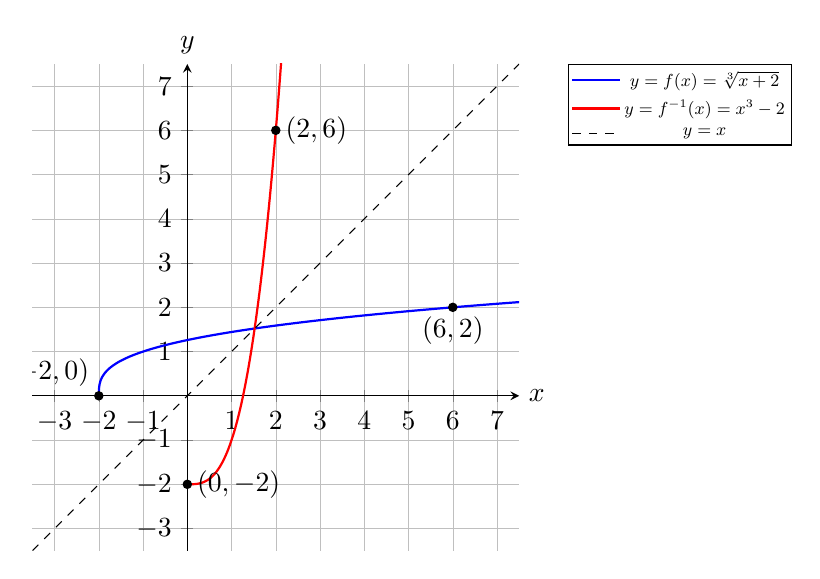
\begin{tikzpicture}
                    \begin{axis}[
        axis lines = middle,
        xlabel = $x$,
        ylabel = {$y$},
        grid=both,
        grid style={line width=.1pt, draw=gray!10},
        major grid style={line width=.2pt,draw=gray!50},
        x label style={anchor=west}, % label x ke kanan
        y label style={anchor=south}, % label y ke atas
        samples=200,
        legend style={
                at={(1.1,1)},
                anchor=north west,
                font=\small,         % mengecilkan ukuran font
                row sep=1pt,         % jarak antar baris legend
                inner sep=1pt,       % margin dalam kotak legend
                nodes={scale=0.7}    % skalakan isi legend
            },
        xtick={-3,-2,...,7},
        ytick={-3,-2,...,7},
        xmin=-3.5, xmax=7.5,
        ymin=-3.5, ymax=7.5,
        axis equal image,
        width=9cm
    ]
\addplot[domain=0:2.13, color=blue, thick, variable=\t] ({(\t)*(\t)*(\t)-2},{\t});
\addlegendentry{$y=f(x)=\sqrt[3]{x+2}$}
\addplot[domain=0:2.13, color=red, thick, variable=\t] ({\t},{(\t)*(\t)*(\t)-2});
\addlegendentry{$y=f^{-1}(x)=x^3-2$}
\addplot[domain=-3.5:7.5, color=black, dashed, samples=2] {x};
\addlegendentry{$y=x$}
\draw[fill=black] (-2,0) circle (1.5pt) node[above left] {$(-2,0)$};
\draw[fill=black] (6,2) circle (1.5pt) node[below] {$(6,2)$};
\draw[fill=black] (0,-2) circle (1.5pt) node[right] {$(0,-2)$};
\draw[fill=black] (2,6) circle (1.5pt) node[right] {$(2,6)$};
\end{axis}
                \end{tikzpicture}
            \end{center}
        \end{enumerate}
    }
    \end{jawab}

    \item Hitunglah $\displaystyle\lim_{y\to-\infty}\frac{3-2y}{\sqrt{5+9y^2}}$.
    \begin{jawab}[limit di tak hingga, bentuk akar, nilai mutlak]{~\\
        Diperhatikan bahwa jika $y\to-\infty$, pembilang dan penyebut sama-sama menuju tak hingga, sehingga diperoleh bentuk tak tentu $\frac{\infty}{\infty}$. Untuk menyelesaikannya, keluarkan $y^2$ dari dalam akar dengan mengingat bahwa $\colorlet{oldcolor}{.}
        \color{blue}
        \setlength{\fboxrule}{1pt} \boxed{\color{oldcolor}\sqrt{y^2}=|y|}\color{oldcolor}$, dan karena $y\to-\infty$ (yaitu $y<0$), maka $\colorlet{oldcolor}{.}
        \color{blue}
        \setlength{\fboxrule}{1pt} \boxed{\color{oldcolor}|y|=-y}\color{oldcolor}$. Diperoleh
        \begin{align*}
            \sqrt{5+9y^2} = \sqrt{y^2\left(\frac{5}{y^2}+9\right)} = |y|\sqrt{\frac{5}{y^2}+9} = -y\sqrt{\frac{5}{y^2}+9}.
        \end{align*}
        Dengan demikian,
        \begin{align*}
            \lim_{y\to-\infty}\frac{3-2y}{\sqrt{5+9y^2}} &= \lim_{y\to-\infty}\frac{3-2y}{-y\sqrt{\frac{5}{y^2}+9}}\\
            &= \lim_{y\to-\infty}\frac{-\frac{3}{y}+2}{\sqrt{\frac{5}{y^2}+9}}\\
            &= \frac{0+2}{\sqrt{0+9}}\\
            &= \colorlet{oldcolor}{.}
        \color{red}
        \setlength{\fboxrule}{1pt} \boxed{\color{oldcolor}\frac{2}{3}}\color{oldcolor}.
        \end{align*}
    }
    \end{jawab}

    \item Dapatkan persamaan garis singgung kurva $x^2+y+\dfrac{2y}{x}=\sqrt{x}+3$ di titik $(1,1)$.
    \begin{jawab}[diferensiasi implisit, aturan pembagian, persamaan garis singgung]{~\\
        Terlebih dahulu dicek bahwa titik $(1,1)$ terletak pada kurva, yaitu $1^2+1+\frac{2(1)}{1}=4$ dan $\sqrt{1}+3=4$. Selanjutnya, kita turunkan kedua ruas terhadap $x$, dengan mengingat bahwa $y$ adalah fungsi dari $x$. Dengan aturan pembagian, diperoleh
        \begin{align*}
            \colorlet{oldcolor}{.}
        \color{blue}
        \setlength{\fboxrule}{1pt} \boxed{\color{oldcolor}\frac{d}{dx}\left(\frac{2y}{x}\right) = \frac{2\frac{dy}{dx}\cdot x - 2y\cdot 1}{x^2} = \frac{2x\frac{dy}{dx} - 2y}{x^2}}\color{oldcolor}.
        \end{align*}
        Dengan demikian, diperoleh
        \begin{align*}
            2x + \frac{dy}{dx} + \frac{2x\frac{dy}{dx} - 2y}{x^2} = \frac{1}{2\sqrt{x}}.
        \end{align*}
        Selanjutnya, substitusi titik $(1,1)$ ke persamaan tersebut:
        \begin{align*}
            2(1) + \frac{dy}{dx} + \frac{2(1)\frac{dy}{dx} - 2(1)}{1^2} &= \frac{1}{2\sqrt{1}}\\
            2 + \frac{dy}{dx} + 2\frac{dy}{dx} - 2 &= \frac{1}{2}\\
            3\frac{dy}{dx} &= \frac{1}{2}\\
            \frac{dy}{dx}\bigg|_{(1,1)} &= \colorlet{oldcolor}{.}
        \color{blue}
        \setlength{\fboxrule}{1pt} \boxed{\color{oldcolor}\frac{1}{6}}\color{oldcolor}.
        \end{align*}
        Gradien garis singgung di titik $(1,1)$ adalah $m=\frac{1}{6}$. Dengan menggunakan persamaan garis $y - y_1 = m(x - x_1)$, di mana $(x_1,y_1)=(1,1)$, diperoleh
        \begin{align*}
            y - 1 &= \frac{1}{6}(x - 1)\\
            y &= \frac{1}{6}x + \frac{5}{6}.
        \end{align*}
        Jadi persamaan garis singgung di titik $(1,1)$ adalah $\colorlet{oldcolor}{.}
        \color{red}
        \setlength{\fboxrule}{1pt} \boxed{\color{oldcolor}y = \frac{1}{6}x + \frac{5}{6}}\color{oldcolor}$ atau $x-6y+5=0$.
    }
    \end{jawab}
\end{enumerate}

\newpage

%%%%%%%%%%%%%%%%%%%%%%%%%%%%%%%%%%%%%%%%%%%%%%%%%%%%%%%%%%%%%%%%%%%%%%%%%%%%%%
% Kal-11
\kopsoal{Kal-11}{51-54}{Biologi, Bioteknologi, Teknologi Informasi}{Senin, Rabu; 12.30-15.00}{3}
\begin{enumerate}
    \item \begin{enumerate}
        \item Definisikan $|x-1|$.
        \item Berdasarkan point (a) tersebut, tentukan semua nilai $x$ yang memenuhi pertidaksamaan
        \begin{align*}
            |x-1|\leq 5-2x.
        \end{align*}
    \end{enumerate}
    \begin{jawab}[definisi nilai mutlak, pertidaksamaan nilai mutlak]{
        \begin{enumerate}
            \item Ingat kembali definisi nilai mutlak, yaitu
            \begin{align*}
                |x-1| &= \begin{cases}
                    x-1, & x-1 \geq 0\\
                    -(x-1), & x-1 < 0
                \end{cases} \\
                &= \colorlet{oldcolor}{.}
        \color{red}
        \setlength{\fboxrule}{1pt} \boxed{\color{oldcolor}\begin{cases}
                    x-1, & x\geq 1\\
                    1-x, & x<1
                \end{cases}}\color{oldcolor}.
            \end{align*}
            \item Berdasarkan definisi tersebut, pertidaksamaan $|x-1|\leq 5-2x$ dapat ditulis menjadi dua kasus:
            \begin{enumerate}
                \item[(i)] Jika $x\geq 1$, maka pertidaksamaan menjadi $x-1\leq 5-2x$, yang dapat diselesaikan menjadi $3x\leq 6$ atau $x\leq 2$. Irisan dengan syarat $x\geq 1$ adalah $\colorlet{oldcolor}{.}
        \color{blue}
        \setlength{\fboxrule}{1pt} \boxed{\color{oldcolor}1\leq x\leq 2}\color{oldcolor}$.
                \item[(ii)] Jika $x<1$, maka pertidaksamaan menjadi $1-x\leq 5-2x$, yang dapat diselesaikan menjadi $x\leq 4$. Irisan dengan syarat $x<1$ adalah $\colorlet{oldcolor}{.}
        \color{blue}
        \setlength{\fboxrule}{1pt} \boxed{\color{oldcolor}x<1}\color{oldcolor}$.
            \end{enumerate}
            Dengan menggabungkan kedua kasus, semua nilai $x$ yang memenuhi pertidaksamaan tersebut adalah $(-\infty,1)\cup[1,2]$, yaitu $\colorlet{oldcolor}{.}
        \color{red}
        \setlength{\fboxrule}{1pt} \boxed{\color{oldcolor}x \leq 2}\color{oldcolor}$, atau dalam notasi interval $(-\infty,2]$.\\
            Sebagai pengecekan, untuk $x=2$ diperoleh $|1|=1\leq 5-4=1$, sedangkan untuk $x=3$ diperoleh $|2|=2\not\leq 5-6=-1$.
        \end{enumerate}
    }
    \end{jawab}

    \item \begin{enumerate}
        \item Tentukan jarak titik $(-3,4)$ dan $(5,-2)$.
        \item Tentukan persamaan lingkaran yang diameternya adalah ruas garis dari titik $(-3,4)$ ke $(5,-2)$.
    \end{enumerate}
    \begin{jawab}[jarak titik, titik tengah, persamaan lingkaran]{
        \begin{enumerate}
            \item Ingat kembali rumus jarak antara dua titik $(x_1,y_1)$ dan $(x_2,y_2)$, yaitu
            \begin{align*}
                d = \sqrt{(x_2-x_1)^2+(y_2-y_1)^2}.
            \end{align*}
            Dengan substitusi $(x_1,y_1)=(-3,4)$ dan $(x_2,y_2)=(5,-2)$, diperoleh
            \begin{align*}
                d = \sqrt{(5-(-3))^2+(-2-4)^2}= \sqrt{8^2+(-6)^2}= \sqrt{64+36}= \sqrt{100}= 10.
            \end{align*}
            Jadi jarak antara titik $(-3,4)$ dan $(5,-2)$ adalah $\colorlet{oldcolor}{.}
        \color{red}
        \setlength{\fboxrule}{1pt} \boxed{\color{oldcolor}d = 10}\color{oldcolor}$.
            \item Diketahui bahwa diameter lingkaran adalah ruas garis dari titik $(-3,4)$ ke $(5,-2)$, sehingga jari-jari lingkaran adalah setengah dari panjang diameter, yaitu
            \begin{align*}
                \colorlet{oldcolor}{.}
        \color{blue}
        \setlength{\fboxrule}{1pt} \boxed{\color{oldcolor}r = \frac{d}{2} = \frac{10}{2} = 5}\color{oldcolor}.
            \end{align*}
            Karena kedua titik tersebut merupakan ujung-ujung diameter, maka pusat lingkaran adalah titik tengah dari dua titik tersebut. Titik tengah $(a,b)$ dari dua titik $(x_1,y_1)$ dan $(x_2,y_2)$ adalah
            \begin{align*}
                (a,b) = \left(\frac{x_1+x_2}{2},\frac{y_1+y_2}{2}\right).
            \end{align*}
            Dengan substitusi $(x_1,y_1)=(-3,4)$ dan $(x_2,y_2)=(5,-2)$, diperoleh
            \begin{align*}
                (a,b) = \left(\frac{-3+5}{2}, \frac{4+(-2)}{2}\right) = \left(\frac{2}{2}, \frac{2}{2}\right) = \colorlet{oldcolor}{.}
        \color{blue}
        \setlength{\fboxrule}{1pt} \boxed{\color{oldcolor}(1,1)}\color{oldcolor}.
            \end{align*}
            Persamaan lingkaran dengan pusat $(a,b)$ dan jari-jari $r$ adalah
            \begin{align*}
                (x-a)^2 + (y-b)^2 = r^2.
            \end{align*}
            Dengan substitusi $(a,b)=(1,1)$ dan $r=5$, diperoleh persamaan lingkarannya adalah
            $$\colorlet{oldcolor}{.}
        \color{red}
        \setlength{\fboxrule}{1pt} \boxed{\color{oldcolor}(x-1)^2 + (y-1)^2 = 25}\color{oldcolor}.$$
            atau dalam bentuk umum $x^2+y^2-2x-2y-23=0$.
        \end{enumerate}
    }
    \end{jawab}

    \item Diberikan fungsi $f(x)=-\sqrt{|x^2-9|}$ dan $g(x)=\dfrac{1}{x^2-4}$.
    \begin{enumerate}
        \item Dapatkan domain $f$ dan $g$.
        \item Dapatkan $(g\circ f)(x)$ beserta domainnya.
    \end{enumerate}
    \begin{jawab}[domain fungsi, nilai mutlak, fungsi komposisi, domain fungsi komposisi]{
        \begin{enumerate}
            \item Diperhatikan bahwa $f(x)$ memuat akar kuadrat, sehingga syaratnya adalah ekspresi di dalam akar tak negatif, yaitu $|x^2-9|\geq 0$. Karena nilai mutlak selalu tak negatif, syarat ini berlaku untuk setiap bilangan real $x$. Jadi
            \begin{align*}
                \colorlet{oldcolor}{.}
        \color{red}
        \setlength{\fboxrule}{1pt} \boxed{\color{oldcolor}D(f)=\mathbb{R}}\color{oldcolor}.
            \end{align*}
            Selanjutnya, $g(x)$ merupakan fungsi rasional, sehingga syaratnya adalah $x^2-4=(x-2)(x+2)\neq 0$. Jadi
            \begin{align*}
                \colorlet{oldcolor}{.}
        \color{red}
        \setlength{\fboxrule}{1pt} \boxed{\color{oldcolor}D(g)=\{x\in\mathbb{R} : x\neq -2,~x\neq 2\}=\mathbb{R}\setminus\{-2,2\}}\color{oldcolor}.
            \end{align*}
            \item Diperhatikan bahwa $(f(x))^2 = \left(-\sqrt{|x^2-9|}\right)^2 = |x^2-9|$, sehingga
            \begin{align*}
                (g\circ f)(x) = g(f(x)) = \frac{1}{(f(x))^2-4} = \colorlet{oldcolor}{.}
        \color{red}
        \setlength{\fboxrule}{1pt} \boxed{\color{oldcolor}\frac{1}{|x^2-9|-4}}\color{oldcolor}.
            \end{align*}
            Domain dari fungsi komposisi $g\circ f$ adalah semua nilai $x$ pada domain $f$ sehingga nilai dari $f(x)$ berada pada domain $g$, yang dapat dirumuskan sebagai
            \begin{align*}
                \colorlet{oldcolor}{.}
        \color{blue}
        \setlength{\fboxrule}{1pt} \boxed{\color{oldcolor}D(g\circ f) = \{x \in D(f) : f(x) \in D(g)\} = \{x \in \mathbb{R} : f(x) \neq \pm 2\}}\color{oldcolor}.
            \end{align*}
            Karena $f(x)\leq 0$, maka $f(x)\neq 2$ selalu berlaku. Selanjutnya, $f(x)=-2$ jika dan hanya jika $\sqrt{|x^2-9|}=2$, yaitu $|x^2-9|=4$, sehingga
            \begin{align*}
                x^2-9=4 \quad\vee\quad x^2-9=-4 \iff x^2=13 \quad\vee\quad x^2=5 \iff x=\pm\sqrt{13} \quad\vee\quad x=\pm\sqrt{5}.
            \end{align*}
            Didapatkan
            \begin{align*}
                \colorlet{oldcolor}{.}
        \color{red}
        \setlength{\fboxrule}{1pt} \boxed{\color{oldcolor}D(g\circ f) = \mathbb{R}\setminus\left\{-\sqrt{13},-\sqrt{5},\sqrt{5},\sqrt{13}\right\}}\color{oldcolor}.
            \end{align*}
        \end{enumerate}
    }
    \end{jawab}

    \item Diberikan $f(x)=\begin{cases}
        k^2(x+1), & x\leq 1\\
        (3-k)x, & x>1
    \end{cases}$.\\
    Tentukan semua nilai $k$ yang memenuhi agar $\displaystyle\lim_{x\to 1}f(x)$ ada.
    \begin{jawab}[limit sepihak, fungsi sepotong-sepotong, persamaan kuadrat]{~\\
        Ingat kembali bahwa $\displaystyle\lim_{x\to a}f(x)$ ada jika dan hanya jika limit kiri dan limit kanannya ada dan bernilai sama, yaitu $\colorlet{oldcolor}{.}
        \color{blue}
        \setlength{\fboxrule}{1pt} \boxed{\color{oldcolor}\lim_{x \to a^-} f(x) = \lim_{x \to a^+} f(x)}\color{oldcolor}$. Untuk $x\to 1^-$ (yaitu $x<1$) digunakan rumus $k^2(x+1)$, dan untuk $x\to 1^+$ (yaitu $x>1$) digunakan rumus $(3-k)x$. Diperoleh
        \begin{align*}
            \lim_{x\to 1^-} f(x) = \lim_{x\to 1^-} k^2(x+1) = 2k^2 \quad\text{dan}\quad \lim_{x\to 1^+} f(x) = \lim_{x\to 1^+} (3-k)x = 3-k.
        \end{align*}
        Agar limitnya ada, haruslah
        \begin{align*}
            2k^2 &= 3-k\\
            2k^2+k-3 &= 0\\
            (2k+3)(k-1) &= 0,
        \end{align*}
        sehingga $k=-\frac{3}{2}$ atau $k=1$. Jadi semua nilai $k$ yang memenuhi adalah $\colorlet{oldcolor}{.}
        \color{red}
        \setlength{\fboxrule}{1pt} \boxed{\color{oldcolor}k=-\frac{3}{2} \text{ atau } k=1}\color{oldcolor}$.\\
        Sebagai pengecekan, untuk $k=1$ kedua limit sepihak bernilai $2$, sedangkan untuk $k=-\frac{3}{2}$ kedua limit sepihak bernilai $\frac{9}{2}$.
    }
    \end{jawab}

    \item Diketahui kurva $x^3+xy-y^2=1$.
    \begin{enumerate}
        \item Dapatkan $\dfrac{dy}{dx}$ dengan menggunakan turunan fungsi implisit.
        \item Dari (a) dapatkan persamaan garis singgung pada kurva tersebut di titik $(1,1)$.
    \end{enumerate}
    \begin{jawab}[turunan implisit, aturan perkalian, persamaan garis singgung]{
        \begin{enumerate}
            \item Kita turunkan kedua ruas persamaan $x^3+xy-y^2=1$ terhadap $x$, dengan mengingat bahwa $y$ adalah fungsi dari $x$ (yaitu $y=y(x)$). Dengan aturan perkalian, $\colorlet{oldcolor}{.}
        \color{blue}
        \setlength{\fboxrule}{1pt} \boxed{\color{oldcolor}\frac{d}{dx}(xy) = y + x\frac{dy}{dx}}\color{oldcolor}$, dan dengan aturan rantai, $\colorlet{oldcolor}{.}
        \color{blue}
        \setlength{\fboxrule}{1pt} \boxed{\color{oldcolor}\frac{d}{dx}(y^2) = 2y\frac{dy}{dx}}\color{oldcolor}$. Diperoleh
            \begin{align*}
                \frac{d}{dx}(x^3) + \frac{d}{dx}(xy) - \frac{d}{dx}(y^2) &= \frac{d}{dx}(1)\\
                3x^2 + y + x\frac{dy}{dx} - 2y\frac{dy}{dx} &= 0.
            \end{align*}
            Selanjutnya, kumpulkan semua suku yang mengandung $\frac{dy}{dx}$ di satu ruas:
            \begin{align*}
                x\frac{dy}{dx} - 2y\frac{dy}{dx} &= -3x^2 - y\\
                (x - 2y)\frac{dy}{dx} &= -3x^2 - y\\
                \frac{dy}{dx} &= \frac{-3x^2 - y}{x - 2y} = \frac{3x^2+y}{2y-x}.
            \end{align*}
            Jadi diperoleh $\colorlet{oldcolor}{.}
        \color{red}
        \setlength{\fboxrule}{1pt} \boxed{\color{oldcolor}\frac{dy}{dx} = \frac{3x^2 + y}{2y - x}}\color{oldcolor}$.
            \item Terlebih dahulu dicek bahwa titik $(1,1)$ terletak pada kurva, yaitu $1^3+1(1)-1^2=1$. Untuk mendapatkan gradien garis singgung di titik $(1,1)$, substitusi $x=1$ dan $y=1$ ke dalam turunan yang telah diperoleh:
            \begin{align*}
                m=\left.\frac{dy}{dx}\right|_{(1,1)} = \frac{3(1)^2 + 1}{2(1) - 1}= \frac{4}{1}= \colorlet{oldcolor}{.}
        \color{blue}
        \setlength{\fboxrule}{1pt} \boxed{\color{oldcolor}4}\color{oldcolor}.
            \end{align*}
            Dengan menggunakan persamaan garis $y - y_1 = m(x - x_1)$, di mana $(x_1,y_1)=(1,1)$ dan $m=4$, diperoleh:
            \begin{align*}
                y - 1 &= 4(x - 1)\\
                y &= 4x - 3.
            \end{align*}
            Jadi persamaan garis singgung di titik $(1,1)$ adalah $\colorlet{oldcolor}{.}
        \color{red}
        \setlength{\fboxrule}{1pt} \boxed{\color{oldcolor}y = 4x - 3}\color{oldcolor}$ atau $4x-y=3$.
        \end{enumerate}
    }
    \end{jawab}
\end{enumerate}

\newpage

%%%%%%%%%%%%%%%%%%%%%%%%%%%%%%%%%%%%%%%%%%%%%%%%%%%%%%%%%%%%%%%%%%%%%%%%%%%%%%
% Kal-12
\kopsoal{Kal-12}{55-60}{Aktuaria, Teknik Informatika, RPL, RKA}{Senin, Rabu; 12.30-15.00}{3}
\begin{enumerate}
    \item \begin{enumerate}
        \item Nyatakan pernyataan $\sqrt{(3x+2)^2}$ dalam bentuk nilai mutlak.
        \item Dapatkan semua nilai $x$ yang memenuhi persamaan $\sqrt{(3x+2)^2}=3x+2$.
    \end{enumerate}
    \begin{jawab}[definisi nilai mutlak, persamaan nilai mutlak]{
        \begin{enumerate}
            \item Ingat bahwa $\sqrt{x^2}=|x|$, sehingga diperoleh
            \begin{align*}
                \colorlet{oldcolor}{.}
        \color{red}
        \setlength{\fboxrule}{1pt} \boxed{\color{oldcolor}\sqrt{(3x+2)^2} = |3x+2|}\color{oldcolor}.
            \end{align*}
            \item Berdasarkan (a), persamaan yang diberikan menjadi
            \begin{align*}
                |3x+2| = 3x+2.
            \end{align*}
            Kemudian, pertimbangkan definisi nilai mutlak, yaitu
            \begin{align*}
                |3x+2| = \begin{cases}
                    3x+2, & 3x+2 \geq 0\\
                    -(3x+2), & 3x+2 < 0
                \end{cases}
            \end{align*}
            Berdasarkan definisi tersebut, didapatkan bahwa persamaan $|3x+2| = 3x+2$ berlaku jika $3x+2 \geq 0$, yang berarti $x \geq -\frac{2}{3}$. Untuk $3x+2<0$, persamaan menjadi $-(3x+2)=3x+2$, yaitu $3x+2=0$, yang bertentangan dengan $3x+2<0$. Jadi semua nilai $x$ yang memenuhi persamaan tersebut adalah $\colorlet{oldcolor}{.}
        \color{red}
        \setlength{\fboxrule}{1pt} \boxed{\color{oldcolor}x \geq -\frac{2}{3}}\color{oldcolor}$, atau dalam notasi interval $\left[-\frac{2}{3},\infty\right)$.
        \end{enumerate}
    }
    \end{jawab}

    \item Diberikan fungsi $f(x)=\sqrt{x+3}$.
    \begin{enumerate}
        \item Tentukan domain dan range dari fungsi $f(x)$.
        \item Tentukan $f^{-1}(x)$, domain dan range dari $f^{-1}(x)$.
    \end{enumerate}
    \begin{jawab}[domain dan range fungsi, fungsi invers]{
        \begin{enumerate}
            \item Diperhatikan bahwa $f(x)$ memuat akar kuadrat, sehingga domainnya adalah semua bilangan real yang membuat ekspresi di dalam akar kuadrat tak negatif. Jadi
            \begin{align*}
                \colorlet{oldcolor}{.}
        \color{red}
        \setlength{\fboxrule}{1pt} \boxed{\color{oldcolor}D(f)=\{x \in \mathbb{R} : x+3 \geq 0\} = [-3, \infty)}\color{oldcolor}.
            \end{align*}
            Selanjutnya, karena $f(x)$ merupakan fungsi akar kuadrat, maka nilainya selalu tak negatif, dan untuk $x$ yang membesar dari $-3$, nilai $\sqrt{x+3}$ membesar dari $0$ tanpa batas. Jadi
            \begin{align*}
                \colorlet{oldcolor}{.}
        \color{red}
        \setlength{\fboxrule}{1pt} \boxed{\color{oldcolor}R(f)=\{y \in \mathbb{R} : y \geq 0\} = [0, \infty)}\color{oldcolor}.
            \end{align*}
            \item Untuk mendapatkan fungsi invers dari $f(x)$, kita misalkan $y=f(x)$, kemudian selesaikan sehingga terbentuk $x$ dalam fungsi $y$. Diperoleh
            \begin{align*}
                y &= f(x) = \sqrt{x+3}\\
                y^2 &= x+3\\
                x &= y^2 - 3.
            \end{align*}
            Dari sini didapatkan $x = f^{-1}(y) = y^2 - 3$. Dengan mengganti $y$ dengan $x$, diperoleh
            \begin{align*}
                f^{-1}(x) = x^2 - 3.
            \end{align*}
            Selanjutnya, domain dari fungsi invers adalah range dari fungsi asli, yaitu $\colorlet{oldcolor}{.}
        \color{blue}
        \setlength{\fboxrule}{1pt} \boxed{\color{oldcolor}D(f^{-1}) = R(f) = [0, \infty)}\color{oldcolor}$, serta range dari fungsi invers adalah domain dari fungsi asli, yaitu $\colorlet{oldcolor}{.}
        \color{blue}
        \setlength{\fboxrule}{1pt} \boxed{\color{oldcolor}R(f^{-1}) = D(f) = [-3, \infty)}\color{oldcolor}$. Jadi fungsi inversnya adalah
        \begin{align*}
            \colorlet{oldcolor}{.}
        \color{red}
        \setlength{\fboxrule}{1pt} \boxed{\color{oldcolor}f^{-1}(x) = x^2 - 3,\quad x\geq 0}\color{oldcolor}.
        \end{align*}
        \end{enumerate}
    }
    \end{jawab}

    \item Diberikan persamaan separuh lingkaran
    \begin{align*}
        x=-2-\sqrt{-y^2+4y+12}.
    \end{align*}
    \begin{enumerate}
        \item Dapatkan pusat dan jari-jari lingkaran.
        \item Sketsa grafiknya.
    \end{enumerate}
    \begin{jawab}[persamaan lingkaran, pusat dan jari-jari lingkaran, sketsa grafik]{
        \begin{enumerate}
            \item Diperhatikan bahwa persamaan tersebut dapat ditulis ulang menjadi
            \begin{align*}
                x+2 &= -\sqrt{-y^2+4y+12}\\
                (x+2)^2 &= -y^2+4y+12\\
                (x+2)^2 + y^2 - 4y - 12 &= 0\\
                (x+2)^2 + (y^2 - 4y + 4) - 4 - 12 &= 0\\
                (x+2)^2 + (y-2)^2 &= 16.
            \end{align*}
            Dari persamaan tersebut, dapat dilihat bahwa pusat lingkaran adalah $(-2,2)$ dan jari-jari lingkaran adalah $\sqrt{16} = 4$. Jadi pusat dan jari-jari lingkaran adalah $\colorlet{oldcolor}{.}
        \color{red}
        \setlength{\fboxrule}{1pt} \boxed{\color{oldcolor}\text{Pusat: }(-2,2),~\text{Jari-jari: }4}\color{oldcolor}$.
            \item Diperhatikan bahwa pada persamaan $x=-2-\sqrt{-y^2+4y+12}$ berlaku $x+2=-\sqrt{-y^2+4y+12}\leq 0$, artinya $\colorlet{oldcolor}{.}
        \color{blue}
        \setlength{\fboxrule}{1pt} \boxed{\color{oldcolor}x\leq -2}\color{oldcolor}$. Sehingga grafik separuh lingkaran yang diberikan dalam soal merupakan bagian kiri dari lingkaran $(x+2)^2+(y-2)^2=16$, dengan ujung-ujung $(-2,-2)$ dan $(-2,6)$ serta titik paling kiri $(-6,2)$. Sketsa grafiknya adalah sebagai berikut:
            \begin{center}
                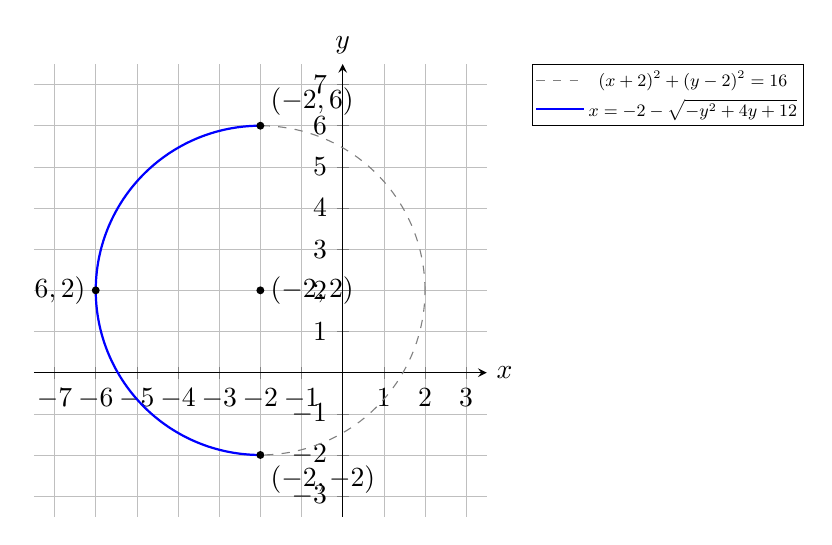
\begin{tikzpicture}
                   \begin{axis}[
        axis lines = middle,
        xlabel = $x$,
        ylabel = {$y$},
        grid=both,
        grid style={line width=.1pt, draw=gray!10},
        major grid style={line width=.2pt,draw=gray!50},
        x label style={anchor=west}, % label x ke kanan
        y label style={anchor=south}, % label y ke atas
        samples=200,
        legend style={
                at={(1.1,1)},
                anchor=north west,
                font=\small,         % mengecilkan ukuran font
                row sep=1pt,         % jarak antar baris legend
                inner sep=1pt,       % margin dalam kotak legend
                nodes={scale=0.7}    % skalakan isi legend
            },
        xtick={-7,-6,...,3},
        ytick={-3,-2,...,7},
        xmin=-7.5, xmax=3.5,
        ymin=-3.5, ymax=7.5,
        axis equal image,
        width=8.5cm
    ]
\addplot[domain=0:360, color=gray, dashed] ({-2+4*cos(x)}, {2+4*sin(x)});
\addlegendentry{$(x+2)^2+(y-2)^2=16$}
\addplot[domain=90:270, color=blue, thick] ({-2+4*cos(x)}, {2+4*sin(x)});
\addlegendentry{$x=-2-\sqrt{-y^2+4y+12}$}
\draw[fill=black, thick] (-2,2) circle (1pt) node[right] {$(-2,2)$};
\draw[fill=black, thick] (-2,-2) circle (1pt) node[below right] {$(-2,-2)$};
\draw[fill=black, thick] (-2,6) circle (1pt) node[above right] {$(-2,6)$};
\draw[fill=black, thick] (-6,2) circle (1pt) node[left] {$(-6,2)$};
\end{axis}
                \end{tikzpicture}
            \end{center}
            Grafik yang dimaksud adalah busur yang berwarna biru (setengah lingkaran bagian kiri).
        \end{enumerate}
    }
    \end{jawab}

    \item Diberikan fungsi $f(x)=\dfrac{9-x^2}{3-|x|}$.
    \begin{enumerate}
        \item Nyatakan fungsi $f(x)$ dalam bentuk fungsi sepotong-sepotong.
        \item Selidiki apakah $f(x)$ memiliki titik diskontinu.
        \item Jika memiliki titik diskontinu, apakah titik diskontinu dapat dihilangkan?
    \end{enumerate}
    \begin{jawab}[definisi nilai mutlak, fungsi sepotong-sepotong, kekontinuan, diskontinuitas yang dapat dihapus]{
        \begin{enumerate}
            \item Fungsi $f$ terdefinisi jika $3-|x|\neq 0$, yaitu $x\neq\pm 3$. Ingat kembali definisi nilai mutlak, yaitu $|x|=x$ untuk $x\geq 0$ dan $|x|=-x$ untuk $x<0$. Diperoleh
            \begin{itemize}
                \item Untuk $x\geq 0$ dan $x\neq 3$: $\displaystyle f(x) = \frac{9-x^2}{3-x} = \frac{(3-x)(3+x)}{3-x} = 3+x$.
                \item Untuk $x<0$ dan $x\neq -3$: $\displaystyle f(x) = \frac{9-x^2}{3+x} = \frac{(3-x)(3+x)}{3+x} = 3-x$.
            \end{itemize}
            Jadi
            \begin{align*}
                \colorlet{oldcolor}{.}
        \color{red}
        \setlength{\fboxrule}{1pt} \boxed{\color{oldcolor}f(x) = \begin{cases}
                    3-x, & x<0,~x\neq -3\\
                    3+x, & x\geq 0,~x\neq 3
                \end{cases}}\color{oldcolor}.
            \end{align*}
            \item Pada interval-interval $(-\infty,-3)$, $(-3,0)$, $(0,3)$, dan $(3,\infty)$, fungsi $f$ berupa fungsi linear sehingga kontinu. Titik-titik yang perlu diselidiki adalah $x=0$ (titik pergantian rumus) serta $x=-3$ dan $x=3$ (titik yang membuat penyebut nol).
            \begin{itemize}
                \item Di $x=0$: $f(0)=3+0=3$, $\displaystyle\lim_{x\to 0^-}(3-x)=3$, dan $\displaystyle\lim_{x\to 0^+}(3+x)=3$, sehingga $\displaystyle\lim_{x\to 0}f(x)=3=f(0)$. Jadi $f$ $\colorlet{oldcolor}{.}
        \color{blue}
        \setlength{\fboxrule}{1pt} \boxed{\color{oldcolor}\text{kontinu di } x=0}\color{oldcolor}$.
                \item Di $x=3$: $f(3)$ tidak terdefinisi karena penyebutnya nol, sehingga $f$ $\colorlet{oldcolor}{.}
        \color{blue}
        \setlength{\fboxrule}{1pt} \boxed{\color{oldcolor}\text{diskontinu di } x=3}\color{oldcolor}$.
                \item Di $x=-3$: $f(-3)$ tidak terdefinisi karena penyebutnya nol, sehingga $f$ $\colorlet{oldcolor}{.}
        \color{blue}
        \setlength{\fboxrule}{1pt} \boxed{\color{oldcolor}\text{diskontinu di } x=-3}\color{oldcolor}$.
            \end{itemize}
            Jadi $f(x)$ memiliki titik diskontinu, yaitu di $\colorlet{oldcolor}{.}
        \color{red}
        \setlength{\fboxrule}{1pt} \boxed{\color{oldcolor}x=-3 \text{ dan } x=3}\color{oldcolor}$.
            \item Suatu titik diskontinu $x=a$ dapat dihilangkan jika $\displaystyle\lim_{x\to a}f(x)$ ada. Diperhatikan bahwa
            \begin{align*}
                \lim_{x\to 3}f(x) = \lim_{x\to 3}(3+x) = 6 \quad\text{dan}\quad \lim_{x\to -3}f(x) = \lim_{x\to -3}(3-x) = 6.
            \end{align*}
            Karena kedua limit tersebut ada, maka $\colorlet{oldcolor}{.}
        \color{red}
        \setlength{\fboxrule}{1pt} \boxed{\color{oldcolor}\text{kedua titik diskontinu dapat dihilangkan}}\color{oldcolor}$, yaitu dengan mendefinisikan $f(-3)=6$ dan $f(3)=6$. Dengan definisi tersebut, $f(x)=3+|x|$ untuk setiap $x\in\mathbb{R}$. Sketsa grafik $f$ (sebelum titik diskontinunya dihilangkan) adalah sebagai berikut:
            \begin{center}
                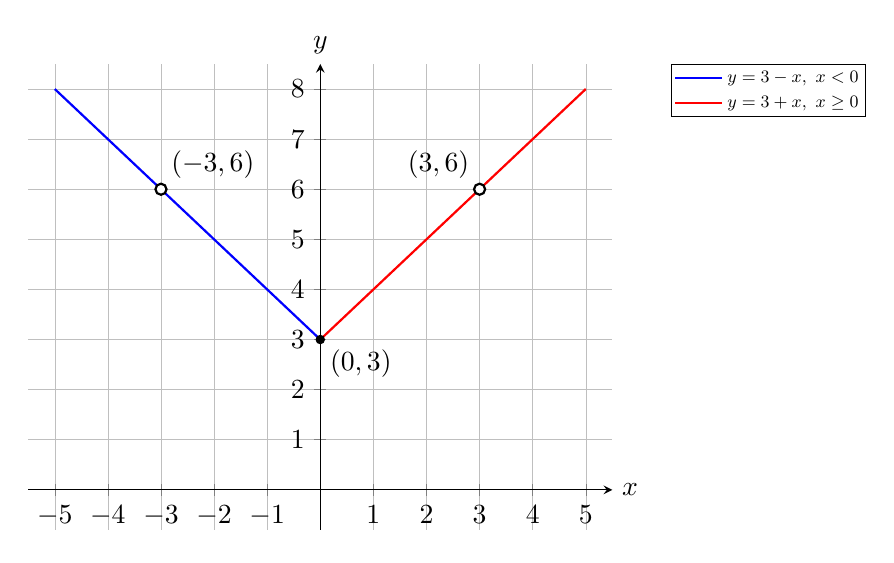
\begin{tikzpicture}
                    \begin{axis}[
        axis lines = middle,
        xlabel = $x$,
        ylabel = {$y$},
        grid=both,
        grid style={line width=.1pt, draw=gray!10},
        major grid style={line width=.2pt,draw=gray!50},
        x label style={anchor=west}, % label x ke kanan
        y label style={anchor=south}, % label y ke atas
        samples=200,
        legend style={
                at={(1.1,1)},
                anchor=north west,
                font=\small,         % mengecilkan ukuran font
                row sep=1pt,         % jarak antar baris legend
                inner sep=1pt,       % margin dalam kotak legend
                nodes={scale=0.7}    % skalakan isi legend
            },
        xtick={-5,-4,...,5},
        ytick={0,1,...,8},
        xmin=-5.5, xmax=5.5,
        ymin=-0.8, ymax=8.5,
        width=9cm,
        height=7.5cm
    ]
\addplot[domain=-5:0, color=blue, thick, samples=2] {3-x};
\addlegendentry{$y=3-x,\ x<0$}
\addplot[domain=0:5, color=red, thick, samples=2] {3+x};
\addlegendentry{$y=3+x,\ x\geq 0$}
\draw[fill=white, thick] (-3,6) circle (2pt) node[above right] {$(-3,6)$};
\draw[fill=white, thick] (3,6) circle (2pt) node[above left] {$(3,6)$};
\draw[fill=black] (0,3) circle (1.5pt) node[below right] {$(0,3)$};
\end{axis}
                \end{tikzpicture}
            \end{center}
        \end{enumerate}
    }
    \end{jawab}

    \item Diketahui fungsi $f(x)=\left(x^2-\dfrac{4}{x}\right)^{3/2}$. Dapatkan $f'(2)$.
    \begin{jawab}[turunan fungsi, aturan rantai]{~\\
        Ingat kembali aturan rantai untuk turunan fungsi, yaitu
        \[
        \colorlet{oldcolor}{.}
        \color{blue}
        \setlength{\fboxrule}{1pt} \boxed{\color{oldcolor}\frac{d}{dx}[h(g(x))] = h'(g(x)) \cdot g'(x)}\color{oldcolor}.
        \]
        Dapat dimisalkan $\colorlet{oldcolor}{.}
        \color{blue}
        \setlength{\fboxrule}{1pt} \boxed{\color{oldcolor}u=g(x) = x^2-\frac{4}{x}}\color{oldcolor}$ sehingga $\colorlet{oldcolor}{.}
        \color{blue}
        \setlength{\fboxrule}{1pt} \boxed{\color{oldcolor}h(u) = u^{3/2}}\color{oldcolor}$, dan diperoleh
        \begin{align*}
            \colorlet{oldcolor}{.}
        \color{blue}
        \setlength{\fboxrule}{1pt} \boxed{\color{oldcolor}h'(u) = \frac{3}{2}u^{1/2}}\color{oldcolor} \quad \text{dan}\quad
        \colorlet{oldcolor}{.}
        \color{blue}
        \setlength{\fboxrule}{1pt} \boxed{\color{oldcolor}g'(x) = 2x+\frac{4}{x^2}}\color{oldcolor}.
        \end{align*}
        Dengan demikian, diperoleh
        \begin{align*}
            f'(x) &=
            h'(u) \cdot g'(x)\\
            &= \frac{3}{2}u^{1/2} \cdot \left(2x+\frac{4}{x^2}\right)\\
            &= \colorlet{oldcolor}{.}
        \color{blue}
        \setlength{\fboxrule}{1pt} \boxed{\color{oldcolor}\frac{3}{2}\left(x^2-\frac{4}{x}\right)^{1/2} \left(2x+\frac{4}{x^2}\right)}\color{oldcolor}.
        \end{align*}
        Selanjutnya, substitusi $x=2$ ke dalam $f'(x)$, diperoleh
        \begin{align*}
            f'(2) &= \frac{3}{2}\left(4-\frac{4}{2}\right)^{1/2} \left(4+\frac{4}{4}\right)\\
            &= \frac{3}{2}\left(2\right)^{1/2} \left(5\right)\\
            &= \colorlet{oldcolor}{.}
        \color{red}
        \setlength{\fboxrule}{1pt} \boxed{\color{oldcolor}\frac{15}{2}\sqrt{2}}\color{oldcolor}.
        \end{align*}
    }
    \end{jawab}
\end{enumerate}

\newpage

%%%%%%%%%%%%%%%%%%%%%%%%%%%%%%%%%%%%%%%%%%%%%%%%%%%%%%%%%%%%%%%%%%%%%%%%%%%%%%
% Kal-7
\kopsoal{Kal-7}{32-37}{T. Sipil, T. Geomatika, T. Geofisika, T. Pertambangan}{Senin, Rabu; 15.30-17.10}{4}
\begin{enumerate}
    \item \begin{enumerate}
        \item Definisikan $|x+2|$.
        \item Berdasarkan point (a) tersebut, tentukan semua nilai $x$ yang memenuhi pertidaksamaan
        \begin{align*}
            |x+2|\leq 3x-2.
        \end{align*}
    \end{enumerate}
    \begin{jawab}[definisi nilai mutlak, pertidaksamaan nilai mutlak]{
        \begin{enumerate}
            \item Ingat kembali definisi nilai mutlak, yaitu
            \begin{align*}
                |x+2| &= \begin{cases}
                    x+2, & x+2 \geq 0\\
                    -(x+2), & x+2 < 0
                \end{cases} \\
                &= \colorlet{oldcolor}{.}
        \color{red}
        \setlength{\fboxrule}{1pt} \boxed{\color{oldcolor}\begin{cases}
                    x+2, & x\geq -2\\
                    -x-2, & x<-2
                \end{cases}}\color{oldcolor}.
            \end{align*}
            \item Berdasarkan definisi tersebut, pertidaksamaan $|x+2|\leq 3x-2$ dapat ditulis menjadi dua kasus:
            \begin{enumerate}
                \item[(i)] Jika $x\geq -2$, maka pertidaksamaan menjadi $x+2\leq 3x-2$, yang dapat diselesaikan menjadi $4\leq 2x$ atau $x\geq 2$. Irisan dengan syarat $x\geq -2$ adalah $\colorlet{oldcolor}{.}
        \color{blue}
        \setlength{\fboxrule}{1pt} \boxed{\color{oldcolor}x\geq 2}\color{oldcolor}$.
                \item[(ii)] Jika $x<-2$, maka pertidaksamaan menjadi $-x-2\leq 3x-2$, yang dapat diselesaikan menjadi $0\leq 4x$ atau $x\geq 0$. Namun, karena kita berada pada kasus $x<-2$, $\colorlet{oldcolor}{.}
        \color{blue}
        \setlength{\fboxrule}{1pt} \boxed{\color{oldcolor}\text{tidak ada solusi}}\color{oldcolor}$ pada kasus ini.
            \end{enumerate}
            Dengan menggabungkan kedua kasus, semua nilai $x$ yang memenuhi pertidaksamaan tersebut adalah $\colorlet{oldcolor}{.}
        \color{red}
        \setlength{\fboxrule}{1pt} \boxed{\color{oldcolor}x \geq 2}\color{oldcolor}$, atau dalam notasi interval $[2,\infty)$.
        \end{enumerate}
    }
    \end{jawab}

    \item \begin{enumerate}
        \item Tentukan jarak titik $(-2,1)$ dan $(4,9)$.
        \item Tentukan persamaan lingkaran yang diameternya adalah ruas garis dari titik $(-2,1)$ ke $(4,9)$.
    \end{enumerate}
    \begin{jawab}[jarak titik, titik tengah, persamaan lingkaran]{
        \begin{enumerate}
            \item Ingat kembali rumus jarak antara dua titik $(x_1,y_1)$ dan $(x_2,y_2)$, yaitu
            \begin{align*}
                d = \sqrt{(x_2-x_1)^2+(y_2-y_1)^2}.
            \end{align*}
            Dengan substitusi $(x_1,y_1)=(-2,1)$ dan $(x_2,y_2)=(4,9)$, diperoleh
            \begin{align*}
                d = \sqrt{(4-(-2))^2+(9-1)^2}= \sqrt{6^2+8^2}= \sqrt{36+64}= \sqrt{100}= 10.
            \end{align*}
            Jadi jarak antara titik $(-2,1)$ dan $(4,9)$ adalah $\colorlet{oldcolor}{.}
        \color{red}
        \setlength{\fboxrule}{1pt} \boxed{\color{oldcolor}d = 10}\color{oldcolor}$.
            \item Diketahui bahwa diameter lingkaran adalah ruas garis dari titik $(-2,1)$ ke $(4,9)$, sehingga jari-jari lingkaran adalah setengah dari panjang diameter, yaitu
            \begin{align*}
                \colorlet{oldcolor}{.}
        \color{blue}
        \setlength{\fboxrule}{1pt} \boxed{\color{oldcolor}r = \frac{d}{2} = \frac{10}{2} = 5}\color{oldcolor}.
            \end{align*}
            Karena kedua titik tersebut merupakan ujung-ujung diameter, maka pusat lingkaran adalah titik tengah dari dua titik tersebut. Titik tengah $(a,b)$ dari dua titik $(x_1,y_1)$ dan $(x_2,y_2)$ adalah
            \begin{align*}
                (a,b) = \left(\frac{x_1+x_2}{2},\frac{y_1+y_2}{2}\right).
            \end{align*}
            Dengan substitusi $(x_1,y_1)=(-2,1)$ dan $(x_2,y_2)=(4,9)$, diperoleh
            \begin{align*}
                (a,b) = \left(\frac{-2+4}{2}, \frac{1+9}{2}\right) = \left(\frac{2}{2}, \frac{10}{2}\right) = \colorlet{oldcolor}{.}
        \color{blue}
        \setlength{\fboxrule}{1pt} \boxed{\color{oldcolor}(1,5)}\color{oldcolor}.
            \end{align*}
            Persamaan lingkaran dengan pusat $(a,b)$ dan jari-jari $r$ adalah
            \begin{align*}
                (x-a)^2 + (y-b)^2 = r^2.
            \end{align*}
            Dengan substitusi $(a,b)=(1,5)$ dan $r=5$, diperoleh persamaan lingkarannya adalah
            $$\colorlet{oldcolor}{.}
        \color{red}
        \setlength{\fboxrule}{1pt} \boxed{\color{oldcolor}(x-1)^2 + (y-5)^2 = 25}\color{oldcolor}.$$
            atau dalam bentuk umum $x^2+y^2-2x-10y+1=0$.
        \end{enumerate}
    }
    \end{jawab}

    \item Diberikan suatu fungsi $f(x)=3-\sqrt{9-x^2}$ dengan domain $f$ adalah $[a,3]$.
    \begin{enumerate}
        \item Tentukan nilai terkecil $a$ agar $f^{-1}(x)$ ada.
        \item Dapatkan $f^{-1}(x)$.
        \item Sketsa grafik $f(x)$ dan $f^{-1}(x)$ pada satu bidang koordinat.
    \end{enumerate}
    \begin{jawab}[fungsi satu-satu, setengah lingkaran, fungsi invers, sketsa grafik fungsi invers]{
        \begin{enumerate}
            \item Suatu fungsi mempunyai invers jika fungsi tersebut satu-satu (injektif). Diperhatikan bahwa jika $y=3-\sqrt{9-x^2}$, maka $3-y=\sqrt{9-x^2}\geq 0$ dan
            \begin{align*}
                (3-y)^2 = 9-x^2 \iff \colorlet{oldcolor}{.}
        \color{blue}
        \setlength{\fboxrule}{1pt} \boxed{\color{oldcolor}x^2+(y-3)^2=9}\color{oldcolor},\quad y\leq 3,
            \end{align*}
            sehingga grafik $f$ adalah setengah lingkaran bagian bawah dengan pusat $(0,3)$ dan jari-jari $3$. Grafik ini turun pada $[-3,0]$ dan naik pada $[0,3]$, sehingga jika domainnya memuat titik di kiri dan kanan $x=0$, fungsi $f$ tidak satu-satu (misalnya $f(-3)=f(3)=3$). Agar $f$ satu-satu pada $[a,3]$, haruslah $a\geq 0$. Jadi nilai terkecil $a$ adalah $\colorlet{oldcolor}{.}
        \color{red}
        \setlength{\fboxrule}{1pt} \boxed{\color{oldcolor}a=0}\color{oldcolor}$.
            \item Misalkan $y=f(x)$ dengan $x\in[0,3]$, kemudian selesaikan sehingga terbentuk $x$ dalam fungsi $y$. Diperoleh
            \begin{align*}
                y &= 3-\sqrt{9-x^2}\\
                \sqrt{9-x^2} &= 3-y\\
                9-x^2 &= (3-y)^2\\
                x^2 &= 9-(3-y)^2 = 6y-y^2\\
                x &= \sqrt{6y-y^2} \quad (\text{karena } x\geq 0).
            \end{align*}
            Dari sini didapatkan $x = f^{-1}(y) = \sqrt{6y-y^2}$. Dengan mengganti $y$ dengan $x$, diperoleh
            \begin{align*}
                \colorlet{oldcolor}{.}
        \color{red}
        \setlength{\fboxrule}{1pt} \boxed{\color{oldcolor}f^{-1}(x) = \sqrt{6x-x^2}}\color{oldcolor}.
            \end{align*}
            Pada domain $[0,3]$, fungsi $f$ naik dari $f(0)=0$ sampai $f(3)=3$, sehingga $R(f)=[0,3]$. Akibatnya, $D(f^{-1})=R(f)=[0,3]$ dan $R(f^{-1})=D(f)=[0,3]$.
            \item Grafik $f$ adalah seperempat lingkaran berpusat di $(0,3)$ dan berjari-jari $3$ dari titik $(0,0)$ ke $(3,3)$. Grafik $f^{-1}$ merupakan pencerminan grafik $f$ terhadap garis $y=x$, yaitu seperempat lingkaran $(x-3)^2+y^2=9$ yang berpusat di $(3,0)$, juga dari titik $(0,0)$ ke $(3,3)$. Sketsa grafiknya adalah sebagai berikut.
            \begin{center}
                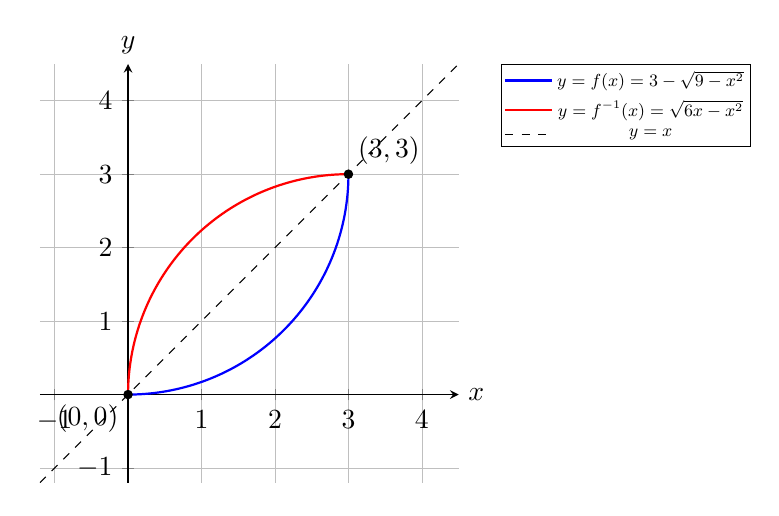
\begin{tikzpicture}
                    \begin{axis}[
        axis lines = middle,
        xlabel = $x$,
        ylabel = {$y$},
        grid=both,
        grid style={line width=.1pt, draw=gray!10},
        major grid style={line width=.2pt,draw=gray!50},
        x label style={anchor=west}, % label x ke kanan
        y label style={anchor=south}, % label y ke atas
        samples=200,
        legend style={
                at={(1.1,1)},
                anchor=north west,
                font=\small,         % mengecilkan ukuran font
                row sep=1pt,         % jarak antar baris legend
                inner sep=1pt,       % margin dalam kotak legend
                nodes={scale=0.7}    % skalakan isi legend
            },
        xtick={-1,0,...,4},
        ytick={-1,0,...,4},
        xmin=-1.2, xmax=4.5,
        ymin=-1.2, ymax=4.5,
        axis equal image,
        width=8cm
    ]
\addplot[domain=-90:0, color=blue, thick] ({3*cos(x)}, {3+3*sin(x)});
\addlegendentry{$y=f(x)=3-\sqrt{9-x^2}$}
\addplot[domain=90:180, color=red, thick] ({3+3*cos(x)}, {3*sin(x)});
\addlegendentry{$y=f^{-1}(x)=\sqrt{6x-x^2}$}
\addplot[domain=-1.2:4.5, color=black, dashed, samples=2] {x};
\addlegendentry{$y=x$}
\draw[fill=black] (0,0) circle (1.5pt) node[below left] {$(0,0)$};
\draw[fill=black] (3,3) circle (1.5pt) node[above right] {$(3,3)$};
\end{axis}
                \end{tikzpicture}
            \end{center}
        \end{enumerate}
    }
    \end{jawab}

    \item Hitunglah $\displaystyle\lim_{x\to-\infty}\frac{\sqrt{9x^2+1}}{2x-5}$.
    \begin{jawab}[limit di tak hingga, bentuk akar, nilai mutlak]{~\\
        Diperhatikan bahwa jika $x\to-\infty$, diperoleh bentuk tak tentu $\frac{\infty}{-\infty}$. Untuk menyelesaikannya, keluarkan $x^2$ dari dalam akar dengan mengingat bahwa $\colorlet{oldcolor}{.}
        \color{blue}
        \setlength{\fboxrule}{1pt} \boxed{\color{oldcolor}\sqrt{x^2}=|x|}\color{oldcolor}$, dan karena $x\to-\infty$ (yaitu $x<0$), maka $\colorlet{oldcolor}{.}
        \color{blue}
        \setlength{\fboxrule}{1pt} \boxed{\color{oldcolor}|x|=-x}\color{oldcolor}$. Diperoleh
        \begin{align*}
            \sqrt{9x^2+1} = \sqrt{x^2\left(9+\frac{1}{x^2}\right)} = |x|\sqrt{9+\frac{1}{x^2}} = -x\sqrt{9+\frac{1}{x^2}}.
        \end{align*}
        Dengan demikian,
        \begin{align*}
            \lim_{x\to-\infty}\frac{\sqrt{9x^2+1}}{2x-5} &= \lim_{x\to-\infty}\frac{-x\sqrt{9+\frac{1}{x^2}}}{x\left(2-\frac{5}{x}\right)}\\
            &= \lim_{x\to-\infty}\frac{-\sqrt{9+\frac{1}{x^2}}}{2-\frac{5}{x}}\\
            &= \frac{-\sqrt{9+0}}{2-0}\\
            &= \colorlet{oldcolor}{.}
        \color{red}
        \setlength{\fboxrule}{1pt} \boxed{\color{oldcolor}-\frac{3}{2}}\color{oldcolor}.
        \end{align*}
        Hasil negatif ini masuk akal, karena untuk $x$ negatif yang sangat besar, pembilangnya positif sedangkan penyebutnya negatif.
    }
    \end{jawab}

    \item Diketahui kurva $x^2y+3x-2y^2=-3$.
    \begin{enumerate}
        \item Dapatkan $\dfrac{dy}{dx}$ dengan menggunakan turunan fungsi implisit.
        \item Dari (a) dapatkan persamaan garis singgung pada kurva tersebut di titik $(1,2)$.
    \end{enumerate}
    \begin{jawab}[turunan implisit, aturan perkalian, persamaan garis singgung]{
        \begin{enumerate}
            \item Kita turunkan kedua ruas persamaan $x^2y+3x-2y^2=-3$ terhadap $x$, dengan mengingat bahwa $y$ adalah fungsi dari $x$ (yaitu $y=y(x)$). Dengan aturan perkalian, $\colorlet{oldcolor}{.}
        \color{blue}
        \setlength{\fboxrule}{1pt} \boxed{\color{oldcolor}\frac{d}{dx}(x^2y) = 2xy + x^2\frac{dy}{dx}}\color{oldcolor}$, dan dengan aturan rantai, $\colorlet{oldcolor}{.}
        \color{blue}
        \setlength{\fboxrule}{1pt} \boxed{\color{oldcolor}\frac{d}{dx}(2y^2) = 4y\frac{dy}{dx}}\color{oldcolor}$. Diperoleh
            \begin{align*}
                \frac{d}{dx}(x^2y) + \frac{d}{dx}(3x) - \frac{d}{dx}(2y^2) &= \frac{d}{dx}(-3)\\
                2xy + x^2\frac{dy}{dx} + 3 - 4y\frac{dy}{dx} &= 0.
            \end{align*}
            Selanjutnya, kumpulkan semua suku yang mengandung $\frac{dy}{dx}$ di satu ruas:
            \begin{align*}
                x^2\frac{dy}{dx} - 4y\frac{dy}{dx} &= -2xy - 3\\
                (x^2 - 4y)\frac{dy}{dx} &= -2xy - 3\\
                \frac{dy}{dx} &= \frac{-2xy - 3}{x^2 - 4y} = \frac{2xy+3}{4y-x^2}.
            \end{align*}
            Jadi diperoleh $\colorlet{oldcolor}{.}
        \color{red}
        \setlength{\fboxrule}{1pt} \boxed{\color{oldcolor}\frac{dy}{dx} = \frac{2xy + 3}{4y - x^2}}\color{oldcolor}$.
            \item Terlebih dahulu dicek bahwa titik $(1,2)$ terletak pada kurva, yaitu $1^2(2)+3(1)-2(2)^2=2+3-8=-3$. Untuk mendapatkan gradien garis singgung di titik $(1,2)$, substitusi $x=1$ dan $y=2$ ke dalam turunan yang telah diperoleh:
            \begin{align*}
                m=\left.\frac{dy}{dx}\right|_{(1,2)} = \frac{2(1)(2) + 3}{4(2) - 1^2}= \frac{7}{7}= \colorlet{oldcolor}{.}
        \color{blue}
        \setlength{\fboxrule}{1pt} \boxed{\color{oldcolor}1}\color{oldcolor}.
            \end{align*}
            Dengan menggunakan persamaan garis $y - y_1 = m(x - x_1)$, di mana $(x_1,y_1)=(1,2)$ dan $m=1$, diperoleh:
            \begin{align*}
                y - 2 &= 1(x - 1)\\
                y &= x + 1.
            \end{align*}
            Jadi persamaan garis singgung di titik $(1,2)$ adalah $\colorlet{oldcolor}{.}
        \color{red}
        \setlength{\fboxrule}{1pt} \boxed{\color{oldcolor}y = x + 1}\color{oldcolor}$ atau $x-y+1=0$.
        \end{enumerate}
    }
    \end{jawab}
\end{enumerate}

\newpage

%%%%%%%%%%%%%%%%%%%%%%%%%%%%%%%%%%%%%%%%%%%%%%%%%%%%%%%%%%%%%%%%%%%%%%%%%%%%%%
% Kal-8
\kopsoal{Kal-8}{38-43}{Matematika, Statistika, Sains Data}{Senin, Rabu; 15.30-17.10}{4}
\begin{enumerate}
    \item Diberikan tiga titik koordinat $A(0,1)$, $B(4,4)$ dan $C(1,6)$.
    \begin{enumerate}
        \item Dapatkan persamaan garis lurus $\ell$ yang melalui titik $A$ dan $B$.
        \item Dapatkan persamaan garis lurus $k$ yang melalui titik $C$ dan tegak lurus dengan garis $\ell$.
        \item Dapatkan jarak titik $C$ ke garis lurus $\ell$.
    \end{enumerate}
    \begin{jawab}[gradien garis, persamaan garis, garis tegak lurus, jarak titik ke garis]{
        \begin{enumerate}
            \item Kemiringan garis yang melalui dua titik $(x_1,y_1)$ dan $(x_2,y_2)$ adalah $m = \frac{y_2 - y_1}{x_2 - x_1}$. Dengan substitusi $A(0,1)$ dan $B(4,4)$, diperoleh
            \begin{align*}
                m_\ell = \frac{4-1}{4-0} = \colorlet{oldcolor}{.}
        \color{blue}
        \setlength{\fboxrule}{1pt} \boxed{\color{oldcolor}\frac{3}{4}}\color{oldcolor}.
            \end{align*}
            Garis $\ell$ melalui titik $A(0,1)$, sehingga dengan rumus $y - y_1 = m(x - x_1)$ diperoleh
            \begin{align*}
                y - 1 = \frac{3}{4}(x - 0) \implies y = \frac{3}{4}x + 1.
            \end{align*}
            Jadi persamaan garis $\ell$ adalah $\colorlet{oldcolor}{.}
        \color{red}
        \setlength{\fboxrule}{1pt} \boxed{\color{oldcolor}y = \frac{3}{4}x + 1}\color{oldcolor}$ atau $3x-4y+4=0$.
            \item Dua garis saling tegak lurus jika $\colorlet{oldcolor}{.}
        \color{blue}
        \setlength{\fboxrule}{1pt} \boxed{\color{oldcolor}m_\ell\cdot m_k=-1}\color{oldcolor}$, sehingga $\frac{3}{4}\cdot m_k=-1$ dan diperoleh $\colorlet{oldcolor}{.}
        \color{blue}
        \setlength{\fboxrule}{1pt} \boxed{\color{oldcolor}m_k=-\frac{4}{3}}\color{oldcolor}$. Garis $k$ melalui titik $C(1,6)$, sehingga
            \begin{align*}
                y - 6 &= -\frac{4}{3}(x - 1)\\
                y &= -\frac{4}{3}x + \frac{4}{3} + 6\\
                y &= -\frac{4}{3}x + \frac{22}{3}.
            \end{align*}
            Jadi persamaan garis $k$ adalah $\colorlet{oldcolor}{.}
        \color{red}
        \setlength{\fboxrule}{1pt} \boxed{\color{oldcolor}y = -\frac{4}{3}x + \frac{22}{3}}\color{oldcolor}$ atau $4x+3y=22$.
            \item Ingat kembali rumus jarak titik $(x_0,y_0)$ ke garis $ax+by+c=0$, yaitu
            \begin{align*}
                \colorlet{oldcolor}{.}
        \color{blue}
        \setlength{\fboxrule}{1pt} \boxed{\color{oldcolor}d = \frac{|ax_0+by_0+c|}{\sqrt{a^2+b^2}}}\color{oldcolor}.
            \end{align*}
            Dengan garis $\ell: 3x-4y+4=0$ (yaitu $a=3$, $b=-4$, $c=4$) dan titik $C(1,6)$, diperoleh
            \begin{align*}
                d = \frac{|3(1)-4(6)+4|}{\sqrt{3^2+(-4)^2}} = \frac{|3-24+4|}{\sqrt{25}} = \frac{|-17|}{5} = \frac{17}{5}.
            \end{align*}
            Sebagai cara lain, jarak tersebut sama dengan jarak dari $C$ ke titik potong garis $k$ dan $\ell$. Dengan menyelesaikan $3x-4y=-4$ dan $4x+3y=22$, diperoleh titik potong $\left(\frac{76}{25},\frac{82}{25}\right)$, dan jaraknya ke $C(1,6)$ adalah $\sqrt{\left(\frac{51}{25}\right)^2+\left(\frac{68}{25}\right)^2}=\frac{85}{25}=\frac{17}{5}$. Jadi jarak titik $C$ ke garis $\ell$ adalah $\colorlet{oldcolor}{.}
        \color{red}
        \setlength{\fboxrule}{1pt} \boxed{\color{oldcolor}\frac{17}{5}}\color{oldcolor}$.
        \end{enumerate}
    }
    \end{jawab}

    \item Diberikan fungsi $f(x)=\begin{cases}
        2x+1, & x<1\\
        (x-2)^2, & x\geq 1
    \end{cases}$.
    \begin{enumerate}
        \item Dapatkan $f(1)$, $f(-3)$, dan $f(-x^2)$.
        \item Dapatkan domain dan range dari $f(x)$.
        \item Sketsa grafik dari $f(x)$.
    \end{enumerate}
    \begin{jawab}[fungsi sepotong-sepotong, domain dan range fungsi, sketsa grafik]{
        \begin{enumerate}
            \item Karena $1\geq 1$, digunakan rumus $(x-2)^2$. Karena $-3<1$, digunakan rumus $2x+1$. Selanjutnya, diperhatikan bahwa $-x^2\leq 0 < 1$ untuk setiap $x$, sehingga digunakan rumus $2x+1$. Diperoleh
            \begin{align*}
                f(1) &= (1-2)^2 = (-1)^2 = 1\\
                f(-3) &= 2(-3)+1 = -5\\
                f(-x^2) &= 2(-x^2)+1 = 1-2x^2.
            \end{align*}
            Jadi diperoleh $\colorlet{oldcolor}{.}
        \color{red}
        \setlength{\fboxrule}{1pt} \boxed{\color{oldcolor}f(1)=1,~f(-3)=-5,~f(-x^2)=1-2x^2}\color{oldcolor}$.
            \item Untuk $x<1$, $f(x)=2x+1$ adalah fungsi linear naik dengan domain $(-\infty,1)$ dan range $(-\infty,3)$. Untuk $x\geq 1$, $f(x)=(x-2)^2$ adalah fungsi kuadrat dengan nilai minimum $0$ di $x=2$, sehingga domainnya $[1,\infty)$ dan range-nya $[0,\infty)$. Dengan demikian, domain dari $f(x)$ adalah $\colorlet{oldcolor}{.}
        \color{red}
        \setlength{\fboxrule}{1pt} \boxed{\color{oldcolor}D(f)=(-\infty,1)\cup[1,\infty) = \mathbb{R}}\color{oldcolor}$, dan range dari $f(x)$ adalah $\colorlet{oldcolor}{.}
        \color{red}
        \setlength{\fboxrule}{1pt} \boxed{\color{oldcolor}R(f)=(-\infty,3)\cup[0,\infty) = \mathbb{R}}\color{oldcolor}$.
            \item Sketsa grafik dari $f(x)$ adalah sebagai berikut. Diperhatikan bahwa potongan garis berakhir di titik $(1,3)$ yang tidak termasuk grafik (bulatan kosong), sedangkan potongan parabola dimulai dari titik $(1,1)$ yang termasuk grafik (bulatan penuh).
            \begin{center}
                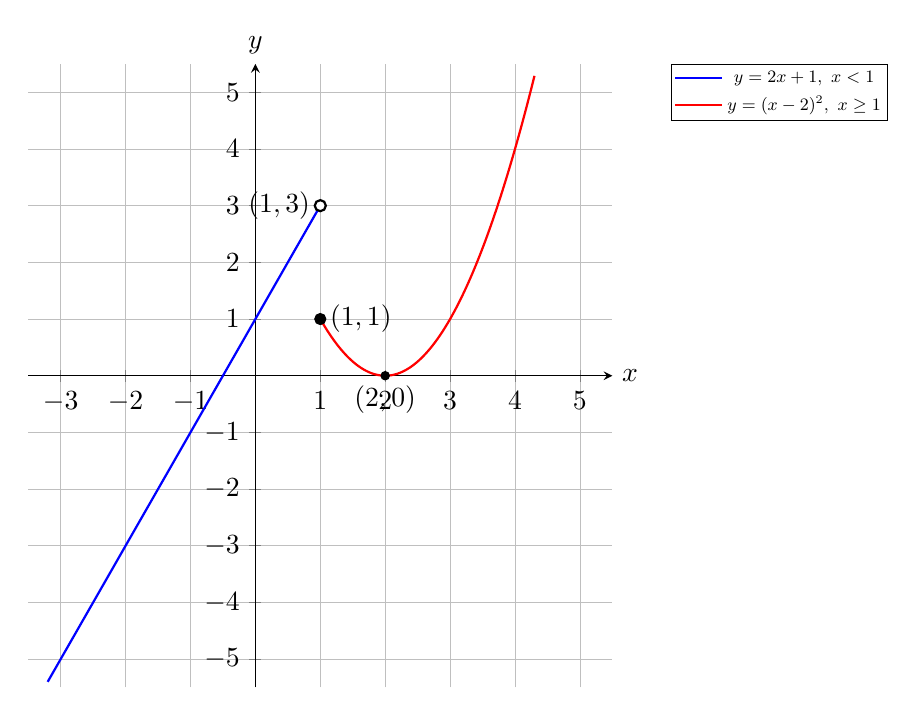
\begin{tikzpicture}
                    \begin{axis}[
        axis lines = middle,
        xlabel = $x$,
        ylabel = {$y$},
        grid=both,
        grid style={line width=.1pt, draw=gray!10},
        major grid style={line width=.2pt,draw=gray!50},
        x label style={anchor=west}, % label x ke kanan
        y label style={anchor=south}, % label y ke atas
        samples=200,
        legend style={
                at={(1.1,1)},
                anchor=north west,
                font=\small,         % mengecilkan ukuran font
                row sep=1pt,         % jarak antar baris legend
                inner sep=1pt,       % margin dalam kotak legend
                nodes={scale=0.7}    % skalakan isi legend
            },
        xtick={-3,-2,...,5},
        ytick={-5,-4,...,5},
        xmin=-3.5, xmax=5.5,
        ymin=-5.5, ymax=5.5,
        width=9cm,
        height=9.5cm
    ]
\addplot[domain=-3.2:1, color=blue, thick, samples=2] {2*x+1};
\addlegendentry{$y=2x+1,\ x<1$}
\addplot[domain=1:4.3, color=red, thick] {(x-2)^2};
\addlegendentry{$y=(x-2)^2,\ x\geq 1$}
\draw[fill=white, thick] (1,3) circle (2pt) node[left] {$(1,3)$};
\draw[fill=black] (1,1) circle (2pt) node[right] {$(1,1)$};
\draw[fill=black] (2,0) circle (1.5pt) node[below] {$(2,0)$};
\end{axis}
                \end{tikzpicture}
            \end{center}
        \end{enumerate}
    }
    \end{jawab}

    \item Diberikan fungsi $f(x)=\sqrt{4x-x^2},\ 0\leq x\leq 2$.
    \begin{enumerate}
        \item Tentukan $f^{-1}(x)$ beserta domainnya.
        \item Gambarkan grafik $f(x)$ dan $f^{-1}(x)$ dalam satu bidang koordinat.
    \end{enumerate}
    \begin{jawab}[melengkapkan kuadrat, setengah lingkaran, fungsi invers, sketsa grafik fungsi invers]{
        \begin{enumerate}
            \item Dengan melengkapkan kuadrat, diperoleh $4x-x^2 = 4-(x^2-4x+4) = \colorlet{oldcolor}{.}
        \color{blue}
        \setlength{\fboxrule}{1pt} \boxed{\color{oldcolor}4-(x-2)^2}\color{oldcolor}$, sehingga $f(x)=\sqrt{4-(x-2)^2}$. Grafik $f$ adalah bagian dari setengah lingkaran atas $(x-2)^2+y^2=4$ dengan pusat $(2,0)$ dan jari-jari $2$. Pada $0\leq x\leq 2$, fungsi $f$ naik dari $f(0)=0$ sampai $f(2)=2$, sehingga $f$ satu-satu dan $R(f)=[0,2]$.\\
            Misalkan $y=f(x)$ dengan $0\leq x\leq 2$, kemudian selesaikan sehingga terbentuk $x$ dalam fungsi $y$. Diperoleh
            \begin{align*}
                y &= \sqrt{4-(x-2)^2}\\
                y^2 &= 4-(x-2)^2\\
                (x-2)^2 &= 4-y^2\\
                x-2 &= -\sqrt{4-y^2} \quad (\text{karena } x\leq 2, \text{ yaitu } x-2\leq 0)\\
                x &= 2-\sqrt{4-y^2}.
            \end{align*}
            Dari sini didapatkan $x = f^{-1}(y) = 2-\sqrt{4-y^2}$. Dengan mengganti $y$ dengan $x$, dan mengingat bahwa domain dari fungsi invers adalah range dari fungsi asli, diperoleh
            \begin{align*}
                \colorlet{oldcolor}{.}
        \color{red}
        \setlength{\fboxrule}{1pt} \boxed{\color{oldcolor}f^{-1}(x) = 2-\sqrt{4-x^2},\quad D(f^{-1})=R(f)=[0,2]}\color{oldcolor}.
            \end{align*}
            \item Grafik $f$ adalah seperempat lingkaran berpusat di $(2,0)$ dari titik $(0,0)$ ke $(2,2)$. Grafik $f^{-1}$ merupakan pencerminan grafik $f$ terhadap garis $y=x$, yaitu seperempat lingkaran $x^2+(y-2)^2=4$ yang berpusat di $(0,2)$, juga dari titik $(0,0)$ ke $(2,2)$. Sketsa grafiknya adalah sebagai berikut.
            \begin{center}
                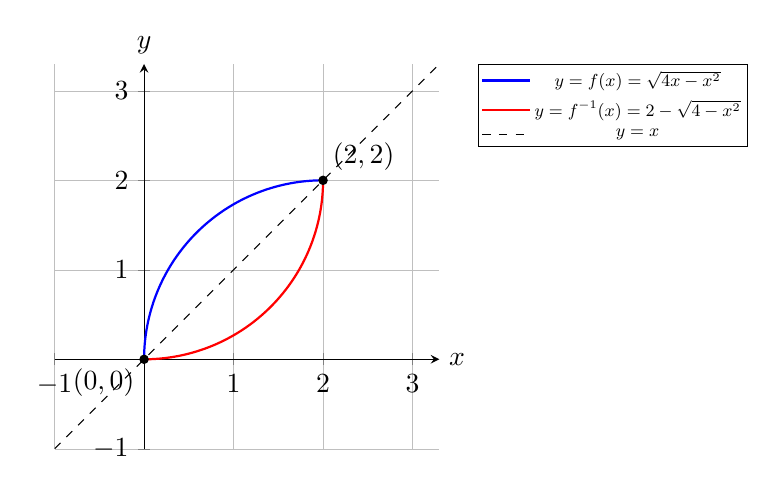
\begin{tikzpicture}
                    \begin{axis}[
        axis lines = middle,
        xlabel = $x$,
        ylabel = {$y$},
        grid=both,
        grid style={line width=.1pt, draw=gray!10},
        major grid style={line width=.2pt,draw=gray!50},
        x label style={anchor=west}, % label x ke kanan
        y label style={anchor=south}, % label y ke atas
        samples=200,
        legend style={
                at={(1.1,1)},
                anchor=north west,
                font=\small,         % mengecilkan ukuran font
                row sep=1pt,         % jarak antar baris legend
                inner sep=1pt,       % margin dalam kotak legend
                nodes={scale=0.7}    % skalakan isi legend
            },
        xtick={-1,0,...,3},
        ytick={-1,0,...,3},
        xmin=-1, xmax=3.3,
        ymin=-1, ymax=3.3,
        axis equal image,
        width=7.5cm
    ]
\addplot[domain=90:180, color=blue, thick] ({2+2*cos(x)}, {2*sin(x)});
\addlegendentry{$y=f(x)=\sqrt{4x-x^2}$}
\addplot[domain=90:180, color=red, thick] ({2*sin(x)}, {2+2*cos(x)});
\addlegendentry{$y=f^{-1}(x)=2-\sqrt{4-x^2}$}
\addplot[domain=-1:3.3, color=black, dashed, samples=2] {x};
\addlegendentry{$y=x$}
\draw[fill=black] (0,0) circle (1.5pt) node[below left] {$(0,0)$};
\draw[fill=black] (2,2) circle (1.5pt) node[above right] {$(2,2)$};
\end{axis}
                \end{tikzpicture}
            \end{center}
        \end{enumerate}
    }
    \end{jawab}

    \item Diberikan $f(x)=\dfrac{x^3+8}{x+2}$.
    \begin{enumerate}
        \item Tentukan $\displaystyle\lim_{x\to -2}f(x)$.
        \item Buatlah sketsa grafik $y=f(x)$.
    \end{enumerate}
    \begin{jawab}[limit fungsi, faktorisasi, sketsa grafik]{
        \begin{enumerate}
            \item Diperhatikan bahwa jika kita substitusi $x=-2$ ke dalam $f(x)$, maka diperoleh bentuk tak tentu $\frac{0}{0}$. Oleh karena itu, kita faktorkan pembilangnya dengan rumus $a^3+b^3=(a+b)(a^2-ab+b^2)$:
            \begin{align*}
                \colorlet{oldcolor}{.}
        \color{blue}
        \setlength{\fboxrule}{1pt} \boxed{\color{oldcolor}x^3+8 = (x+2)(x^2-2x+4)}\color{oldcolor}.
            \end{align*}
            Dengan demikian, fungsi dapat disederhanakan menjadi
            \begin{align*}
                f(x) = \frac{x^3+8}{x+2} = \frac{(x+2)(x^2-2x+4)}{x+2} = x^2-2x+4, \quad x\neq -2.
            \end{align*}
            Sehingga limitnya adalah
            \begin{align*}
                \lim_{x\to -2}f(x) = \lim_{x\to -2}(x^2-2x+4)= (-2)^2 - 2(-2) + 4= 12.
            \end{align*}
            Jadi $\colorlet{oldcolor}{.}
        \color{red}
        \setlength{\fboxrule}{1pt} \boxed{\color{oldcolor}\lim_{x\to -2}f(x) = 12}\color{oldcolor}$.
            \item Dari (a), grafik $y=f(x)$ sama dengan grafik parabola $y=x^2-2x+4=(x-1)^2+3$ yang terbuka ke atas dengan titik puncak $(1,3)$, tetapi titik $(-2,12)$ tidak termasuk dalam grafik (berlubang) karena $f(-2)$ tidak terdefinisi. Sebagai bantuan, grafik memotong sumbu-$y$ di titik $(0,4)$. Sketsa grafik dari $y=f(x)$ adalah sebagai berikut:
            \begin{center}
                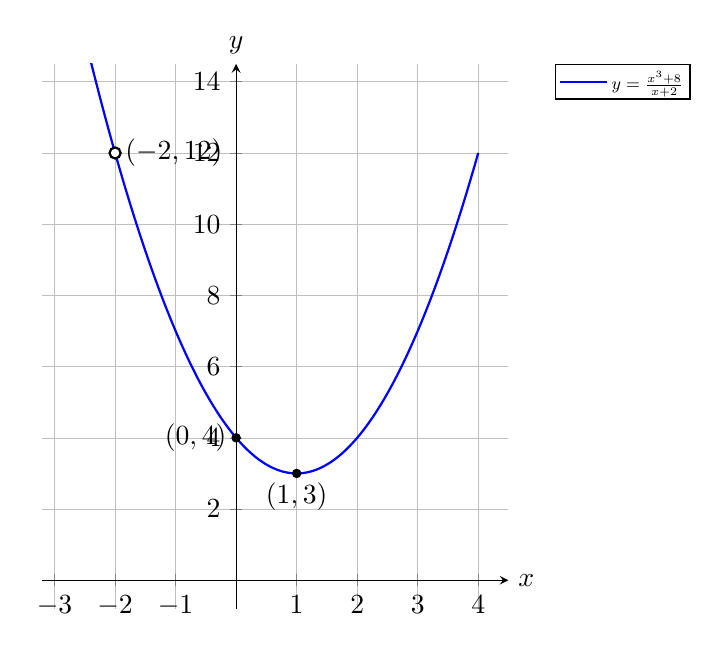
\begin{tikzpicture}
                    \begin{axis}[
        axis lines = middle,
        xlabel = $x$,
        ylabel = {$y$},
        grid=both,
        grid style={line width=.1pt, draw=gray!10},
        major grid style={line width=.2pt,draw=gray!50},
        x label style={anchor=west}, % label x ke kanan
        y label style={anchor=south}, % label y ke atas
        samples=200,
        legend style={
                at={(1.1,1)},
                anchor=north west,
                font=\small,         % mengecilkan ukuran font
                row sep=1pt,         % jarak antar baris legend
                inner sep=1pt,       % margin dalam kotak legend
                nodes={scale=0.7}    % skalakan isi legend
            },
        xtick={-3,-2,...,4},
        ytick={0,2,...,14},
        xmin=-3.2, xmax=4.5,
        ymin=-0.8, ymax=14.5,
        width=7.5cm,
        height=8.5cm
    ]
\addplot[domain=-2.7:4, color=blue, thick] {x^2-2*x+4};
\addlegendentry{$y=\frac{x^3+8}{x+2}$}
\draw[fill=white, thick] (-2,12) circle (2pt) node[right] {$(-2,12)$};
\draw[fill=black] (1,3) circle (1.5pt) node[below] {$(1,3)$};
\draw[fill=black] (0,4) circle (1.5pt) node[left] {$(0,4)$};
\end{axis}
                \end{tikzpicture}
            \end{center}
        \end{enumerate}
    }
    \end{jawab}

    \item Diketahui garis singgung pada kurva $x^2-xy+y^2=12$ di titik $(a,b)$ sejajar dengan sumbu-$x$. Tentukan semua titik $(a,b)$ dan persamaan garis singgungnya.
    \begin{jawab}[turunan implisit, garis singgung mendatar, persamaan garis singgung]{~\\
        Garis yang sejajar dengan sumbu-$x$ memiliki gradien nol, sehingga di titik $(a,b)$ haruslah $\colorlet{oldcolor}{.}
        \color{blue}
        \setlength{\fboxrule}{1pt} \boxed{\color{oldcolor}\frac{dy}{dx}=0}\color{oldcolor}$. Kita turunkan kedua ruas persamaan kurva terhadap $x$, dengan aturan perkalian $\frac{d}{dx}(xy)=y+x\frac{dy}{dx}$ dan aturan rantai $\frac{d}{dx}(y^2)=2y\frac{dy}{dx}$:
        \begin{align*}
            2x - \left(y + x\frac{dy}{dx}\right) + 2y\frac{dy}{dx} &= 0\\
            (2y - x)\frac{dy}{dx} &= y - 2x\\
            \frac{dy}{dx} &= \colorlet{oldcolor}{.}
        \color{blue}
        \setlength{\fboxrule}{1pt} \boxed{\color{oldcolor}\frac{y-2x}{2y-x}}\color{oldcolor}.
        \end{align*}
        Agar $\frac{dy}{dx}=0$ di titik $(a,b)$, haruslah pembilangnya nol (dengan penyebut tidak nol), yaitu $b-2a=0$ atau $\colorlet{oldcolor}{.}
        \color{blue}
        \setlength{\fboxrule}{1pt} \boxed{\color{oldcolor}b=2a}\color{oldcolor}$. Karena titik $(a,b)$ terletak pada kurva, substitusi $b=2a$ ke persamaan kurva:
        \begin{align*}
            a^2 - a(2a) + (2a)^2 &= 12\\
            a^2 - 2a^2 + 4a^2 &= 12\\
            3a^2 &= 12\\
            a^2 &= 4 \implies a=\pm 2.
        \end{align*}
        Untuk $a=2$ diperoleh $b=4$, dan untuk $a=-2$ diperoleh $b=-4$. Dicek penyebutnya, yaitu $2(4)-2=6\neq 0$ dan $2(-4)-(-2)=-6\neq 0$. Jadi titik-titik yang dimaksud adalah $\colorlet{oldcolor}{.}
        \color{red}
        \setlength{\fboxrule}{1pt} \boxed{\color{oldcolor}(2,4) \text{ dan } (-2,-4)}\color{oldcolor}$.\\
        Garis singgung yang sejajar sumbu-$x$ berbentuk $y=b$, sehingga persamaan garis singgungnya adalah
        \begin{align*}
            \colorlet{oldcolor}{.}
        \color{red}
        \setlength{\fboxrule}{1pt} \boxed{\color{oldcolor}y=4 \text{ (di titik } (2,4)) \quad\text{dan}\quad y=-4 \text{ (di titik } (-2,-4))}\color{oldcolor}.
        \end{align*}
    }
    \end{jawab}
\end{enumerate}

\newpage

%%%%%%%%%%%%%%%%%%%%%%%%%%%%%%%%%%%%%%%%%%%%%%%%%%%%%%%%%%%%%%%%%%%%%%%%%%%%%%
% Kal-iup-2
\kopsoaliup{Kal-iup-2}{62, 69}{Mechanical, Industrial, Materials \& Metallurgical Engineering}{Monday, Wednesday; 15.30-17.10}{4}
\begin{enumerate}
    \item Find the solution of the following inequality
    \begin{align*}
        \frac{x^2+x-6}{x^2-3x-4}\geq 0.
    \end{align*}
    \begin{jawab}[pertidaksamaan rasional, faktorisasi, garis bilangan, notasi interval]{~\\
    Karena ruas kanan pertidaksamaan sudah bernilai nol, maka kita bisa langsung memfaktorkan pembilang dan penyebut di ruas kiri. Diperoleh
    \begin{align*}
        \frac{x^2+x-6}{x^2-3x-4} = \frac{(x+3)(x-2)}{(x-4)(x+1)} \geq 0.
    \end{align*}
    Selanjutnya, kita tentukan pembuat nol dari faktor-faktor tersebut, yaitu
    \begin{align*}
        x+3 = 0 \quad &\vee\quad x-2 = 0 \quad \vee\quad x-4 = 0 \quad \vee\quad x+1 = 0\\
        \colorlet{oldcolor}{.}
        \color{blue}
        \setlength{\fboxrule}{1pt} \boxed{\color{oldcolor}x=-3}\color{oldcolor} \quad &\vee\quad \colorlet{oldcolor}{.}
        \color{blue}
        \setlength{\fboxrule}{1pt} \boxed{\color{oldcolor}x=2}\color{oldcolor} \quad \vee\quad \colorlet{oldcolor}{.}
        \color{blue}
        \setlength{\fboxrule}{1pt} \boxed{\color{oldcolor}x=4}\color{oldcolor} \quad \vee\quad \colorlet{oldcolor}{.}
        \color{blue}
        \setlength{\fboxrule}{1pt} \boxed{\color{oldcolor}x=-1}\color{oldcolor}
    \end{align*}
    Selanjutnya, kita buat garis bilangan dan lakukan uji titik pada ekspresi \(\frac{(x+3)(x-2)}{(x-4)(x+1)}\) sebagai berikut
    \begin{itemize}
        \item Untuk \(x < -3\), misalkan \(x = -4\):
        \[
        \frac{(-4+3)(-4-2)}{(-4-4)(-4+1)} = \frac{(-1)(-6)}{(-8)(-3)} = \frac{6}{24} > 0
        \]
        \item Untuk \(-3 < x < -1\), misalkan \(x = -2\):
        \[
        \frac{(-2+3)(-2-2)}{(-2-4)(-2+1)} = \frac{(1)(-4)}{(-6)(-1)} = \frac{-4}{6} < 0
        \]
        \item Untuk \(-1 < x < 2\), misalkan \(x = 0\):
        \[
        \frac{(0+3)(0-2)}{(0-4)(0+1)} = \frac{(3)(-2)}{(-4)(1)} = \frac{6}{4} > 0
        \]
        \item Untuk \(2 < x < 4\), misalkan \(x = 3\):
        \[
        \frac{(3+3)(3-2)}{(3-4)(3+1)} = \frac{(6)(1)}{(-1)(4)} = \frac{-6}{4} < 0
        \]
        \item Untuk \(x > 4\), misalkan \(x = 5\):
        \[
        \frac{(5+3)(5-2)}{(5-4)(5+1)} = \frac{(8)(3)}{(1)(6)} = 4 > 0
        \]
    \end{itemize}
    \begin{center}
        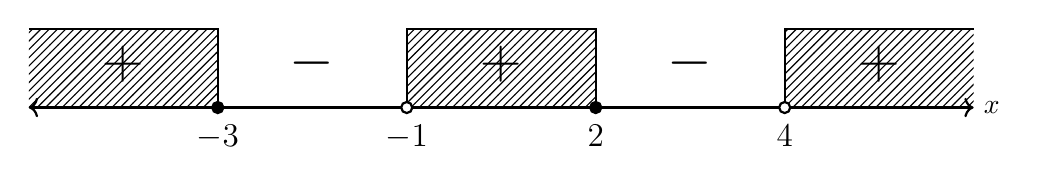
\begin{tikzpicture}
    \draw[thick,<->] (-6,0) -- (6,0) node[right] {$x$};
    \fill[pattern=north east lines] (-6,0) rectangle (-3.6,1);
    \fill[pattern=north east lines] (-1.2,0) rectangle (1.2,1);
    \fill[pattern=north east lines] (3.6,0) rectangle (6,1);
    \draw[thick] (-6,1) -- (-3.6,1) -- (-3.6,0);
    \draw[thick] (-1.2,0) -- (-1.2,1) -- (1.2,1) -- (1.2,0);
    \draw[thick] (3.6,0) -- (3.6,1) -- (6,1);
    \draw (-3.6,-0.1) node[below] {\large{$-3$}};
    \draw (-1.2,-0.1) node[below] {\large{$-1$}};
    \draw (1.2,-0.1) node[below] {\large{$2$}};
    \draw (3.6,-0.1) node[below] {\large{$4$}};
    \draw (-4.8,0.2) node[above] {\huge{$+$}};
    \draw (-2.4,0.2) node[above] {\huge{$-$}};
    \draw (0,0.2) node[above] {\huge{$+$}};
    \draw (2.4,0.2) node[above] {\huge{$-$}};
    \draw (4.8,0.2) node[above] {\huge{$+$}};
    \draw[fill=black, thick] (-3.6,0) circle (2pt);
    \draw[fill=white, thick] (-1.2,0) circle (2pt);
    \draw[fill=black, thick] (1.2,0) circle (2pt);
    \draw[fill=white, thick] (3.6,0) circle (2pt);
        \end{tikzpicture}
    \end{center}
    Karena yang diminta adalah nilai yang lebih dari atau sama dengan nol, diambil interval yang bertanda positif beserta pembuat nol dari pembilang ($x=-3$ dan $x=2$). Pembuat nol dari penyebut ($x=-1$ dan $x=4$) tidak diikutkan karena membuat ekspresi tidak terdefinisi. Jadi solusi dari pertidaksamaan tersebut adalah \(x \leq -3\) atau \(-1 < x \leq 2\) atau \(x > 4\). Dalam notasi interval, solusi tersebut dapat ditulis sebagai $\colorlet{oldcolor}{.}
        \color{red}
        \setlength{\fboxrule}{1pt} \boxed{\color{oldcolor}(-\infty, -3] \cup (-1, 2] \cup (4, \infty)}\color{oldcolor}$.
    }
    \end{jawab}

    \item \begin{enumerate}
        \item Find the gradient of the line $\ell$ which goes through $(0,0)$ and $(3,-4)$.
        \item If line $\ell$ is perpendicular with the line that tangent with a circle centered at $(0,0)$ and radius $5$, at $(3,-4)$, then find the aforementioned tangent line equation and sketch the graph.
    \end{enumerate}
    \begin{jawab}[kemiringan garis, garis tegak lurus, garis singgung lingkaran]{
        \begin{enumerate}
            \item Kemiringan garis yang melalui dua titik $(x_1,y_1)$ dan $(x_2,y_2)$ adalah
            \begin{align*}
                m = \frac{y_2 - y_1}{x_2 - x_1}.
            \end{align*}
            Dengan substitusi $(x_1,y_1)=(0,0)$ dan $(x_2,y_2)=(3,-4)$, diperoleh
            \begin{align*}
                m_\ell = \frac{-4 - 0}{3 - 0} = -\frac{4}{3}.
            \end{align*}
            Jadi kemiringan garis $\ell$ adalah $\colorlet{oldcolor}{.}
        \color{red}
        \setlength{\fboxrule}{1pt} \boxed{\color{oldcolor}m_\ell = -\frac{4}{3}}\color{oldcolor}$.
            \item Persamaan lingkaran yang berpusat di $(0,0)$ dan berjari-jari $5$ adalah $x^2 + y^2 = 25$. Diperhatikan bahwa titik $(3,-4)$ terletak pada lingkaran, karena $3^2 + (-4)^2 = 9 + 16 = 25$. \\
            Ingat kembali bahwa dua garis dengan gradien $m_1$ dan $m_2$ saling tegak lurus jika $\colorlet{oldcolor}{.}
        \color{blue}
        \setlength{\fboxrule}{1pt} \boxed{\color{oldcolor}m_1\cdot m_2=-1}\color{oldcolor}$. Karena garis singgung tegak lurus dengan garis $\ell$, maka gradien garis singgung $m_s$ memenuhi
            \begin{align*}
                m_\ell \cdot m_s = -1 \implies -\frac{4}{3}\cdot m_s = -1 \implies \colorlet{oldcolor}{.}
        \color{blue}
        \setlength{\fboxrule}{1pt} \boxed{\color{oldcolor}m_s = \frac{3}{4}}\color{oldcolor}.
            \end{align*}
            Garis singgung melalui titik $(3,-4)$ dengan gradien $\frac{3}{4}$, sehingga dengan rumus $y - y_1 = m(x - x_1)$ diperoleh
            \begin{align*}
                y - (-4) &= \frac{3}{4}(x - 3)\\
                y + 4 &= \frac{3}{4}x - \frac{9}{4}\\
                y &= \frac{3}{4}x - \frac{25}{4}.
            \end{align*}
            Jadi persamaan garis singgung lingkaran tersebut adalah $\colorlet{oldcolor}{.}
        \color{red}
        \setlength{\fboxrule}{1pt} \boxed{\color{oldcolor}y = \frac{3}{4}x - \frac{25}{4}}\color{oldcolor}$ atau $3x-4y=25$. Sketsa grafiknya adalah sebagai berikut:
            \begin{center}
                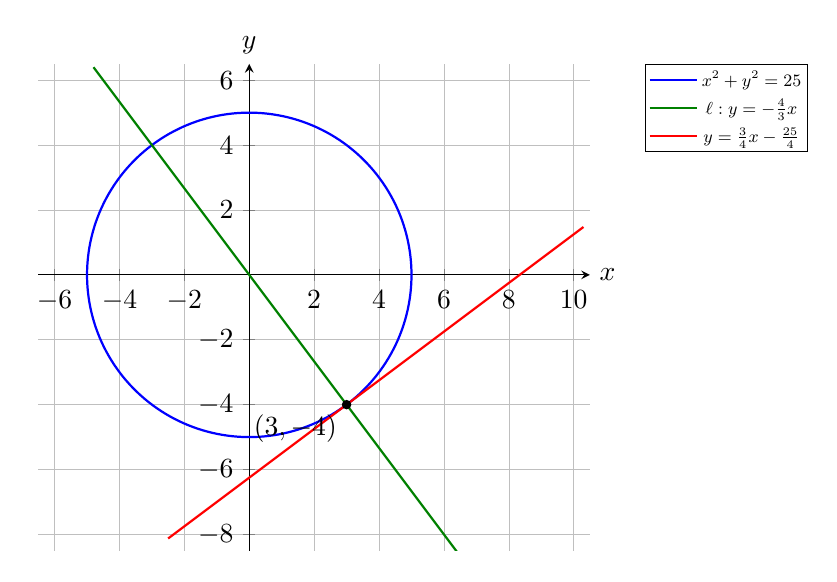
\begin{tikzpicture}
                    \begin{axis}[
        axis lines = middle,
        xlabel = $x$,
        ylabel = {$y$},
        grid=both,
        grid style={line width=.1pt, draw=gray!10},
        major grid style={line width=.2pt,draw=gray!50},
        x label style={anchor=west}, % label x ke kanan
        y label style={anchor=south}, % label y ke atas
        samples=200,
        legend style={
                at={(1.1,1)},
                anchor=north west,
                font=\small,         % mengecilkan ukuran font
                row sep=1pt,         % jarak antar baris legend
                inner sep=1pt,       % margin dalam kotak legend
                nodes={scale=0.7}    % skalakan isi legend
            },
        xtick={-6,-4,...,10},
        ytick={-8,-6,...,6},
        xmin=-6.5, xmax=10.5,
        ymin=-8.5, ymax=6.5,
        axis equal image,
        width=9cm
    ]
\addplot[domain=0:360, color=blue, thick] ({5*cos(x)}, {5*sin(x)});
\addlegendentry{$x^2+y^2=25$}
\addplot[domain=-4.8:6.4, color=green!50!black, thick, samples=2] {-4*x/3};
\addlegendentry{$\ell: y=-\frac{4}{3}x$}
\addplot[domain=-2.5:10.3, color=red, thick, samples=2] {3*x/4-25/4};
\addlegendentry{$y=\frac{3}{4}x-\frac{25}{4}$}
\draw[fill=black] (3,-4) circle (1.5pt) node[below left] {$(3,-4)$};
\end{axis}
                \end{tikzpicture}
            \end{center}
        \end{enumerate}
    }
    \end{jawab}

    \item Write the derivative formula of $fg$ that is $\dfrac{d}{dx}(f(x)g(x))$\\
    Then, find the derivative of $fg$, given that $f(x)=2x^3-x$ and $g(x)=4-x^2$.
    \begin{jawab}[turunan, aturan perkalian]{~\\
        Ingat kembali aturan turunan untuk perkalian fungsi, yaitu
        \[
        \colorlet{oldcolor}{.}
        \color{red}
        \setlength{\fboxrule}{1pt} \boxed{\color{oldcolor}\frac{d}{dx}\left(f(x)g(x)\right) = f'(x)g(x) + f(x)g'(x)}\color{oldcolor}.
        \]
        Selanjutnya, kita hitung turunan dari \(f(x)\) dan \(g(x)\):
        \begin{align*}
            \colorlet{oldcolor}{.}
        \color{blue}
        \setlength{\fboxrule}{1pt} \boxed{\color{oldcolor}f'(x) = \frac{d}{dx}(2x^3 - x) = 6x^2 - 1}\color{oldcolor}\\
            \colorlet{oldcolor}{.}
        \color{blue}
        \setlength{\fboxrule}{1pt} \boxed{\color{oldcolor}g'(x) = \frac{d}{dx}(4 - x^2) = -2x}\color{oldcolor}
        \end{align*}
        Dengan demikian, turunan dari \(fg\) adalah
        \begin{align*}
            \frac{d}{dx}\left(f(x)g(x)\right) &= (6x^2 - 1)(4 - x^2) + (2x^3 - x)(-2x)\\
            &= (24x^2 - 6x^4 - 4 + x^2) + (-4x^4 + 2x^2)\\
            &= \colorlet{oldcolor}{.}
        \color{red}
        \setlength{\fboxrule}{1pt} \boxed{\color{oldcolor}-10x^4 + 27x^2 - 4}\color{oldcolor}.
        \end{align*}
    }
    \end{jawab}

    \item Calculate $\displaystyle\lim_{x\to 2}\frac{\sqrt{4x+1}-3}{x-2}$.
    \begin{jawab}[limit fungsi, bentuk tak tentu, perkalian sekawan]{~\\
        Diperhatikan bahwa jika kita substitusi $x=2$ secara langsung, diperoleh $\frac{\sqrt{9}-3}{0}=\frac{0}{0}$ yang merupakan bentuk tak tentu. Untuk menyelesaikan limit tersebut, kita kalikan dengan bentuk konjugat (sekawan) dari pembilangnya, sehingga diperoleh
        \begin{align*}
            \lim_{x\to 2} \frac{\sqrt{4x+1}-3}{x-2} &= \lim_{x\to 2} \frac{\sqrt{4x+1}-3}{x-2}\cdot\frac{\sqrt{4x+1}+3}{\sqrt{4x+1}+3}\\
            &= \lim_{x\to 2} \frac{4x+1-9}{(x-2)(\sqrt{4x+1}+3)}\\
            &= \lim_{x\to 2} \frac{4(x-2)}{(x-2)(\sqrt{4x+1}+3)}\\
            &= \lim_{x\to 2} \frac{4}{\sqrt{4x+1}+3}\\
            &= \frac{4}{\sqrt{9}+3}\\
            &= \colorlet{oldcolor}{.}
        \color{red}
        \setlength{\fboxrule}{1pt} \boxed{\color{oldcolor}\frac{2}{3}}\color{oldcolor}.
        \end{align*}
    }
    \end{jawab}

    \item Given a function $f(x)=\dfrac{1}{x+2}$ and $g(x)=x^2$.
    \begin{enumerate}
        \item Find $(f\circ g)(x)$.
        \item Given $(p\circ g)(x)=x^2+5$, then find $p(x)$.
    \end{enumerate}
    \begin{jawab}[fungsi komposisi]{
        \begin{enumerate}
            \item Diperhatikan bahwa
            \begin{align*}
                (f\circ g)(x) = f(g(x)) = f(x^2) = \colorlet{oldcolor}{.}
        \color{red}
        \setlength{\fboxrule}{1pt} \boxed{\color{oldcolor}\frac{1}{x^2+2}}\color{oldcolor},
            \end{align*}
            dengan domain $\mathbb{R}$, karena $x^2+2\geq 2>0$ untuk setiap $x$.
            \item Diperhatikan bahwa $(p\circ g)(x) = p(g(x)) = p(x^2) = x^2+5$. Misalkan $\colorlet{oldcolor}{.}
        \color{blue}
        \setlength{\fboxrule}{1pt} \boxed{\color{oldcolor}u = x^2}\color{oldcolor}$, maka diperoleh
            \begin{align*}
                p(u) = u + 5.
            \end{align*}
            Dengan mengganti $u$ dengan $x$, didapatkan $\colorlet{oldcolor}{.}
        \color{red}
        \setlength{\fboxrule}{1pt} \boxed{\color{oldcolor}p(x) = x + 5}\color{oldcolor}$.\\
            Sebagai pengecekan, $(p\circ g)(x) = p(x^2) = x^2 + 5$, sesuai dengan yang diketahui.
        \end{enumerate}
    }
    \end{jawab}
\end{enumerate}

\newpage

%%%%%%%%%%%%%%%%%%%%%%%%%%%%%%%%%%%%%%%%%%%%%%%%%%%%%%%%%%%%%%%%%%%%%%%%%%%%%%
% Kal-3
\kopsoal{Kal-3}{13-16}{Kimia, Saik, Telkom}{Selasa, Kamis; 07.00-09.30}{6}
\begin{enumerate}
    \item Dapatkan penyelesaian dari pertidaksamaan
    \begin{align*}
        1\leq x^2-3\leq 13.
    \end{align*}
    \begin{jawab}[pertidaksamaan kuadrat, pertidaksamaan ganda, garis bilangan, notasi interval]{~\\
        Dengan menambahkan $3$ pada setiap ruas, pertidaksamaan ganda tersebut menjadi
        \begin{align*}
            4\leq x^2\leq 16,
        \end{align*}
        yang dapat dipecah menjadi dua pertidaksamaan yang harus dipenuhi sekaligus, yaitu $\colorlet{oldcolor}{.}
        \color{blue}
        \setlength{\fboxrule}{1pt} \boxed{\color{oldcolor}x^2\geq 4}\color{oldcolor}$ dan $\colorlet{oldcolor}{.}
        \color{blue}
        \setlength{\fboxrule}{1pt} \boxed{\color{oldcolor}x^2\leq 16}\color{oldcolor}$.
        \begin{itemize}
            \item Untuk $x^2\geq 4$, diperoleh $x^2-4=(x-2)(x+2)\geq 0$. Pembuat nolnya adalah $x=-2$ dan $x=2$. Dengan uji titik (misalnya $x=-3$, $x=0$, dan $x=3$), diperoleh tanda $+$, $-$, $+$, sehingga penyelesaiannya adalah $x\leq -2$ atau $x\geq 2$.
            \item Untuk $x^2\leq 16$, diperoleh $x^2-16=(x-4)(x+4)\leq 0$. Pembuat nolnya adalah $x=-4$ dan $x=4$. Dengan uji titik (misalnya $x=-5$, $x=0$, dan $x=5$), diperoleh tanda $+$, $-$, $+$, sehingga penyelesaiannya adalah $-4\leq x\leq 4$.
        \end{itemize}
        Penyelesaian dari pertidaksamaan ganda adalah irisan dari kedua penyelesaian tersebut, yang dapat digambarkan pada garis bilangan sebagai berikut
        \begin{center}
            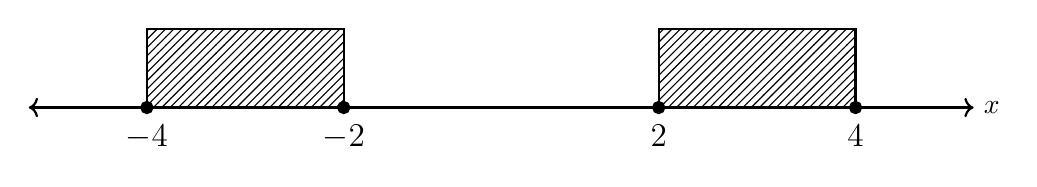
\begin{tikzpicture}
    \draw[thick,<->] (-6,0) -- (6,0) node[right] {$x$};
    \fill[pattern=north east lines] (-4.5,0) rectangle (-2,1);
    \fill[pattern=north east lines] (2,0) rectangle (4.5,1);
    \draw[thick] (-4.5,0) -- (-4.5,1) -- (-2,1) -- (-2,0);
    \draw[thick] (2,0) -- (2,1) -- (4.5,1) -- (4.5,0);
    \draw (-4.5,-0.1) node[below] {\large{$-4$}};
    \draw (-2,-0.1) node[below] {\large{$-2$}};
    \draw (2,-0.1) node[below] {\large{$2$}};
    \draw (4.5,-0.1) node[below] {\large{$4$}};
    \draw[fill=black, thick] (-4.5,0) circle (2pt);
    \draw[fill=black, thick] (-2,0) circle (2pt);
    \draw[fill=black, thick] (2,0) circle (2pt);
    \draw[fill=black, thick] (4.5,0) circle (2pt);
            \end{tikzpicture}
        \end{center}
        Sebagai pengecekan, untuk $x=3$ diperoleh $x^2-3=6$ dan berlaku $1\leq 6\leq 13$, sedangkan untuk $x=0$ diperoleh $x^2-3=-3<1$. Jadi penyelesaiannya adalah $-4\leq x\leq -2$ atau $2\leq x\leq 4$, atau dalam notasi interval $\colorlet{oldcolor}{.}
        \color{red}
        \setlength{\fboxrule}{1pt} \boxed{\color{oldcolor}[-4,-2]\cup[2,4]}\color{oldcolor}$.
    }
    \end{jawab}

    \item Tentukan domain dari fungsi $(f\circ g)(x)$ jika diketahui fungsi $g(x)=3x-1$ dengan $0\leq x<2$ dan fungsi $f$ terdefinisi pada interval $1\leq x<4$.
    \begin{jawab}[domain fungsi komposisi, pertidaksamaan linear]{~\\
        Dari soal diketahui bahwa $\colorlet{oldcolor}{.}
        \color{blue}
        \setlength{\fboxrule}{1pt} \boxed{\color{oldcolor}D(g)=[0,2)}\color{oldcolor}$ dan $\colorlet{oldcolor}{.}
        \color{blue}
        \setlength{\fboxrule}{1pt} \boxed{\color{oldcolor}D(f)=[1,4)}\color{oldcolor}$. Domain dari fungsi komposisi $f\circ g$ adalah semua nilai $x$ pada domain $g$ sehingga nilai dari $g(x)$ berada pada domain $f$, yang dapat dirumuskan sebagai
        \begin{align*}
            \colorlet{oldcolor}{.}
        \color{blue}
        \setlength{\fboxrule}{1pt} \boxed{\color{oldcolor}D(f\circ g) = \{x \in D(g) : g(x) \in D(f)\} = \{x \in [0,2) : 1\leq 3x-1<4\}}\color{oldcolor}.
        \end{align*}
        Selanjutnya, diselesaikan pertidaksamaan ganda $1\leq 3x-1<4$:
        \begin{align*}
            1\leq 3x-1<4 \iff 2\leq 3x<5 \iff \frac{2}{3}\leq x<\frac{5}{3}.
        \end{align*}
        Irisan dari $\left[\frac{2}{3},\frac{5}{3}\right)$ dengan $D(g)=[0,2)$ adalah $\left[\frac{2}{3},\frac{5}{3}\right)$, karena $0<\frac{2}{3}$ dan $\frac{5}{3}<2$. Jadi
        \begin{align*}
            \colorlet{oldcolor}{.}
        \color{red}
        \setlength{\fboxrule}{1pt} \boxed{\color{oldcolor}D(f\circ g) = \left\{x\in\mathbb{R} : \frac{2}{3}\leq x<\frac{5}{3}\right\} = \left[\frac{2}{3},\frac{5}{3}\right)}\color{oldcolor}.
        \end{align*}
    }
    \end{jawab}

    \item Gunakan grafik dasar $x=y^2$ dan sifat pergeseran/translasi untuk menggambar parabola $x=y^2-4y+1$.
    \begin{jawab}[parabola, melengkapkan kuadrat, translasi grafik]{~\\
        Kurva dasar $x=y^2$ merupakan parabola yang terbuka ke kanan dengan titik puncak $(0,0)$. Selanjutnya, bentuk $x = y^2 - 4y + 1$ diubah dengan cara melengkapkan kuadrat, yaitu
        \begin{align*}
            x &= y^2 - 4y + 1\\
            &= (y^2 - 4y + 4) - 4 + 1\\
            &= \colorlet{oldcolor}{.}
        \color{blue}
        \setlength{\fboxrule}{1pt} \boxed{\color{oldcolor}(y-2)^2 - 3}\color{oldcolor}.
        \end{align*}
        Ingat kembali bahwa mengganti $y$ dengan $y-2$ berarti menggeser grafik sejauh $2$ satuan ke atas, dan menambahkan konstanta $-3$ pada $x$ berarti menggeser grafik sejauh $3$ satuan ke kiri. Dengan demikian, proses translasinya adalah sebagai berikut.
        \begin{enumerate}
            \item[(i)] Gambar kurva dasar $x=y^2$ dengan titik puncak $(0,0)$.
            \item[(ii)] Geser kurva $x=y^2$ sejauh $2$ satuan ke atas, sehingga diperoleh kurva $x=(y-2)^2$ dengan titik puncak $(0,2)$.
            \item[(iii)] Geser kurva $x=(y-2)^2$ sejauh $3$ satuan ke kiri, sehingga diperoleh kurva $x=(y-2)^2-3$ dengan titik puncak $\colorlet{oldcolor}{.}
        \color{blue}
        \setlength{\fboxrule}{1pt} \boxed{\color{oldcolor}(-3,2)}\color{oldcolor}$.
        \end{enumerate}
        Sebagai bantuan, titik potong kurva dengan sumbu-$x$ ($y=0$) adalah $x=1$, yaitu titik $(1,0)$, sedangkan titik potong dengan sumbu-$y$ ($x=0$) adalah $(y-2)^2=3$, yaitu $y=2\pm\sqrt{3}$. Sketsa grafiknya adalah sebagai berikut.
        \begin{center}
            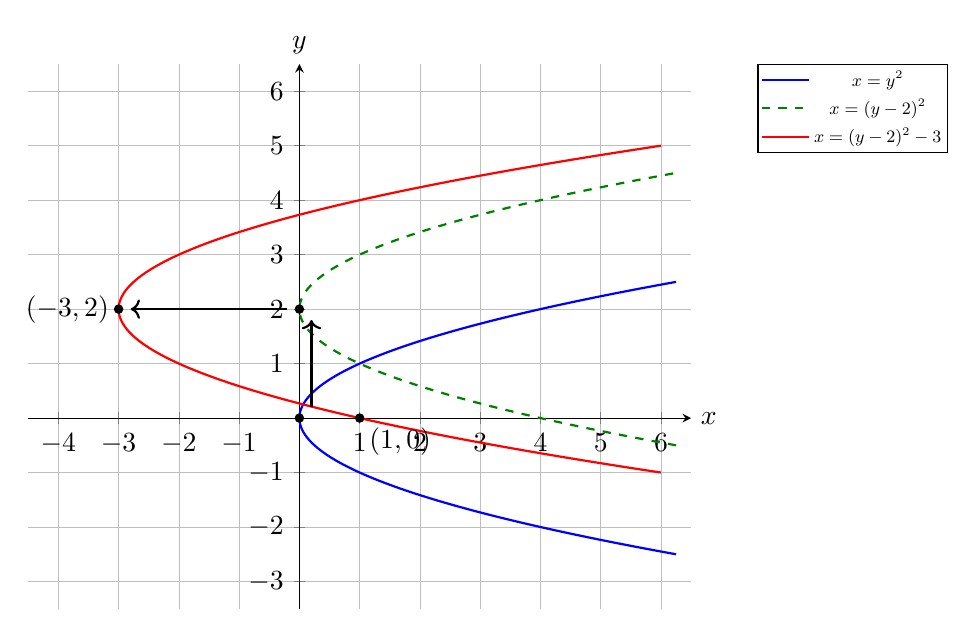
\begin{tikzpicture}
                \begin{axis}[
        axis lines = middle,
        xlabel = $x$,
        ylabel = {$y$},
        grid=both,
        grid style={line width=.1pt, draw=gray!10},
        major grid style={line width=.2pt,draw=gray!50},
        x label style={anchor=west}, % label x ke kanan
        y label style={anchor=south}, % label y ke atas
        samples=200,
        legend style={
                at={(1.1,1)},
                anchor=north west,
                font=\small,         % mengecilkan ukuran font
                row sep=1pt,         % jarak antar baris legend
                inner sep=1pt,       % margin dalam kotak legend
                nodes={scale=0.7}    % skalakan isi legend
            },
        xtick={-4,-3,...,6},
        ytick={-3,-2,...,6},
        xmin=-4.5, xmax=6.5,
        ymin=-3.5, ymax=6.5,
        width=10cm,
        height=8.5cm
    ]
\addplot[domain=-2.5:2.5, color=blue, thick] ({(x)*(x)},{x});
\addlegendentry{$x=y^2$}
\addplot[domain=-0.5:4.5, color=green!50!black, thick, dashed] ({(x-2)*(x-2)},{x});
\addlegendentry{$x=(y-2)^2$}
\addplot[domain=-1:5, color=red, thick] ({(x-2)*(x-2)-3},{x});
\addlegendentry{$x=(y-2)^2-3$}
\draw[fill=black] (0,0) circle (1.5pt);
\draw[fill=black] (0,2) circle (1.5pt);
\draw[fill=black] (-3,2) circle (1.5pt) node[left] {$(-3,2)$};
\draw[fill=black] (1,0) circle (1.5pt) node[below right] {$(1,0)$};
\draw[->, thick] (0.2,0.2) -- (0.2,1.8);
\draw[->, thick] (-0.2,2) -- (-2.8,2);
\end{axis}
            \end{tikzpicture}
        \end{center}
        Jadi kurva $x = y^2 - 4y + 1$ adalah
        \[\colorlet{oldcolor}{.}
        \color{red}
        \setlength{\fboxrule}{1pt} \boxed{\color{oldcolor}\text{parabola } x=y^2 \text{ yang digeser 2 satuan ke atas dan 3 satuan ke kiri}}\color{oldcolor}.\]
    }
    \end{jawab}

    \item Diberikan $f(x)=\begin{cases}
        k^2(x-1), & x\leq 2\\
        k(x+1), & x>2
    \end{cases}$.\\
    Tentukan semua nilai $k$ yang memenuhi agar $\displaystyle\lim_{x\to 2}f(x)$ ada.
    \begin{jawab}[limit sepihak, fungsi sepotong-sepotong, persamaan kuadrat]{~\\
        Ingat kembali bahwa $\displaystyle\lim_{x\to a}f(x)$ ada jika dan hanya jika limit kiri dan limit kanannya ada dan bernilai sama, yaitu $\colorlet{oldcolor}{.}
        \color{blue}
        \setlength{\fboxrule}{1pt} \boxed{\color{oldcolor}\lim_{x \to a^-} f(x) = \lim_{x \to a^+} f(x)}\color{oldcolor}$. Untuk $x\to 2^-$ (yaitu $x<2$) digunakan rumus $k^2(x-1)$, dan untuk $x\to 2^+$ (yaitu $x>2$) digunakan rumus $k(x+1)$. Diperoleh
        \begin{align*}
            \lim_{x\to 2^-} f(x) = \lim_{x\to 2^-} k^2(x-1) = k^2 \quad\text{dan}\quad \lim_{x\to 2^+} f(x) = \lim_{x\to 2^+} k(x+1) = 3k.
        \end{align*}
        Agar limitnya ada, haruslah
        \begin{align*}
            k^2 &= 3k\\
            k^2-3k &= 0\\
            k(k-3) &= 0,
        \end{align*}
        sehingga $k=0$ atau $k=3$. Jadi semua nilai $k$ yang memenuhi adalah $\colorlet{oldcolor}{.}
        \color{red}
        \setlength{\fboxrule}{1pt} \boxed{\color{oldcolor}k=0 \text{ atau } k=3}\color{oldcolor}$.\\
        Sebagai pengecekan, untuk $k=0$ kedua limit sepihak bernilai $0$, sedangkan untuk $k=3$ kedua limit sepihak bernilai $9$.
    }
    \end{jawab}

    \item Diketahui garis singgung pada kurva $x^2+xy+y^2=3$ di titik $(a,b)$ sejajar dengan garis $y=-x$. Tentukan semua titik $(a,b)$ dan persamaan garis singgungnya.
    \begin{jawab}[turunan implisit, garis sejajar, persamaan garis singgung]{~\\
        Garis $y=-x$ memiliki gradien $-1$. Karena garis singgung sejajar dengan garis tersebut, maka di titik $(a,b)$ haruslah $\colorlet{oldcolor}{.}
        \color{blue}
        \setlength{\fboxrule}{1pt} \boxed{\color{oldcolor}\frac{dy}{dx}=-1}\color{oldcolor}$. Kita turunkan kedua ruas persamaan kurva terhadap $x$, dengan aturan perkalian $\frac{d}{dx}(xy)=y+x\frac{dy}{dx}$ dan aturan rantai $\frac{d}{dx}(y^2)=2y\frac{dy}{dx}$:
        \begin{align*}
            2x + y + x\frac{dy}{dx} + 2y\frac{dy}{dx} &= 0\\
            (x + 2y)\frac{dy}{dx} &= -(2x + y)\\
            \frac{dy}{dx} &= \colorlet{oldcolor}{.}
        \color{blue}
        \setlength{\fboxrule}{1pt} \boxed{\color{oldcolor}-\frac{2x+y}{x+2y}}\color{oldcolor}.
        \end{align*}
        Agar $\frac{dy}{dx}=-1$ di titik $(a,b)$, haruslah
        \begin{align*}
            -\frac{2a+b}{a+2b} = -1 \iff 2a+b = a+2b \iff \colorlet{oldcolor}{.}
        \color{blue}
        \setlength{\fboxrule}{1pt} \boxed{\color{oldcolor}a=b}\color{oldcolor}.
        \end{align*}
        Karena titik $(a,b)$ terletak pada kurva, substitusi $b=a$ ke persamaan kurva:
        \begin{align*}
            a^2 + a(a) + a^2 = 3 \iff 3a^2 = 3 \iff a^2=1 \iff a=\pm 1.
        \end{align*}
        Untuk $a=1$ diperoleh $b=1$, dan untuk $a=-1$ diperoleh $b=-1$. Dicek penyebutnya, yaitu $1+2(1)=3\neq 0$ dan $-1+2(-1)=-3\neq 0$. Jadi titik-titik yang dimaksud adalah $\colorlet{oldcolor}{.}
        \color{red}
        \setlength{\fboxrule}{1pt} \boxed{\color{oldcolor}(1,1) \text{ dan } (-1,-1)}\color{oldcolor}$.\\
        Selanjutnya, dengan rumus $y - y_1 = m(x - x_1)$ dan $m=-1$, diperoleh
        \begin{itemize}
            \item di titik $(1,1)$: $y-1=-(x-1)$, yaitu $y=-x+2$;
            \item di titik $(-1,-1)$: $y+1=-(x+1)$, yaitu $y=-x-2$.
        \end{itemize}
        Jadi persamaan garis singgungnya adalah $\colorlet{oldcolor}{.}
        \color{red}
        \setlength{\fboxrule}{1pt} \boxed{\color{oldcolor}y=-x+2 \quad\text{dan}\quad y=-x-2}\color{oldcolor}$.
    }
    \end{jawab}
\end{enumerate}

\newpage

%%%%%%%%%%%%%%%%%%%%%%%%%%%%%%%%%%%%%%%%%%%%%%%%%%%%%%%%%%%%%%%%%%%%%%%%%%%%%%
% Kal-4
\kopsoal{Kal-4}{17-21}{T. Mesin, Teknik Sistem dan Industri}{Selasa, Kamis; 07.00-09.30}{6}
\begin{enumerate}
    \item Tentukan semua nilai $x$ yang memenuhi
    \begin{align*}
        1<\frac{1}{|x-3|}\leq 2.
    \end{align*}
    \begin{jawab}[pertidaksamaan nilai mutlak, pertidaksamaan ganda, notasi interval]{~\\
        Agar bentuk $\frac{1}{|x-3|}$ terdefinisi, haruslah $\colorlet{oldcolor}{.}
        \color{blue}
        \setlength{\fboxrule}{1pt} \boxed{\color{oldcolor}x\neq 3}\color{oldcolor}$, sehingga $|x-3|>0$. Karena kedua ruas bernilai positif, membalik (mengambil kebalikan) setiap ruas akan membalik arah tanda pertidaksamaan, yaitu
        \begin{align*}
            1<\frac{1}{|x-3|}\leq 2 \iff \colorlet{oldcolor}{.}
        \color{blue}
        \setlength{\fboxrule}{1pt} \boxed{\color{oldcolor}\frac{1}{2}\leq |x-3|<1}\color{oldcolor}.
        \end{align*}
        Ingat kembali sifat nilai mutlak, yaitu untuk $a>0$ berlaku $|u|<a \iff -a<u<a$ dan $|u|\geq a \iff u\leq -a \;\vee\; u\geq a$. Pertidaksamaan tersebut dapat dipecah menjadi dua bagian:
        \begin{itemize}
            \item Untuk $|x-3|<1$, diperoleh
            \begin{align*}
                -1<x-3<1 \implies 2<x<4.
            \end{align*}
            \item Untuk $|x-3|\geq \frac{1}{2}$, diperoleh
            \begin{align*}
                x-3\leq -\frac{1}{2} \quad\vee\quad x-3\geq \frac{1}{2} \implies x\leq \frac{5}{2} \quad\vee\quad x\geq \frac{7}{2}.
            \end{align*}
        \end{itemize}
        Penyelesaiannya adalah irisan dari kedua bagian tersebut (yang otomatis memenuhi $x\neq 3$), yang dapat digambarkan pada garis bilangan sebagai berikut
        \begin{center}
            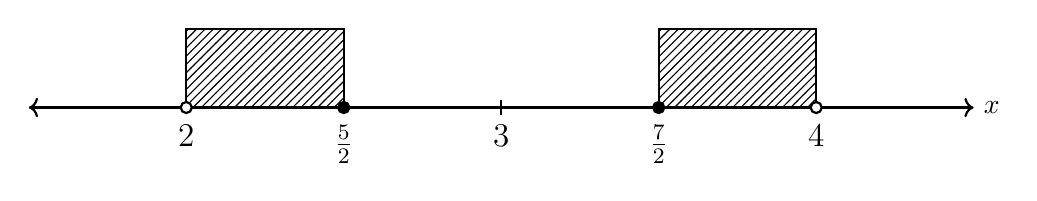
\begin{tikzpicture}
    \draw[thick,<->] (-6,0) -- (6,0) node[right] {$x$};
    \fill[pattern=north east lines] (-4,0) rectangle (-2,1);
    \fill[pattern=north east lines] (2,0) rectangle (4,1);
    \draw[thick] (-4,0) -- (-4,1) -- (-2,1) -- (-2,0);
    \draw[thick] (2,0) -- (2,1) -- (4,1) -- (4,0);
    \draw (-4,-0.1) node[below] {\large{$2$}};
    \draw (-2,-0.1) node[below] {\large{$\frac{5}{2}$}};
    \draw (0,-0.1) node[below] {\large{$3$}};
    \draw (2,-0.1) node[below] {\large{$\frac{7}{2}$}};
    \draw (4,-0.1) node[below] {\large{$4$}};
    \draw[thick] (0,-0.1) -- (0,0.1);
    \draw[fill=white, thick] (-4,0) circle (2pt);
    \draw[fill=black, thick] (-2,0) circle (2pt);
    \draw[fill=black, thick] (2,0) circle (2pt);
    \draw[fill=white, thick] (4,0) circle (2pt);
            \end{tikzpicture}
        \end{center}
        Sebagai pengecekan, untuk $x=\frac{9}{4}$ diperoleh $\frac{1}{|x-3|}=\frac{4}{3}$, dan berlaku $1<\frac{4}{3}\leq 2$. Jadi semua nilai $x$ yang memenuhi adalah $2<x\leq\frac{5}{2}$ atau $\frac{7}{2}\leq x<4$, atau dalam notasi interval $\colorlet{oldcolor}{.}
        \color{red}
        \setlength{\fboxrule}{1pt} \boxed{\color{oldcolor}\left(2,\frac{5}{2}\right]\cup\left[\frac{7}{2},4\right)}\color{oldcolor}$.
    }
    \end{jawab}

    \item Diberikan $f(x)=\sqrt{16-x^2}$ dan $g(x)=\dfrac{1}{x^2-4}$.
    \begin{enumerate}
        \item Dapatkan domain $f(x)$ dan $g(x)$.
        \item Dapatkan $(g\circ f)(x)$ dan domain $(g\circ f)(x)$.
    \end{enumerate}
    \begin{jawab}[domain fungsi, fungsi komposisi, domain fungsi komposisi]{
        \begin{enumerate}
            \item Diperhatikan bahwa $f(x)$ memuat akar kuadrat, sehingga syaratnya adalah $16-x^2\geq 0$, yaitu $(4-x)(4+x)\geq 0$ yang dipenuhi oleh $-4\leq x\leq 4$. Jadi
            \begin{align*}
                \colorlet{oldcolor}{.}
        \color{red}
        \setlength{\fboxrule}{1pt} \boxed{\color{oldcolor}D(f)=\{x\in\mathbb{R} : -4\leq x\leq 4\}=[-4,4]}\color{oldcolor}.
            \end{align*}
            Selanjutnya, $g(x)$ merupakan fungsi rasional, sehingga syaratnya adalah $x^2-4=(x-2)(x+2)\neq 0$. Jadi
            \begin{align*}
                \colorlet{oldcolor}{.}
        \color{red}
        \setlength{\fboxrule}{1pt} \boxed{\color{oldcolor}D(g)=\{x\in\mathbb{R} : x\neq -2,~x\neq 2\}=\mathbb{R}\setminus\{-2,2\}}\color{oldcolor}.
            \end{align*}
            \item Diperhatikan bahwa
            \begin{align*}
                (g\circ f)(x) = g(f(x)) = g\left(\sqrt{16-x^2}\right) = \frac{1}{\left(\sqrt{16-x^2}\right)^2-4} = \frac{1}{16-x^2-4} = \colorlet{oldcolor}{.}
        \color{red}
        \setlength{\fboxrule}{1pt} \boxed{\color{oldcolor}\frac{1}{12-x^2}}\color{oldcolor}.
            \end{align*}
            Domain dari fungsi komposisi $g\circ f$ adalah semua nilai $x$ pada domain $f$ sehingga nilai dari $f(x)$ berada pada domain $g$, yang dapat dirumuskan sebagai
            \begin{align*}
                \colorlet{oldcolor}{.}
        \color{blue}
        \setlength{\fboxrule}{1pt} \boxed{\color{oldcolor}D(g\circ f) = \{x \in D(f) : f(x) \in D(g)\} = \left\{x \in [-4,4] : \sqrt{16-x^2} \neq \pm 2\right\}}\color{oldcolor}.
            \end{align*}
            Karena $\sqrt{16-x^2}\geq 0$, maka $\sqrt{16-x^2}\neq -2$ selalu berlaku. Selanjutnya, $\sqrt{16-x^2}=2$ jika dan hanya jika $16-x^2=4$, yaitu $x^2=12$ atau $x=\pm 2\sqrt{3}$. Kedua nilai ini berada di $[-4,4]$ karena $2\sqrt{3}\approx 3{,}46$. Didapatkan
            \begin{align*}
                \colorlet{oldcolor}{.}
        \color{red}
        \setlength{\fboxrule}{1pt} \boxed{\color{oldcolor}D(g\circ f) = [-4,4]\setminus\left\{-2\sqrt{3},2\sqrt{3}\right\} = \left[-4,-2\sqrt{3}\right)\cup\left(-2\sqrt{3},2\sqrt{3}\right)\cup\left(2\sqrt{3},4\right]}\color{oldcolor}.
            \end{align*}
        \end{enumerate}
    }
    \end{jawab}

    \item Diberikan fungsi $f(x)=\left|\dfrac{x^2-4}{x+2}\right|$. Dapatkan titik $x$ di mana fungsi $f(x)$ diskontinu.\\
    Dapatkan nilai fungsi $f(x)$ pada titik tersebut agar menjadi kontinu dan sketsa grafik fungsi tersebut.
    \begin{jawab}[kekontinuan, diskontinuitas yang dapat dihapus, limit, nilai mutlak, sketsa grafik]{~\\
        Fungsi $f$ tidak terdefinisi saat penyebutnya nol, yaitu $x+2=0$ atau $x=-2$. Untuk $x\neq -2$, fungsi dapat disederhanakan menjadi
        \begin{align*}
            f(x) = \left|\frac{(x-2)(x+2)}{x+2}\right| = \colorlet{oldcolor}{.}
        \color{blue}
        \setlength{\fboxrule}{1pt} \boxed{\color{oldcolor}|x-2|}\color{oldcolor}, \quad x\neq -2.
        \end{align*}
        Fungsi $|x-2|$ kontinu di setiap bilangan real, sehingga satu-satunya titik diskontinu dari $f$ adalah titik di mana $f$ tidak terdefinisi, yaitu $\colorlet{oldcolor}{.}
        \color{red}
        \setlength{\fboxrule}{1pt} \boxed{\color{oldcolor}x=-2}\color{oldcolor}$.\\
        Selanjutnya, limit fungsi di titik tersebut adalah
        \begin{align*}
            \lim_{x\to -2} f(x) = \lim_{x\to -2} |x-2| = |-2-2| = 4.
        \end{align*}
        Karena limitnya ada, diskontinuitas di $x=-2$ dapat dihilangkan dengan mendefinisikan nilai fungsi di titik tersebut sama dengan limitnya, yaitu $\colorlet{oldcolor}{.}
        \color{red}
        \setlength{\fboxrule}{1pt} \boxed{\color{oldcolor}f(-2)=4}\color{oldcolor}$. Dengan definisi ini, $f(x)=|x-2|$ untuk setiap $x\in\mathbb{R}$, sehingga $f$ kontinu di mana-mana.\\
        Grafik $f$ sama dengan grafik $y=|x-2|$, yaitu grafik $y=|x|$ yang digeser $2$ satuan ke kanan, dengan titik puncak $(2,0)$. Pada fungsi semula, titik $(-2,4)$ berlubang (bulatan kosong), dan lubang tersebut tertutup setelah didefinisikan $f(-2)=4$. Sketsa grafiknya adalah sebagai berikut:
        \begin{center}
            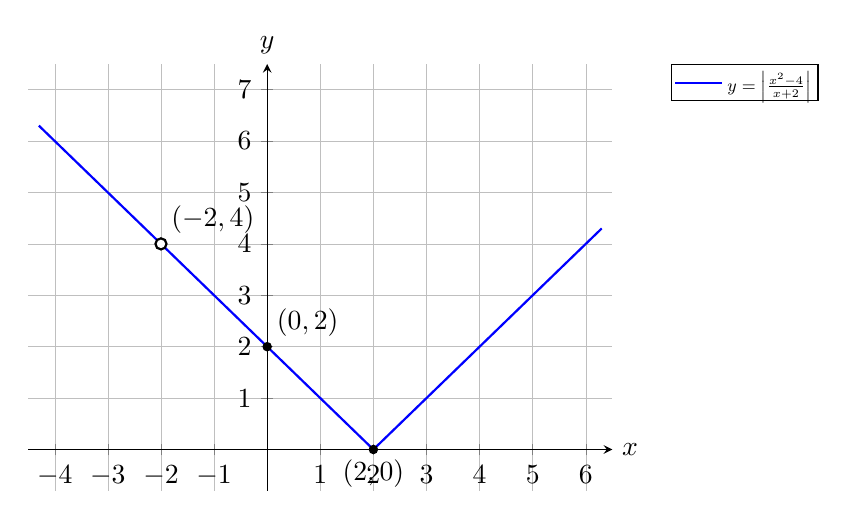
\begin{tikzpicture}
                \begin{axis}[
        axis lines = middle,
        xlabel = $x$,
        ylabel = {$y$},
        grid=both,
        grid style={line width=.1pt, draw=gray!10},
        major grid style={line width=.2pt,draw=gray!50},
        x label style={anchor=west}, % label x ke kanan
        y label style={anchor=south}, % label y ke atas
        samples=200,
        legend style={
                at={(1.1,1)},
                anchor=north west,
                font=\small,         % mengecilkan ukuran font
                row sep=1pt,         % jarak antar baris legend
                inner sep=1pt,       % margin dalam kotak legend
                nodes={scale=0.7}    % skalakan isi legend
            },
        xtick={-4,-3,...,6},
        ytick={0,1,...,7},
        xmin=-4.5, xmax=6.5,
        ymin=-0.8, ymax=7.5,
        width=9cm,
        height=7cm
    ]
\addplot[domain=-4.3:2, color=blue, thick, samples=2] {2-x};
\addlegendentry{$y=\left|\frac{x^2-4}{x+2}\right|$}
\addplot[domain=2:6.3, color=blue, thick, samples=2, forget plot] {x-2};
\draw[fill=white, thick] (-2,4) circle (2pt) node[above right] {$(-2,4)$};
\draw[fill=black] (2,0) circle (1.5pt) node[below] {$(2,0)$};
\draw[fill=black] (0,2) circle (1.5pt) node[above right] {$(0,2)$};
\end{axis}
            \end{tikzpicture}
        \end{center}
    }
    \end{jawab}

    \item Diberikan fungsi
    \begin{align*}
        f(x)=\begin{cases}
            \dfrac{x-16}{\sqrt{x}-4}, & x\neq 16\\
            7, & x=16
        \end{cases}.
    \end{align*}
    Selidiki kekontinuan $f(x)$ di $x=16$. Jika tidak kontinu, apakah diskontinuitasnya dapat dihilangkan? Jelaskan.
    \begin{jawab}[kekontinuan, limit fungsi, diskontinuitas yang dapat dihapus]{~\\
        Ingat kembali syarat fungsi kontinu di suatu titik \(x = a\) adalah
        \begin{enumerate}
            \item \(f(a)\) terdefinisi
            \item \(\displaystyle \lim_{x \to a} f(x)\) ada, yaitu $\displaystyle \lim_{x \to a^-} f(x) = \lim_{x \to a^+} f(x)$
            \item \(\displaystyle\lim_{x \to a} f(x) = f(a)\)
        \end{enumerate}
        Diperhatikan bahwa untuk $x=16$, $\colorlet{oldcolor}{.}
        \color{blue}
        \setlength{\fboxrule}{1pt} \boxed{\color{oldcolor}f(16) = 7~\text{terdefinisi}}\color{oldcolor}$. Selanjutnya, karena $x-16=(\sqrt{x})^2-4^2=(\sqrt{x}-4)(\sqrt{x}+4)$ untuk $x\geq 0$, limitnya adalah
        \begin{align*}
            \lim_{x\to 16} f(x) = \lim_{x\to 16} \frac{x-16}{\sqrt{x}-4} = \lim_{x\to 16} \frac{(\sqrt{x}-4)(\sqrt{x}+4)}{\sqrt{x}-4} = \lim_{x\to 16} (\sqrt{x}+4) = 4+4 = \colorlet{oldcolor}{.}
        \color{blue}
        \setlength{\fboxrule}{1pt} \boxed{\color{oldcolor}8}\color{oldcolor}.
        \end{align*}
        Syarat pertama dan kedua terpenuhi, tetapi $\displaystyle\lim_{x\to 16}f(x)=8\neq 7=f(16)$, sehingga syarat ketiga tidak terpenuhi. Jadi $\colorlet{oldcolor}{.}
        \color{red}
        \setlength{\fboxrule}{1pt} \boxed{\color{oldcolor}f \text{ tidak kontinu di } x=16}\color{oldcolor}$.\\
        Karena $\displaystyle\lim_{x\to 16}f(x)$ ada (bernilai $8$), maka diskontinuitas di $x=16$ $\colorlet{oldcolor}{.}
        \color{red}
        \setlength{\fboxrule}{1pt} \boxed{\color{oldcolor}\text{dapat dihilangkan}}\color{oldcolor}$, yaitu dengan mendefinisikan ulang nilai fungsi di titik tersebut menjadi $f(16)=8$. Dengan definisi baru ini, $f(x)=\sqrt{x}+4$ untuk setiap $x\geq 0$, dan $f$ kontinu di $x=16$.
    }
    \end{jawab}

    \item Dapatkan $f''(x)$ dimana $f(x)=x^2+\left(3-\sqrt{x}\right)^{-1}$.
    \begin{jawab}[turunan kedua, aturan rantai, aturan perkalian]{~\\
        Fungsi $f$ terdefinisi untuk $x\geq 0$ dan $x\neq 9$, dan turunannya ada untuk $x>0$, $x\neq 9$. Ingat kembali aturan rantai, yaitu $\colorlet{oldcolor}{.}
        \color{blue}
        \setlength{\fboxrule}{1pt} \boxed{\color{oldcolor}\frac{d}{dx}[h(g(x))] = h'(g(x)) \cdot g'(x)}\color{oldcolor}$, serta $\frac{d}{dx}\left(\sqrt{x}\right)=\frac{1}{2\sqrt{x}}$. Turunan pertama dari $f$ adalah
        \begin{align*}
            f'(x) &= 2x + (-1)\left(3-\sqrt{x}\right)^{-2}\cdot\left(-\frac{1}{2\sqrt{x}}\right)\\
            &= \colorlet{oldcolor}{.}
        \color{blue}
        \setlength{\fboxrule}{1pt} \boxed{\color{oldcolor}2x + \frac{1}{2}x^{-1/2}\left(3-\sqrt{x}\right)^{-2}}\color{oldcolor}.
        \end{align*}
        Untuk turunan kedua, suku kedua diturunkan dengan aturan perkalian $(uv)'=u'v+uv'$, dengan $u=x^{-1/2}$ dan $v=\left(3-\sqrt{x}\right)^{-2}$, sehingga
        \begin{align*}
            \colorlet{oldcolor}{.}
        \color{blue}
        \setlength{\fboxrule}{1pt} \boxed{\color{oldcolor}u'=-\frac{1}{2}x^{-3/2}}\color{oldcolor} \quad\text{dan}\quad \colorlet{oldcolor}{.}
        \color{blue}
        \setlength{\fboxrule}{1pt} \boxed{\color{oldcolor}v'=-2\left(3-\sqrt{x}\right)^{-3}\cdot\left(-\frac{1}{2\sqrt{x}}\right)=x^{-1/2}\left(3-\sqrt{x}\right)^{-3}}\color{oldcolor}.
        \end{align*}
        Dengan demikian, diperoleh
        \begin{align*}
            f''(x) &= 2 + \frac{1}{2}\left[-\frac{1}{2}x^{-3/2}\left(3-\sqrt{x}\right)^{-2} + x^{-1/2}\cdot x^{-1/2}\left(3-\sqrt{x}\right)^{-3}\right]\\
            &= 2 - \frac{1}{4x\sqrt{x}\left(3-\sqrt{x}\right)^{2}} + \frac{1}{2x\left(3-\sqrt{x}\right)^{3}}\\
            &= 2 + \frac{-\left(3-\sqrt{x}\right) + 2\sqrt{x}}{4x\sqrt{x}\left(3-\sqrt{x}\right)^{3}}\\
            &= \colorlet{oldcolor}{.}
        \color{red}
        \setlength{\fboxrule}{1pt} \boxed{\color{oldcolor}2 + \frac{3\left(\sqrt{x}-1\right)}{4x\sqrt{x}\left(3-\sqrt{x}\right)^{3}}}\color{oldcolor}, \quad x>0,~x\neq 9.
        \end{align*}
    }
    \end{jawab}
\end{enumerate}

\newpage

%%%%%%%%%%%%%%%%%%%%%%%%%%%%%%%%%%%%%%%%%%%%%%%%%%%%%%%%%%%%%%%%%%%%%%%%%%%%%%
% Kal-1
\kopsoal{Kal-1}{1-6}{Fisika, T. Kimia, T. Pangan}{Selasa, Kamis; 12.30-15.00}{8}
\begin{enumerate}
    \item Selesaikan pertidaksamaan berikut
    \begin{align*}
        \frac{1}{x-3}\leq\frac{2}{x+1}.
    \end{align*}
    \begin{jawab}[pertidaksamaan rasional, pecahan, garis bilangan, notasi interval]{~\\
        Untuk menyelesaikan pertidaksamaan rasional, pastikan ruas kanan sudah bernilai nol (jangan dikali silang, karena tanda penyebutnya belum diketahui). Dengan mengurangkan \(\frac{2}{x+1}\) dari kedua ruas, didapatkan
        \[
        \frac{1}{x-3} - \frac{2}{x+1} \leq 0
        \]
        Selanjutnya, dengan menyamakan penyebut dan menyederhanakan bentuknya, diperoleh
        \begin{align}
            \frac{(x+1)-2(x-3)}{(x-3)(x+1)} &\leq 0\nonumber\\
            \frac{x+1-2x+6}{(x-3)(x+1)} &\leq 0\nonumber \\
            \frac{7-x}{(x-3)(x+1)} &\leq 0 \label{ineq:kal1}
        \end{align}
        Didapatkan pembuat nol dari faktor-faktornya adalah
        \begin{align*}
            7-x = 0 \quad &\vee\quad  x-3 = 0 \quad\vee\quad x+1=0\\
            \colorlet{oldcolor}{.}
        \color{blue}
        \setlength{\fboxrule}{1pt} \boxed{\color{oldcolor}x=7}\color{oldcolor} \quad &\vee\quad \colorlet{oldcolor}{.}
        \color{blue}
        \setlength{\fboxrule}{1pt} \boxed{\color{oldcolor}x=3}\color{oldcolor} \quad\vee\quad \colorlet{oldcolor}{.}
        \color{blue}
        \setlength{\fboxrule}{1pt} \boxed{\color{oldcolor}x=-1}\color{oldcolor}
        \end{align*}
        Selanjutnya, dibuat garis bilangan dan dilakukan uji titik pada ekspresi \eqref{ineq:kal1} sebagai berikut
        \begin{itemize}
            \item Untuk \(x < -1\), misalkan \(x = -2\):
            \[
            \frac{7-(-2)}{(-2-3)(-2+1)} = \frac{9}{(-5)(-1)} = \frac{9}{5} > 0
            \]
            \item Untuk \(-1 < x < 3\), misalkan \(x = 0\):
            \[
            \frac{7-0}{(0-3)(0+1)} = \frac{7}{-3} < 0
            \]
            \item Untuk \(3 < x < 7\), misalkan \(x = 4\):
            \[
            \frac{7-4}{(4-3)(4+1)} = \frac{3}{5} > 0
            \]
            \item Untuk \(x > 7\), misalkan \(x = 8\):
            \[
            \frac{7-8}{(8-3)(8+1)} = \frac{-1}{45} < 0
            \]
        \end{itemize}
        \begin{center}
           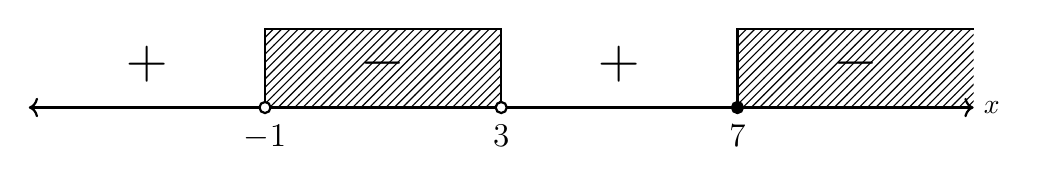
\begin{tikzpicture}
    \draw[thick,<->] (-6,0) -- (6,0) node[right] {$x$};
    \fill[pattern=north east lines] (-3,0) rectangle (0,1);
    \fill[pattern=north east lines] (3,0) rectangle (6,1);
    \draw[thick] (-3,0) -- (-3,1) -- (0,1) -- (0,0);
    \draw[thick] (3,0) -- (3,1) -- (6,1);
    \draw (-3,-0.1) node[below] {\large{$-1$}};
    \draw (0,-0.1) node[below] {\large{$3$}};
    \draw (3,-0.1) node[below] {\large{$7$}};
    \draw (-4.5,0.2) node[above] {\huge{$+$}};
    \draw (-1.5,0.2) node[above] {\huge{$-$}};
    \draw (1.5,0.2) node[above] {\huge{$+$}};
    \draw (4.5,0.2) node[above] {\huge{$-$}};
    \draw[fill=white, thick] (-3,0) circle (2pt);
    \draw[fill=white, thick] (0,0) circle (2pt);
    \draw[fill=black, thick] (3,0) circle (2pt);
\end{tikzpicture}
        \end{center}
        Karena yang diminta adalah nilai \(x\) yang membuat pertidaksamaan \eqref{ineq:kal1} kurang dari atau sama dengan nol, diambil interval yang bertanda negatif beserta pembuat nol pembilang ($x=7$). Pembuat nol penyebut ($x=-1$ dan $x=3$) tidak diikutkan karena membuat ekspresi tidak terdefinisi. Jadi solusi dari pertidaksamaan tersebut adalah \(-1 < x < 3\) atau \(x\geq 7\). Dalam notasi interval, solusi tersebut dapat ditulis sebagai $\colorlet{oldcolor}{.}
        \color{red}
        \setlength{\fboxrule}{1pt} \boxed{\color{oldcolor}(-1, 3)\cup[7,\infty)}\color{oldcolor}$.
    }
    \end{jawab}

    \item Diberikan fungsi $f(x)=\dfrac{1}{x-3}$ dan $g(x)=\sqrt{7-x}$. Tentukan:
    \begin{enumerate}
        \item Domain fungsi $f$ dan $g$.
        \item Fungsi $(f\circ g)(x)$ dan $\left(\dfrac{f}{g}\right)(x)$ beserta domainnya masing-masing.
    \end{enumerate}
    \begin{jawab}[domain fungsi, fungsi komposisi, operasi pembagian fungsi, domain fungsi]{
        \begin{enumerate}
            \item Diperhatikan bahwa $f(x)$ merupakan fungsi rasional, sehingga domainnya adalah semua bilangan real kecuali nilai yang membuat penyebutnya sama dengan nol, yaitu $x-3\neq 0$. Jadi
            \[
            \colorlet{oldcolor}{.}
        \color{red}
        \setlength{\fboxrule}{1pt} \boxed{\color{oldcolor}D(f)=\{x \in \mathbb{R} : x \neq 3\}}\color{oldcolor}.
            \]
            Selanjutnya, diperhatikan bahwa $g(x)$ memuat akar kuadrat, sehingga domainnya adalah semua bilangan real yang membuat ekspresi di dalam akar kuadrat tak negatif, yaitu $7-x\geq 0$. Jadi
            \[
            \colorlet{oldcolor}{.}
        \color{red}
        \setlength{\fboxrule}{1pt} \boxed{\color{oldcolor}D(g)=\{x \in \mathbb{R} : x \leq 7\}=(-\infty,7]}\color{oldcolor}.
            \]
            \item Diperhatikan bahwa
            \begin{align*}
                (f\circ g)(x) = f(g(x)) = f\left(\sqrt{7-x}\right) = \colorlet{oldcolor}{.}
        \color{red}
        \setlength{\fboxrule}{1pt} \boxed{\color{oldcolor}\frac{1}{\sqrt{7-x} - 3}}\color{oldcolor}
            \end{align*}
            Domain dari fungsi komposisi $f\circ g$ adalah semua nilai $x$ pada domain $g$ sehingga nilai dari $g(x)$ berada pada domain $f$, yang dapat dirumuskan sebagai
            \begin{align*}
                \colorlet{oldcolor}{.}
        \color{blue}
        \setlength{\fboxrule}{1pt} \boxed{\color{oldcolor}D(f\circ g) = \{x \in D(g) : g(x) \in D(f)\} = \left\{x \in (-\infty, 7] : \sqrt{7-x} \neq 3\right\}}\color{oldcolor}.
            \end{align*}
            Karena $\sqrt{7-x} = 3$ jika dan hanya jika $7-x = 9$, yang berarti $x = -2$, didapatkan
            \begin{align*}
                \colorlet{oldcolor}{.}
        \color{red}
        \setlength{\fboxrule}{1pt} \boxed{\color{oldcolor}D(f\circ g) = (-\infty, 7] \setminus \{-2\} = (-\infty, -2) \cup (-2, 7]}\color{oldcolor}.
            \end{align*}
            Selanjutnya, untuk pembagian fungsi diperoleh
            \begin{align*}
                \left(\frac{f}{g}\right)(x) = \frac{f(x)}{g(x)} = \frac{\frac{1}{x-3}}{\sqrt{7-x}} = \colorlet{oldcolor}{.}
        \color{red}
        \setlength{\fboxrule}{1pt} \boxed{\color{oldcolor}\frac{1}{(x-3)\sqrt{7-x}}}\color{oldcolor}.
            \end{align*}
            Domain dari $\frac{f}{g}$ adalah irisan domain $f$ dan $g$, dikurangi nilai $x$ yang membuat $g(x)=0$, yaitu
            \begin{align*}
                \colorlet{oldcolor}{.}
        \color{blue}
        \setlength{\fboxrule}{1pt} \boxed{\color{oldcolor}D\left(\frac{f}{g}\right) = \{x \in D(f)\cap D(g) : g(x) \neq 0\}}\color{oldcolor}.
            \end{align*}
            Karena $D(f)\cap D(g) = (-\infty,3)\cup(3,7]$ dan $g(x)=\sqrt{7-x}=0$ jika dan hanya jika $x=7$, didapatkan
            \begin{align*}
                \colorlet{oldcolor}{.}
        \color{red}
        \setlength{\fboxrule}{1pt} \boxed{\color{oldcolor}D\left(\frac{f}{g}\right) = (-\infty, 3) \cup (3, 7)}\color{oldcolor}.
            \end{align*}
        \end{enumerate}
    }
    \end{jawab}

    \item Diketahui $f(x)=\sqrt{9-x^2}$.
    \begin{enumerate}
        \item Tentukan domain $f(x)$.
        \item Apakah $f^{-1}(x)$ ada? Jelaskan alasannya.
        \item Jika tidak ada, definisikan domain $f(x)$ agar $f^{-1}(x)$ ada, kemudian dapatkan $f^{-1}(x)$ beserta domainnya.
    \end{enumerate}
    \begin{jawab}[domain fungsi, fungsi satu-satu, fungsi invers]{
        \begin{enumerate}
            \item Diperhatikan bahwa $f(x)$ memuat akar kuadrat, sehingga syaratnya adalah $9-x^2\geq 0$, yaitu $(3-x)(3+x)\geq 0$ yang dipenuhi oleh $-3\leq x\leq 3$. Jadi
            \begin{align*}
                \colorlet{oldcolor}{.}
        \color{red}
        \setlength{\fboxrule}{1pt} \boxed{\color{oldcolor}D(f)=\{x\in\mathbb{R} : -3\leq x\leq 3\}=[-3,3]}\color{oldcolor}.
            \end{align*}
            \item Suatu fungsi mempunyai invers jika fungsi tersebut satu-satu (injektif), yaitu setiap nilai $y$ hanya dicapai oleh tepat satu nilai $x$. Diperhatikan bahwa grafik $f$ adalah setengah lingkaran atas $x^2+y^2=9$, dan misalnya
            \begin{align*}
                f(-3)=\sqrt{9-9}=0=f(3) \quad\text{padahal}\quad -3\neq 3.
            \end{align*}
            Jadi $f$ tidak satu-satu pada $[-3,3]$, sehingga $\colorlet{oldcolor}{.}
        \color{red}
        \setlength{\fboxrule}{1pt} \boxed{\color{oldcolor}f^{-1}(x) \text{ tidak ada}}\color{oldcolor}$ (secara grafik, garis mendatar $y=c$ dengan $0\leq c<3$ memotong grafik di dua titik).
            \item Agar $f$ satu-satu, domain $f$ dibatasi pada salah satu sisi sumbu-$y$, misalnya $\colorlet{oldcolor}{.}
        \color{blue}
        \setlength{\fboxrule}{1pt} \boxed{\color{oldcolor}D(f)=[0,3]}\color{oldcolor}$. Pada domain ini, $f$ turun dari $f(0)=3$ sampai $f(3)=0$, sehingga $R(f)=[0,3]$.\\
            Misalkan $y=f(x)$ dengan $x\in[0,3]$, kemudian selesaikan sehingga terbentuk $x$ dalam fungsi $y$. Diperoleh
            \begin{align*}
                y &= \sqrt{9-x^2}\\
                y^2 &= 9-x^2\\
                x^2 &= 9-y^2\\
                x &= \sqrt{9-y^2} \quad (\text{karena } x\geq 0).
            \end{align*}
            Dari sini didapatkan $x = f^{-1}(y) = \sqrt{9-y^2}$. Dengan mengganti $y$ dengan $x$, dan mengingat bahwa domain dari fungsi invers adalah range dari fungsi asli, diperoleh
            \begin{align*}
                \colorlet{oldcolor}{.}
        \color{red}
        \setlength{\fboxrule}{1pt} \boxed{\color{oldcolor}f^{-1}(x)=\sqrt{9-x^2},\quad D(f^{-1})=R(f)=[0,3]}\color{oldcolor}.
            \end{align*}
            Menariknya, pada domain $[0,3]$ fungsi invers ini sama dengan fungsi asalnya, karena grafik seperempat lingkaran tersebut simetris terhadap garis $y=x$.\\
            \textit{Catatan:} jika dipilih domain $[-3,0]$, maka diperoleh $f^{-1}(x)=-\sqrt{9-x^2}$ dengan domain $[0,3]$.
        \end{enumerate}
    }
    \end{jawab}

    \item Diberikan fungsi
    \begin{align*}
        f(x)=\begin{cases}
            \dfrac{9-x}{3-\sqrt{x}}, & x\neq 9\\
            k, & x=9
        \end{cases},\quad \text{dengan } x\in[0,\infty).
    \end{align*}
    \begin{enumerate}
        \item Tentukan nilai $k$ sehingga $f(x)$ kontinu di $x=9$.
        \item Untuk nilai $k$ tersebut, nyatakan $f(x)$ tanpa menggunakan bentuk fungsi sepotong-sepotong.
    \end{enumerate}
    \begin{jawab}[fungsi kontinu, limit fungsi, fungsi sepotong-sepotong]{
        \begin{enumerate}
            \item Ingat kembali syarat fungsi kontinu di suatu titik \(x = a\) adalah
            \begin{enumerate}
                \item \(f(a)\) terdefinisi
                \item \(\displaystyle \lim_{x \to a} f(x)\) ada, yaitu $\displaystyle \lim_{x \to a^-} f(x) = \lim_{x \to a^+} f(x)$
                \item \(\displaystyle\lim_{x \to a} f(x) = f(a)\)
            \end{enumerate}
            Diperhatikan bahwa untuk \(x = 9\), \(\colorlet{oldcolor}{.}
        \color{blue}
        \setlength{\fboxrule}{1pt} \boxed{\color{oldcolor}f(9) = k~\text{terdefinisi}}\color{oldcolor}\). Karena untuk $x\geq 0$ berlaku $9-x=3^2-(\sqrt{x})^2=(3-\sqrt{x})(3+\sqrt{x})$, didapatkan limitnya adalah
            \begin{align*}
            \lim_{x \to 9} f(x) = \lim_{x \to 9} \frac{9-x}{3-\sqrt{x}} = \lim_{x \to 9} \frac{(3-\sqrt{x})(3+\sqrt{x})}{3-\sqrt{x}} = \lim_{x \to 9} (3+\sqrt{x}) = 3+3 = \colorlet{oldcolor}{.}
        \color{blue}
        \setlength{\fboxrule}{1pt} \boxed{\color{oldcolor}6}\color{oldcolor}.
            \end{align*}
            Selanjutnya, untuk syarat ketiga, haruslah $\displaystyle \colorlet{oldcolor}{.}
        \color{blue}
        \setlength{\fboxrule}{1pt} \boxed{\color{oldcolor}\lim_{x \to 9} f(x) = f(9)}\color{oldcolor}$, sehingga diperoleh $\colorlet{oldcolor}{.}
        \color{red}
        \setlength{\fboxrule}{1pt} \boxed{\color{oldcolor}k=6}\color{oldcolor}$.
            \item Diperhatikan bahwa untuk $x\in[0,\infty)$ dengan $x\neq 9$ berlaku $f(x)=3+\sqrt{x}$ (dari proses perhitungan limit di atas), dan untuk $x=9$ nilai $3+\sqrt{9}=6=k=f(9)$. Dengan demikian, fungsi $f(x)$ dapat dinyatakan tanpa bentuk sepotong-sepotong sebagai
            \begin{align*}
                \colorlet{oldcolor}{.}
        \color{red}
        \setlength{\fboxrule}{1pt} \boxed{\color{oldcolor}f(x) = 3+\sqrt{x}, \quad x \in [0,\infty)}\color{oldcolor}.
            \end{align*}
        \end{enumerate}
    }
    \end{jawab}

    \item Dapatkan $f''(x)$ dimana $f(x)=3x+\left(2\sqrt{x}+1\right)^{-1}$.
    \begin{jawab}[turunan kedua, aturan rantai, aturan perkalian]{~\\
        Fungsi $f$ terdefinisi untuk $x\geq 0$, dan turunannya ada untuk $x>0$. Ingat kembali aturan rantai, yaitu $\colorlet{oldcolor}{.}
        \color{blue}
        \setlength{\fboxrule}{1pt} \boxed{\color{oldcolor}\frac{d}{dx}[h(g(x))] = h'(g(x)) \cdot g'(x)}\color{oldcolor}$, serta $\frac{d}{dx}\left(2\sqrt{x}\right)=\frac{1}{\sqrt{x}}$. Turunan pertama dari $f$ adalah
        \begin{align*}
            f'(x) &= 3 + (-1)\left(2\sqrt{x}+1\right)^{-2}\cdot\frac{1}{\sqrt{x}}\\
            &= \colorlet{oldcolor}{.}
        \color{blue}
        \setlength{\fboxrule}{1pt} \boxed{\color{oldcolor}3 - x^{-1/2}\left(2\sqrt{x}+1\right)^{-2}}\color{oldcolor}.
        \end{align*}
        Untuk turunan kedua, suku kedua diturunkan dengan aturan perkalian $(uv)'=u'v+uv'$, dengan $u=x^{-1/2}$ dan $v=\left(2\sqrt{x}+1\right)^{-2}$, sehingga
        \begin{align*}
            \colorlet{oldcolor}{.}
        \color{blue}
        \setlength{\fboxrule}{1pt} \boxed{\color{oldcolor}u'=-\frac{1}{2}x^{-3/2}}\color{oldcolor} \quad\text{dan}\quad \colorlet{oldcolor}{.}
        \color{blue}
        \setlength{\fboxrule}{1pt} \boxed{\color{oldcolor}v'=-2\left(2\sqrt{x}+1\right)^{-3}\cdot\frac{1}{\sqrt{x}}=-2x^{-1/2}\left(2\sqrt{x}+1\right)^{-3}}\color{oldcolor}.
        \end{align*}
        Dengan demikian, diperoleh
        \begin{align*}
            f''(x) &= 0 - \left[-\frac{1}{2}x^{-3/2}\left(2\sqrt{x}+1\right)^{-2} - 2x^{-1/2}\cdot x^{-1/2}\left(2\sqrt{x}+1\right)^{-3}\right]\\
            &= \frac{1}{2x\sqrt{x}\left(2\sqrt{x}+1\right)^{2}} + \frac{2}{x\left(2\sqrt{x}+1\right)^{3}}\\
            &= \frac{\left(2\sqrt{x}+1\right) + 4\sqrt{x}}{2x\sqrt{x}\left(2\sqrt{x}+1\right)^{3}}\\
            &= \colorlet{oldcolor}{.}
        \color{red}
        \setlength{\fboxrule}{1pt} \boxed{\color{oldcolor}\frac{6\sqrt{x}+1}{2x\sqrt{x}\left(2\sqrt{x}+1\right)^{3}}}\color{oldcolor}, \quad x>0.
        \end{align*}
    }
    \end{jawab}
\end{enumerate}

\newpage

%%%%%%%%%%%%%%%%%%%%%%%%%%%%%%%%%%%%%%%%%%%%%%%%%%%%%%%%%%%%%%%%%%%%%%%%%%%%%%
% Kal-2
\kopsoal{Kal-2}{7-12}{T. Lingkungan, T. Elektro, T. Biomedik}{Selasa, Kamis; 12.30-15.00}{8}
\begin{enumerate}
    \item Diberikan garis $\ell$ melalui titik $(3,2)$ dan $(a,b)$ dengan kemiringan $2$, dan garis $k$ melalui titik $(0,-1)$ dan $(a,b)$ dengan kemiringan $-1$. Dapatkan nilai $a$ dan $b$.
    \begin{jawab}[kemiringan garis, persamaan garis, sistem persamaan linear]{~\\
        Kemiringan garis yang melalui dua titik $(x_1,y_1)$ dan $(x_2,y_2)$ adalah $\colorlet{oldcolor}{.}
        \color{blue}
        \setlength{\fboxrule}{1pt} \boxed{\color{oldcolor}m = \frac{y_2 - y_1}{x_2 - x_1}}\color{oldcolor}$.
        \begin{itemize}
            \item Garis $\ell$ melalui $(3,2)$ dan $(a,b)$ dengan kemiringan $2$, sehingga
            \begin{align*}
                \frac{b-2}{a-3} = 2 \implies b-2 = 2a-6 \implies \colorlet{oldcolor}{.}
        \color{blue}
        \setlength{\fboxrule}{1pt} \boxed{\color{oldcolor}b = 2a-4}\color{oldcolor}.
            \end{align*}
            \item Garis $k$ melalui $(0,-1)$ dan $(a,b)$ dengan kemiringan $-1$, sehingga
            \begin{align*}
                \frac{b-(-1)}{a-0} = -1 \implies b+1 = -a \implies \colorlet{oldcolor}{.}
        \color{blue}
        \setlength{\fboxrule}{1pt} \boxed{\color{oldcolor}b = -a-1}\color{oldcolor}.
            \end{align*}
        \end{itemize}
        Dengan menyamakan kedua persamaan tersebut, diperoleh
        \begin{align*}
            2a-4 = -a-1 \implies 3a = 3 \implies a = 1,
        \end{align*}
        dan $b=2(1)-4=-2$. Sebagai pengecekan, kemiringan dari $(3,2)$ ke $(1,-2)$ adalah $\frac{-2-2}{1-3}=2$, dan kemiringan dari $(0,-1)$ ke $(1,-2)$ adalah $\frac{-2+1}{1-0}=-1$. Jadi $\colorlet{oldcolor}{.}
        \color{red}
        \setlength{\fboxrule}{1pt} \boxed{\color{oldcolor}a=1 \text{ dan } b=-2}\color{oldcolor}$, yaitu titik $(a,b)=(1,-2)$ merupakan titik potong kedua garis.
    }
    \end{jawab}

    \item Gambarkan kurva dasar $y=\dfrac{1}{x}$. Berdasarkan kurva dasar tersebut, gunakan translasi (pergeseran) untuk menggambar kurva $y=\dfrac{1}{x+1}-2$ (Jelaskan ilustrasinya).
    \begin{jawab}[fungsi rasional, asimtot, translasi grafik]{~\\
        Kurva dasar $y=\frac{1}{x}$ merupakan hiperbola yang terletak di kuadran I dan III, dengan asimtot tegak $x=0$ (sumbu-$y$) dan asimtot datar $y=0$ (sumbu-$x$). Kurva ini melalui titik-titik seperti $(1,1)$, $\left(2,\frac{1}{2}\right)$, $(-1,-1)$, dan $\left(-2,-\frac{1}{2}\right)$.\\
        Ingat kembali bahwa mengganti $x$ dengan $x+1$ berarti menggeser grafik sejauh $1$ satuan ke kiri, dan menambahkan konstanta $-2$ pada $y$ berarti menggeser grafik sejauh $2$ satuan ke bawah. Dengan demikian, proses translasinya adalah sebagai berikut.
        \begin{enumerate}
            \item[(i)] Gambar kurva dasar $y=\frac{1}{x}$ dengan asimtot $x=0$ dan $y=0$.
            \item[(ii)] Geser kurva $y=\frac{1}{x}$ sejauh $1$ satuan ke kiri, sehingga diperoleh kurva $y=\frac{1}{x+1}$ dengan asimtot tegak $x=-1$ dan asimtot datar $y=0$.
            \item[(iii)] Geser kurva $y=\frac{1}{x+1}$ sejauh $2$ satuan ke bawah, sehingga diperoleh kurva $y=\frac{1}{x+1}-2$ dengan asimtot tegak $\colorlet{oldcolor}{.}
        \color{blue}
        \setlength{\fboxrule}{1pt} \boxed{\color{oldcolor}x=-1}\color{oldcolor}$ dan asimtot datar $\colorlet{oldcolor}{.}
        \color{blue}
        \setlength{\fboxrule}{1pt} \boxed{\color{oldcolor}y=-2}\color{oldcolor}$.
        \end{enumerate}
        Sebagai bantuan, titik potong kurva dengan sumbu-$y$ ($x=0$) adalah $y=1-2=-1$, yaitu titik $(0,-1)$, sedangkan titik potong dengan sumbu-$x$ ($y=0$) adalah $\frac{1}{x+1}=2$, yaitu $x=-\frac{1}{2}$. Titik $(1,1)$ pada kurva dasar berpindah ke titik $(0,-1)$. Sketsa grafiknya adalah sebagai berikut.
        \begin{center}
            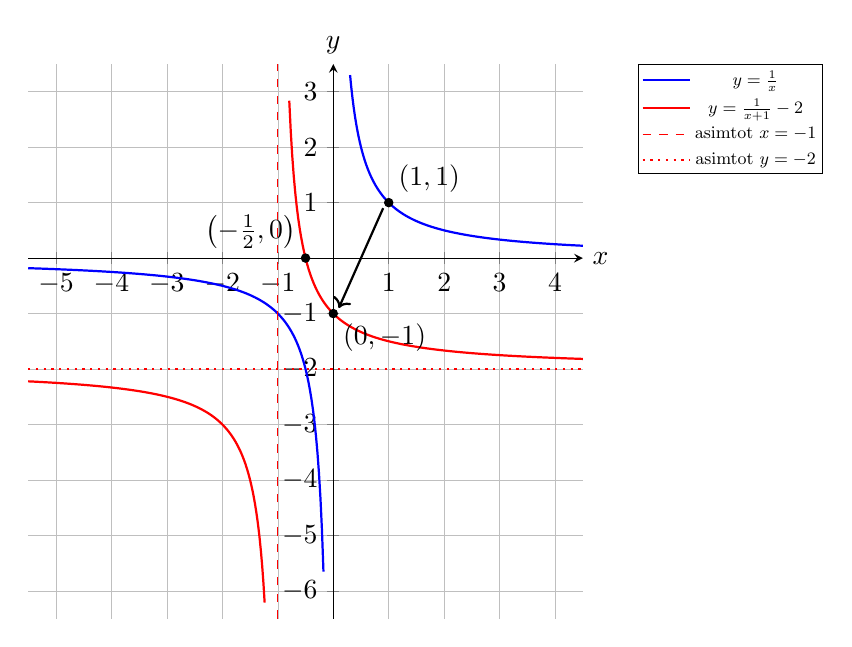
\begin{tikzpicture}
                \begin{axis}[
        axis lines = middle,
        xlabel = $x$,
        ylabel = {$y$},
        grid=both,
        grid style={line width=.1pt, draw=gray!10},
        major grid style={line width=.2pt,draw=gray!50},
        x label style={anchor=west}, % label x ke kanan
        y label style={anchor=south}, % label y ke atas
        samples=200,
        legend style={
                at={(1.1,1)},
                anchor=north west,
                font=\small,         % mengecilkan ukuran font
                row sep=1pt,         % jarak antar baris legend
                inner sep=1pt,       % margin dalam kotak legend
                nodes={scale=0.7}    % skalakan isi legend
            },
        xtick={-5,-4,...,4},
        ytick={-6,-5,...,3},
        xmin=-5.5, xmax=4.5,
        ymin=-6.5, ymax=3.5,
        axis equal image,
        width=10cm,
        restrict y to domain=-6.5:3.5
    ]
\addplot[domain=-5.5:-0.15, color=blue, thick] {1/x};
\addlegendentry{$y=\frac{1}{x}$}
\addplot[domain=0.15:4.5, color=blue, thick, forget plot] {1/x};
\addplot[domain=-5.5:-1.15, color=red, thick] {1/(x+1)-2};
\addlegendentry{$y=\frac{1}{x+1}-2$}
\addplot[domain=-0.82:4.5, color=red, thick, forget plot] {1/(x+1)-2};
\addplot[color=red, dashed] coordinates {(-1,-6.5) (-1,3.5)};
\addlegendentry{asimtot $x=-1$}
\addplot[color=red, dotted, thick] coordinates {(-5.5,-2) (4.5,-2)};
\addlegendentry{asimtot $y=-2$}
\draw[fill=black] (1,1) circle (1.5pt) node[above right] {$(1,1)$};
\draw[fill=black] (0,-1) circle (1.5pt) node[below right] {$(0,-1)$};
\draw[fill=black] (-0.5,0) circle (1.5pt) node[above left] {$\left(-\frac{1}{2},0\right)$};
\draw[->, thick] (0.9,0.9) -- (0.1,-0.9);
\end{axis}
            \end{tikzpicture}
        \end{center}
        Jadi kurva $y=\frac{1}{x+1}-2$ adalah
        \[\colorlet{oldcolor}{.}
        \color{red}
        \setlength{\fboxrule}{1pt} \boxed{\color{oldcolor}\text{hiperbola } y=\tfrac{1}{x} \text{ yang digeser 1 satuan ke kiri dan 2 satuan ke bawah}}\color{oldcolor}.\]
    }
    \end{jawab}

    \item Diberikan fungsi $f(x)=\sqrt[3]{x-1}+3$.
    \begin{enumerate}
        \item Dapatkan $f^{-1}(x)$.
        \item Dapatkan domain dan range dari $f^{-1}(x)$.
        \item Sketsa grafik dari $f(x)$ dan $f^{-1}(x)$ pada satu bidang koordinat.
    \end{enumerate}
    \begin{jawab}[fungsi invers, domain dan range, sketsa grafik fungsi invers]{
        \begin{enumerate}
            \item Untuk mendapatkan fungsi invers dari $f(x)$, kita misalkan $y=f(x)$, kemudian selesaikan sehingga terbentuk $x$ dalam fungsi $y$. Diperoleh
            \begin{align*}
                y &= \sqrt[3]{x-1}+3\\
                y-3 &= \sqrt[3]{x-1}\\
                (y-3)^3 &= x-1\\
                x &= (y-3)^3+1.
            \end{align*}
            Dari sini didapatkan $x = f^{-1}(y) = (y-3)^3+1$. Dengan mengganti $y$ dengan $x$, diperoleh
            \begin{align*}
                \colorlet{oldcolor}{.}
        \color{red}
        \setlength{\fboxrule}{1pt} \boxed{\color{oldcolor}f^{-1}(x) = (x-3)^3+1}\color{oldcolor}.
            \end{align*}
            \item Akar pangkat tiga terdefinisi untuk setiap bilangan real (termasuk bilangan negatif), sehingga $D(f)=\mathbb{R}$, dan nilai $\sqrt[3]{x-1}$ dapat mencapai sebarang bilangan real, sehingga $R(f)=\mathbb{R}$. Domain dari fungsi invers adalah range dari fungsi asli dan range dari fungsi invers adalah domain dari fungsi asli, yaitu
            \begin{align*}
                \colorlet{oldcolor}{.}
        \color{red}
        \setlength{\fboxrule}{1pt} \boxed{\color{oldcolor}D(f^{-1}) = R(f) = \mathbb{R}}\color{oldcolor} \quad\text{dan}\quad \colorlet{oldcolor}{.}
        \color{red}
        \setlength{\fboxrule}{1pt} \boxed{\color{oldcolor}R(f^{-1}) = D(f) = \mathbb{R}}\color{oldcolor}.
            \end{align*}
            Hal ini sesuai dengan $f^{-1}(x)=(x-3)^3+1$ yang merupakan fungsi polinomial.
            \item Grafik $f$ adalah grafik $y=\sqrt[3]{x}$ yang digeser $1$ satuan ke kanan dan $3$ satuan ke atas, dengan titik belok $(1,3)$. Grafik $f^{-1}$ adalah grafik $y=x^3$ yang digeser $3$ satuan ke kanan dan $1$ satuan ke atas, dengan titik belok $(3,1)$, dan merupakan pencerminan grafik $f$ terhadap garis $y=x$. Sebagai bantuan, grafik $f$ melalui titik $(0,2)$, $(1,3)$, $(2,4)$, dan $(9,5)$, sehingga grafik $f^{-1}$ melalui titik $(2,0)$, $(3,1)$, $(4,2)$, dan $(5,9)$. Sketsa grafiknya adalah sebagai berikut.
            \begin{center}
                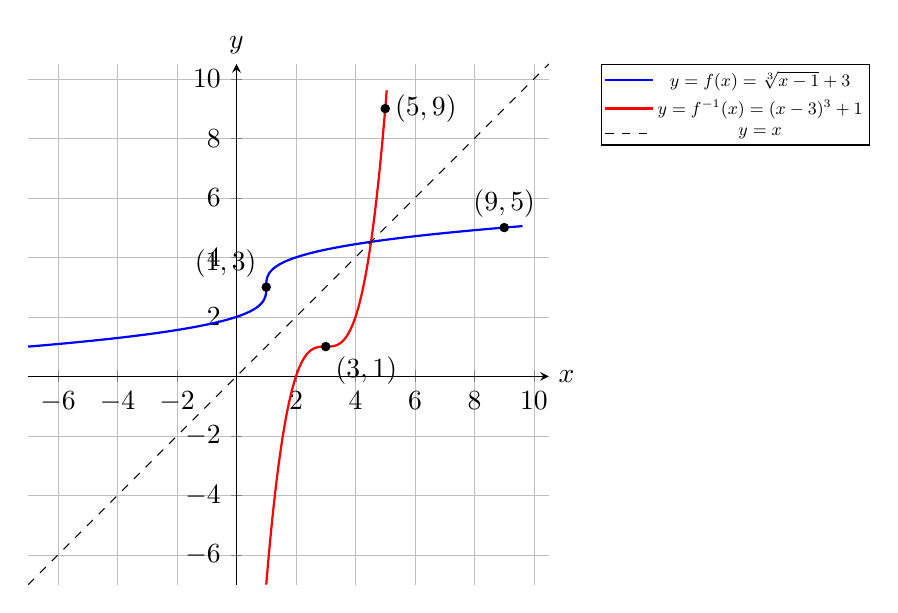
\begin{tikzpicture}
                    \begin{axis}[
        axis lines = middle,
        xlabel = $x$,
        ylabel = {$y$},
        grid=both,
        grid style={line width=.1pt, draw=gray!10},
        major grid style={line width=.2pt,draw=gray!50},
        x label style={anchor=west}, % label x ke kanan
        y label style={anchor=south}, % label y ke atas
        samples=200,
        legend style={
                at={(1.1,1)},
                anchor=north west,
                font=\small,         % mengecilkan ukuran font
                row sep=1pt,         % jarak antar baris legend
                inner sep=1pt,       % margin dalam kotak legend
                nodes={scale=0.7}    % skalakan isi legend
            },
        xtick={-6,-4,...,10},
        ytick={-6,-4,...,10},
        xmin=-7, xmax=10.5,
        ymin=-7, ymax=10.5,
        axis equal image,
        width=9.5cm
    ]
\addplot[domain=-2:2.05, color=blue, thick, variable=\t] ({(\t)*(\t)*(\t)+1},{\t+3});
\addlegendentry{$y=f(x)=\sqrt[3]{x-1}+3$}
\addplot[domain=-2:2.05, color=red, thick, variable=\t] ({\t+3},{(\t)*(\t)*(\t)+1});
\addlegendentry{$y=f^{-1}(x)=(x-3)^3+1$}
\addplot[domain=-7:10.5, color=black, dashed, samples=2] {x};
\addlegendentry{$y=x$}
\draw[fill=black] (1,3) circle (1.5pt) node[above left] {$(1,3)$};
\draw[fill=black] (9,5) circle (1.5pt) node[above] {$(9,5)$};
\draw[fill=black] (3,1) circle (1.5pt) node[below right] {$(3,1)$};
\draw[fill=black] (5,9) circle (1.5pt) node[right] {$(5,9)$};
\end{axis}
                \end{tikzpicture}
            \end{center}
        \end{enumerate}
    }
    \end{jawab}

    \item Hitunglah $\displaystyle\lim_{x\to-\infty}\frac{\sqrt{4x^2+3}}{2-x}$.
    \begin{jawab}[limit di tak hingga, bentuk akar, nilai mutlak]{~\\
        Diperhatikan bahwa jika $x\to-\infty$, pembilang dan penyebut sama-sama menuju tak hingga, sehingga diperoleh bentuk tak tentu $\frac{\infty}{\infty}$. Untuk menyelesaikannya, keluarkan $x^2$ dari dalam akar dengan mengingat bahwa $\colorlet{oldcolor}{.}
        \color{blue}
        \setlength{\fboxrule}{1pt} \boxed{\color{oldcolor}\sqrt{x^2}=|x|}\color{oldcolor}$, dan karena $x\to-\infty$ (yaitu $x<0$), maka $\colorlet{oldcolor}{.}
        \color{blue}
        \setlength{\fboxrule}{1pt} \boxed{\color{oldcolor}|x|=-x}\color{oldcolor}$. Diperoleh
        \begin{align*}
            \sqrt{4x^2+3} = \sqrt{x^2\left(4+\frac{3}{x^2}\right)} = |x|\sqrt{4+\frac{3}{x^2}} = -x\sqrt{4+\frac{3}{x^2}}.
        \end{align*}
        Dengan demikian,
        \begin{align*}
            \lim_{x\to-\infty}\frac{\sqrt{4x^2+3}}{2-x} &= \lim_{x\to-\infty}\frac{-x\sqrt{4+\frac{3}{x^2}}}{-x\left(1-\frac{2}{x}\right)}\\
            &= \lim_{x\to-\infty}\frac{\sqrt{4+\frac{3}{x^2}}}{1-\frac{2}{x}}\\
            &= \frac{\sqrt{4+0}}{1-0}\\
            &= \colorlet{oldcolor}{.}
        \color{red}
        \setlength{\fboxrule}{1pt} \boxed{\color{oldcolor}2}\color{oldcolor}.
        \end{align*}
    }
    \end{jawab}

    \item Dapatkan persamaan garis singgung kurva $xy^2+2y-\sqrt{x}=2$ di titik $(1,1)$.
    \begin{jawab}[diferensiasi implisit, aturan perkalian, persamaan garis singgung]{~\\
        Terlebih dahulu dicek bahwa titik $(1,1)$ terletak pada kurva, yaitu $1(1)^2+2(1)-\sqrt{1}=1+2-1=2$. Selanjutnya, kita turunkan kedua ruas terhadap $x$, dengan mengingat bahwa $y$ adalah fungsi dari $x$. Dengan aturan perkalian dan aturan rantai, diperoleh
        \begin{align*}
            \colorlet{oldcolor}{.}
        \color{blue}
        \setlength{\fboxrule}{1pt} \boxed{\color{oldcolor}\frac{d}{dx}(xy^2) = y^2 + 2xy\frac{dy}{dx}}\color{oldcolor}.
        \end{align*}
        Dengan demikian, diperoleh
        \begin{align*}
            y^2 + 2xy\frac{dy}{dx} + 2\frac{dy}{dx} - \frac{1}{2\sqrt{x}} &= 0\\
            (2xy + 2)\frac{dy}{dx} &= \frac{1}{2\sqrt{x}} - y^2\\
            \frac{dy}{dx} &= \colorlet{oldcolor}{.}
        \color{blue}
        \setlength{\fboxrule}{1pt} \boxed{\color{oldcolor}\frac{\frac{1}{2\sqrt{x}} - y^2}{2xy + 2}}\color{oldcolor}.
        \end{align*}
        Selanjutnya, substitusi titik $(1,1)$ ke dalam turunan:
        \begin{align*}
            m = \frac{dy}{dx}\bigg|_{(1,1)} = \frac{\frac{1}{2} - 1}{2(1)(1) + 2} = \frac{-\frac{1}{2}}{4} = \colorlet{oldcolor}{.}
        \color{blue}
        \setlength{\fboxrule}{1pt} \boxed{\color{oldcolor}-\frac{1}{8}}\color{oldcolor}.
        \end{align*}
        Dengan menggunakan persamaan garis $y - y_1 = m(x - x_1)$, di mana $(x_1,y_1)=(1,1)$, diperoleh
        \begin{align*}
            y - 1 &= -\frac{1}{8}(x - 1)\\
            y &= -\frac{1}{8}x + \frac{9}{8}.
        \end{align*}
        Jadi persamaan garis singgung di titik $(1,1)$ adalah $\colorlet{oldcolor}{.}
        \color{red}
        \setlength{\fboxrule}{1pt} \boxed{\color{oldcolor}y = -\frac{1}{8}x + \frac{9}{8}}\color{oldcolor}$ atau $x+8y=9$.
    }
    \end{jawab}
\end{enumerate}

\newpage

%%%%%%%%%%%%%%%%%%%%%%%%%%%%%%%%%%%%%%%%%%%%%%%%%%%%%%%%%%%%%%%%%%%%%%%%%%%%%%
% Kal-10
\kopsoal{Kal-10}{49-50}{Teknologi Kedokteran}{Selasa, Kamis; 12.30-15.00}{8}
\begin{enumerate}
    \item Dapatkan himpunan penyelesaian dari $\dfrac{2}{x+1}<\dfrac{1}{3-x}$.
    \begin{jawab}[pertidaksamaan rasional, pecahan, garis bilangan, notasi interval]{~\\
        Untuk menyelesaikan pertidaksamaan rasional, pastikan ruas kanan sudah bernilai nol (jangan dikali silang, karena tanda penyebutnya belum diketahui). Dengan mengurangkan \(\frac{1}{3-x}\) dari kedua ruas, didapatkan
        \[
        \frac{2}{x+1} - \frac{1}{3-x} < 0
        \]
        Selanjutnya, dengan menyamakan penyebut dan menyederhanakan bentuknya, diperoleh
        \begin{align}
            \frac{2(3-x)-(x+1)}{(x+1)(3-x)} &< 0\nonumber\\
            \frac{6-2x-x-1}{(x+1)(3-x)} &< 0\nonumber \\
            \frac{5-3x}{(x+1)(3-x)} &< 0 \label{ineq:kal10}
        \end{align}
        Didapatkan pembuat nol dari faktor-faktornya adalah
        \begin{align*}
            5-3x = 0 \quad &\vee\quad  x+1 = 0 \quad\vee\quad 3-x=0\\
            \colorlet{oldcolor}{.}
        \color{blue}
        \setlength{\fboxrule}{1pt} \boxed{\color{oldcolor}x=\frac{5}{3}}\color{oldcolor} \quad &\vee\quad \colorlet{oldcolor}{.}
        \color{blue}
        \setlength{\fboxrule}{1pt} \boxed{\color{oldcolor}x=-1}\color{oldcolor} \quad\vee\quad \colorlet{oldcolor}{.}
        \color{blue}
        \setlength{\fboxrule}{1pt} \boxed{\color{oldcolor}x=3}\color{oldcolor}
        \end{align*}
        Selanjutnya, dibuat garis bilangan dan dilakukan uji titik pada ekspresi \eqref{ineq:kal10} sebagai berikut
        \begin{itemize}
            \item Untuk \(x < -1\), misalkan \(x = -2\):
            \[
            \frac{5-3(-2)}{(-2+1)(3-(-2))} = \frac{11}{(-1)(5)} = \frac{11}{-5} < 0
            \]
            \item Untuk \(-1 < x < \frac{5}{3}\), misalkan \(x = 0\):
            \[
            \frac{5-0}{(0+1)(3-0)} = \frac{5}{3} > 0
            \]
            \item Untuk \(\frac{5}{3} < x < 3\), misalkan \(x = 2\):
            \[
            \frac{5-6}{(2+1)(3-2)} = \frac{-1}{3} < 0
            \]
            \item Untuk \(x > 3\), misalkan \(x = 4\):
            \[
            \frac{5-12}{(4+1)(3-4)} = \frac{-7}{-5} > 0
            \]
        \end{itemize}
        \begin{center}
           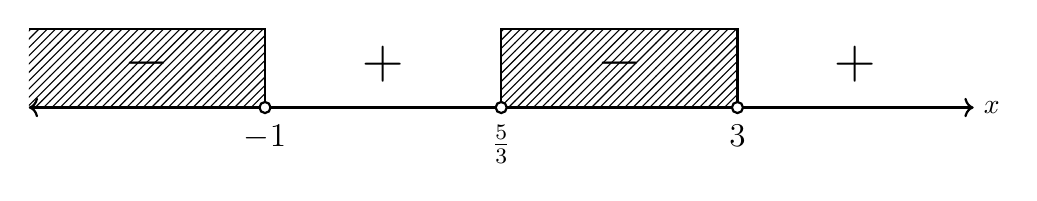
\begin{tikzpicture}
    \draw[thick,<->] (-6,0) -- (6,0) node[right] {$x$};
    \fill[pattern=north east lines] (-6,0) rectangle (-3,1);
    \fill[pattern=north east lines] (0,0) rectangle (3,1);
    \draw[thick] (-6,1) -- (-3,1) -- (-3,0);
    \draw[thick] (0,0) -- (0,1) -- (3,1) -- (3,0);
    \draw (-3,-0.1) node[below] {\large{$-1$}};
    \draw (0,-0.1) node[below] {\large{$\frac{5}{3}$}};
    \draw (3,-0.1) node[below] {\large{$3$}};
    \draw (-4.5,0.2) node[above] {\huge{$-$}};
    \draw (-1.5,0.2) node[above] {\huge{$+$}};
    \draw (1.5,0.2) node[above] {\huge{$-$}};
    \draw (4.5,0.2) node[above] {\huge{$+$}};
    \draw[fill=white, thick] (-3,0) circle (2pt);
    \draw[fill=white, thick] (0,0) circle (2pt);
    \draw[fill=white, thick] (3,0) circle (2pt);
\end{tikzpicture}
        \end{center}
        Karena yang diminta adalah nilai \(x\) yang membuat pertidaksamaan \eqref{ineq:kal10} kurang dari nol, diambil interval yang bertanda negatif tanpa pembuat nol. Jadi himpunan penyelesaiannya adalah
        \[
        \colorlet{oldcolor}{.}
        \color{red}
        \setlength{\fboxrule}{1pt} \boxed{\color{oldcolor}\left\{x\in\mathbb{R} : x<-1 \;\vee\; \frac{5}{3}<x<3\right\} = (-\infty,-1)\cup\left(\frac{5}{3},3\right)}\color{oldcolor}.
        \]
    }
    \end{jawab}

    \item Diberikan fungsi $f(x)=\sqrt{2-x}$ dan $g(x)=\dfrac{1}{\sqrt{16-x^2}}$.
    \begin{enumerate}
        \item Dapatkan domain $f$ dan $g$.
        \item Dapatkan $(g\circ f)(x)$ beserta domainnya.
    \end{enumerate}
    \begin{jawab}[domain fungsi, fungsi komposisi, domain fungsi komposisi]{
        \begin{enumerate}
            \item Diperhatikan bahwa $f(x)$ memuat akar kuadrat, sehingga syaratnya adalah $2-x\geq 0$, yaitu $x\leq 2$. Jadi
            \begin{align*}
                \colorlet{oldcolor}{.}
        \color{red}
        \setlength{\fboxrule}{1pt} \boxed{\color{oldcolor}D(f)=\{x\in\mathbb{R} : x\leq 2\}=(-\infty,2]}\color{oldcolor}.
            \end{align*}
            Selanjutnya, $g(x)$ memuat akar kuadrat di penyebut, sehingga ekspresi di dalam akar harus positif (tidak boleh nol), yaitu $16-x^2>0$ atau $(4-x)(4+x)>0$, yang dipenuhi oleh $-4<x<4$. Jadi
            \begin{align*}
                \colorlet{oldcolor}{.}
        \color{red}
        \setlength{\fboxrule}{1pt} \boxed{\color{oldcolor}D(g)=\{x\in\mathbb{R} : -4<x<4\}=(-4,4)}\color{oldcolor}.
            \end{align*}
            \item Diperhatikan bahwa
            \begin{align*}
                (g\circ f)(x) = g(f(x)) = \frac{1}{\sqrt{16-\left(\sqrt{2-x}\right)^2}} = \frac{1}{\sqrt{16-(2-x)}} = \colorlet{oldcolor}{.}
        \color{red}
        \setlength{\fboxrule}{1pt} \boxed{\color{oldcolor}\frac{1}{\sqrt{14+x}}}\color{oldcolor}.
            \end{align*}
            Domain dari fungsi komposisi $g\circ f$ adalah semua nilai $x$ pada domain $f$ sehingga nilai dari $f(x)$ berada pada domain $g$, yang dapat dirumuskan sebagai
            \begin{align*}
                \colorlet{oldcolor}{.}
        \color{blue}
        \setlength{\fboxrule}{1pt} \boxed{\color{oldcolor}D(g\circ f) = \{x \in D(f) : f(x) \in D(g)\} = \left\{x \leq 2 : -4<\sqrt{2-x}<4\right\}}\color{oldcolor}.
            \end{align*}
            Karena $\sqrt{2-x}\geq 0>-4$, syarat $\sqrt{2-x}>-4$ selalu berlaku. Selanjutnya, $\sqrt{2-x}<4$ jika dan hanya jika $2-x<16$, yaitu $x>-14$. Dengan menggabungkan syarat $x\leq 2$, didapatkan
            \begin{align*}
                \colorlet{oldcolor}{.}
        \color{red}
        \setlength{\fboxrule}{1pt} \boxed{\color{oldcolor}D(g\circ f) = \{x\in\mathbb{R} : -14<x\leq 2\} = (-14,2]}\color{oldcolor}.
            \end{align*}
            \textit{Catatan:} meskipun bentuk akhir $\frac{1}{\sqrt{14+x}}$ terdefinisi untuk $x>2$, nilai-nilai tersebut tidak termasuk domain karena $f(x)$ tidak terdefinisi di sana.
        \end{enumerate}
    }
    \end{jawab}

    \item Diberikan suatu fungsi $f(x)=1-\sqrt{6x-x^2}$ dengan domain $f$ adalah $[0,a]$.
    \begin{enumerate}
        \item Dapatkan nilai terbesar $a$ sehingga $f^{-1}(x)$ ada.
        \item Tentukan $f^{-1}(x)$.
        \item Gambarkan sketsa kurva $f(x)$ dan $f^{-1}(x)$ dalam satu bidang koordinat.
    \end{enumerate}
    \begin{jawab}[melengkapkan kuadrat, setengah lingkaran, fungsi satu-satu, fungsi invers]{
        \begin{enumerate}
            \item Dengan melengkapkan kuadrat, diperoleh $6x-x^2=9-(x^2-6x+9)=\colorlet{oldcolor}{.}
        \color{blue}
        \setlength{\fboxrule}{1pt} \boxed{\color{oldcolor}9-(x-3)^2}\color{oldcolor}$, sehingga $f(x)=1-\sqrt{9-(x-3)^2}$ yang terdefinisi untuk $0\leq x\leq 6$. Jika $y=f(x)$, maka $1-y=\sqrt{9-(x-3)^2}\geq 0$ dan
            \begin{align*}
                (1-y)^2 = 9-(x-3)^2 \iff \colorlet{oldcolor}{.}
        \color{blue}
        \setlength{\fboxrule}{1pt} \boxed{\color{oldcolor}(x-3)^2+(y-1)^2=9}\color{oldcolor},\quad y\leq 1,
            \end{align*}
            sehingga grafik $f$ adalah setengah lingkaran bagian bawah dengan pusat $(3,1)$ dan jari-jari $3$. Grafik ini turun pada $[0,3]$ dan naik pada $[3,6]$. Agar $f$ satu-satu pada $[0,a]$, domain tidak boleh melewati titik terendah $x=3$, sehingga haruslah $a\leq 3$. Jadi nilai terbesar $a$ adalah $\colorlet{oldcolor}{.}
        \color{red}
        \setlength{\fboxrule}{1pt} \boxed{\color{oldcolor}a=3}\color{oldcolor}$.
            \item Misalkan $y=f(x)$ dengan $x\in[0,3]$, kemudian selesaikan sehingga terbentuk $x$ dalam fungsi $y$. Diperoleh
            \begin{align*}
                y &= 1-\sqrt{9-(x-3)^2}\\
                \sqrt{9-(x-3)^2} &= 1-y\\
                9-(x-3)^2 &= (1-y)^2\\
                (x-3)^2 &= 9-(y-1)^2\\
                x-3 &= -\sqrt{9-(y-1)^2} \quad (\text{karena } x\leq 3)\\
                x &= 3-\sqrt{9-(y-1)^2}.
            \end{align*}
            Dari sini didapatkan $x = f^{-1}(y) = 3-\sqrt{9-(y-1)^2}$. Dengan mengganti $y$ dengan $x$, diperoleh
            \begin{align*}
                \colorlet{oldcolor}{.}
        \color{red}
        \setlength{\fboxrule}{1pt} \boxed{\color{oldcolor}f^{-1}(x) = 3-\sqrt{9-(x-1)^2} = 3-\sqrt{8+2x-x^2}}\color{oldcolor}.
            \end{align*}
            Pada domain $[0,3]$, fungsi $f$ turun dari $f(0)=1$ sampai $f(3)=1-3=-2$, sehingga $D(f^{-1})=R(f)=[-2,1]$ dan $R(f^{-1})=D(f)=[0,3]$.
            \item Grafik $f$ adalah seperempat lingkaran berpusat di $(3,1)$ dari titik $(0,1)$ ke $(3,-2)$. Grafik $f^{-1}$ merupakan pencerminan grafik $f$ terhadap garis $y=x$, yaitu seperempat lingkaran $(x-1)^2+(y-3)^2=9$ yang berpusat di $(1,3)$, dari titik $(1,0)$ ke $(-2,3)$. Sketsa grafiknya adalah sebagai berikut.
            \begin{center}
                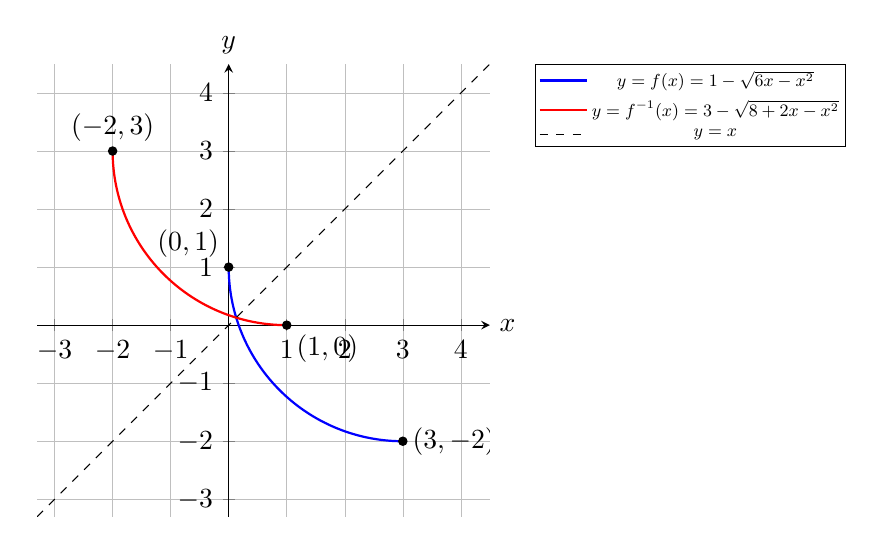
\begin{tikzpicture}
                    \begin{axis}[
        axis lines = middle,
        xlabel = $x$,
        ylabel = {$y$},
        grid=both,
        grid style={line width=.1pt, draw=gray!10},
        major grid style={line width=.2pt,draw=gray!50},
        x label style={anchor=west}, % label x ke kanan
        y label style={anchor=south}, % label y ke atas
        samples=200,
        legend style={
                at={(1.1,1)},
                anchor=north west,
                font=\small,         % mengecilkan ukuran font
                row sep=1pt,         % jarak antar baris legend
                inner sep=1pt,       % margin dalam kotak legend
                nodes={scale=0.7}    % skalakan isi legend
            },
        xtick={-3,-2,...,4},
        ytick={-3,-2,...,4},
        xmin=-3.3, xmax=4.5,
        ymin=-3.3, ymax=4.5,
        axis equal image,
        width=8.5cm
    ]
\addplot[domain=180:270, color=blue, thick] ({3+3*cos(x)}, {1+3*sin(x)});
\addlegendentry{$y=f(x)=1-\sqrt{6x-x^2}$}
\addplot[domain=180:270, color=red, thick] ({1+3*sin(x)}, {3+3*cos(x)});
\addlegendentry{$y=f^{-1}(x)=3-\sqrt{8+2x-x^2}$}
\addplot[domain=-3.3:4.5, color=black, dashed, samples=2] {x};
\addlegendentry{$y=x$}
\draw[fill=black] (0,1) circle (1.5pt) node[above left] {$(0,1)$};
\draw[fill=black] (3,-2) circle (1.5pt) node[right] {$(3,-2)$};
\draw[fill=black] (1,0) circle (1.5pt) node[below right] {$(1,0)$};
\draw[fill=black] (-2,3) circle (1.5pt) node[above] {$(-2,3)$};
\end{axis}
                \end{tikzpicture}
            \end{center}
        \end{enumerate}
    }
    \end{jawab}

    \item Tunjukkan bahwa $f(x)=\begin{cases}
        x^2+1, & x\leq 1\\
        4x-2, & x>1
    \end{cases}$ adalah fungsi kontinu tetapi tidak dapat diturunkan di $x=1$.
    \begin{jawab}[fungsi kontinu, limit sepihak, turunan sepihak]{~\\
        Ingat kembali syarat fungsi kontinu di suatu titik \(x = a\) adalah
        \begin{enumerate}
            \item \(f(a)\) terdefinisi
            \item \(\displaystyle \lim_{x \to a} f(x)\) ada, yaitu $\displaystyle \lim_{x \to a^-} f(x) = \lim_{x \to a^+} f(x)$
            \item \(\displaystyle\lim_{x \to a} f(x) = f(a)\)
        \end{enumerate}
        Diperhatikan bahwa untuk $x=1$, $\colorlet{oldcolor}{.}
        \color{blue}
        \setlength{\fboxrule}{1pt} \boxed{\color{oldcolor}f(1) = 1^2+1 = 2~\text{terdefinisi}}\color{oldcolor}$. Selanjutnya, limit kiri dan limit kanannya adalah
        \begin{align*}
            \lim_{x\to 1^-} f(x) = \lim_{x\to 1^-} (x^2+1) = 2 \quad\text{dan}\quad \lim_{x\to 1^+} f(x) = \lim_{x\to 1^+} (4x-2) = 2,
        \end{align*}
        sehingga $\colorlet{oldcolor}{.}
        \color{blue}
        \setlength{\fboxrule}{1pt} \boxed{\color{oldcolor}\lim_{x\to 1} f(x) = 2 = f(1)}\color{oldcolor}$. Jadi $\colorlet{oldcolor}{.}
        \color{red}
        \setlength{\fboxrule}{1pt} \boxed{\color{oldcolor}f \text{ kontinu di } x=1}\color{oldcolor}$.\\
        Selanjutnya, ingat bahwa $f$ dapat diturunkan di $x=a$ jika limit $\displaystyle f'(a)=\lim_{h\to 0}\frac{f(a+h)-f(a)}{h}$ ada, yaitu turunan kiri sama dengan turunan kanan. Untuk turunan kiri ($h<0$, sehingga $1+h<1$), diperoleh
        \begin{align*}
            f'_-(1) = \lim_{h\to 0^-}\frac{f(1+h)-f(1)}{h} = \lim_{h\to 0^-}\frac{(1+h)^2+1-2}{h} = \lim_{h\to 0^-}\frac{2h+h^2}{h} = \lim_{h\to 0^-}(2+h) = \colorlet{oldcolor}{.}
        \color{blue}
        \setlength{\fboxrule}{1pt} \boxed{\color{oldcolor}2}\color{oldcolor}.
        \end{align*}
        Untuk turunan kanan ($h>0$, sehingga $1+h>1$), diperoleh
        \begin{align*}
            f'_+(1) = \lim_{h\to 0^+}\frac{f(1+h)-f(1)}{h} = \lim_{h\to 0^+}\frac{4(1+h)-2-2}{h} = \lim_{h\to 0^+}\frac{4h}{h} = \colorlet{oldcolor}{.}
        \color{blue}
        \setlength{\fboxrule}{1pt} \boxed{\color{oldcolor}4}\color{oldcolor}.
        \end{align*}
        Karena $f'_-(1)=2\neq 4=f'_+(1)$, maka $f'(1)$ tidak ada. Jadi terbukti bahwa
        \[\colorlet{oldcolor}{.}
        \color{red}
        \setlength{\fboxrule}{1pt} \boxed{\color{oldcolor}f \text{ kontinu tetapi tidak dapat diturunkan di } x=1}\color{oldcolor}.\]
        Secara grafik, di titik $(1,2)$ grafik $f$ membentuk ``sudut'' (tidak mulus).
    }
    \end{jawab}

    \item Diketahui kurva $xy^2+y^3=2x+8$.
    \begin{enumerate}
        \item Tentukan $\dfrac{dy}{dx}$.
        \item Dapatkan persamaan garis singgung kurva tersebut di titik $(0,2)$.
    \end{enumerate}
    \begin{jawab}[turunan implisit, aturan perkalian, persamaan garis singgung]{
        \begin{enumerate}
            \item Kita turunkan kedua ruas persamaan $xy^2+y^3=2x+8$ terhadap $x$, dengan mengingat bahwa $y$ adalah fungsi dari $x$ (yaitu $y=y(x)$). Dengan aturan perkalian, $\colorlet{oldcolor}{.}
        \color{blue}
        \setlength{\fboxrule}{1pt} \boxed{\color{oldcolor}\frac{d}{dx}(xy^2) = y^2 + 2xy\frac{dy}{dx}}\color{oldcolor}$, dan dengan aturan rantai, $\colorlet{oldcolor}{.}
        \color{blue}
        \setlength{\fboxrule}{1pt} \boxed{\color{oldcolor}\frac{d}{dx}(y^3) = 3y^2\frac{dy}{dx}}\color{oldcolor}$. Diperoleh
            \begin{align*}
                y^2 + 2xy\frac{dy}{dx} + 3y^2\frac{dy}{dx} &= 2\\
                (2xy + 3y^2)\frac{dy}{dx} &= 2 - y^2\\
                \frac{dy}{dx} &= \frac{2 - y^2}{2xy + 3y^2}.
            \end{align*}
            Jadi diperoleh $\colorlet{oldcolor}{.}
        \color{red}
        \setlength{\fboxrule}{1pt} \boxed{\color{oldcolor}\frac{dy}{dx} = \frac{2 - y^2}{2xy + 3y^2}}\color{oldcolor}$.
            \item Terlebih dahulu dicek bahwa titik $(0,2)$ terletak pada kurva, yaitu $0(2)^2+2^3=8=2(0)+8$. Untuk mendapatkan gradien garis singgung di titik $(0,2)$, substitusi $x=0$ dan $y=2$ ke dalam turunan yang telah diperoleh:
            \begin{align*}
                m=\left.\frac{dy}{dx}\right|_{(0,2)} = \frac{2 - 2^2}{2(0)(2) + 3(2)^2}= \frac{-2}{12}= \colorlet{oldcolor}{.}
        \color{blue}
        \setlength{\fboxrule}{1pt} \boxed{\color{oldcolor}-\frac{1}{6}}\color{oldcolor}.
            \end{align*}
            Dengan menggunakan persamaan garis $y - y_1 = m(x - x_1)$, di mana $(x_1,y_1)=(0,2)$ dan $m=-\frac{1}{6}$, diperoleh:
            \begin{align*}
                y - 2 &= -\frac{1}{6}(x - 0)\\
                y &= -\frac{1}{6}x + 2.
            \end{align*}
            Jadi persamaan garis singgung di titik $(0,2)$ adalah $\colorlet{oldcolor}{.}
        \color{red}
        \setlength{\fboxrule}{1pt} \boxed{\color{oldcolor}y = -\frac{1}{6}x + 2}\color{oldcolor}$ atau $x+6y=12$.
        \end{enumerate}
    }
    \end{jawab}
\end{enumerate}

\newpage

%%%%%%%%%%%%%%%%%%%%%%%%%%%%%%%%%%%%%%%%%%%%%%%%%%%%%%%%%%%%%%%%%%%%%%%%%%%%%%
% Kal-iup-3
\kopsoaliup{Kal-iup-3}{63, 64, 70}{Civil, Geomatics, Geophysical Engineering, Naval Architecture (JD)}{Tuesday, Thursday; 15.30-17.10}{9}
\begin{enumerate}
    \item Find the solution of the following inequality
    \begin{align*}
        \frac{x^2-5x+4}{x^2-x-6}\geq 0.
    \end{align*}
    \begin{jawab}[pertidaksamaan rasional, faktorisasi, garis bilangan, notasi interval]{~\\
    Karena ruas kanan pertidaksamaan sudah bernilai nol, maka kita bisa langsung memfaktorkan pembilang dan penyebut di ruas kiri. Diperoleh
    \begin{align*}
        \frac{x^2-5x+4}{x^2-x-6} = \frac{(x-1)(x-4)}{(x-3)(x+2)} \geq 0.
    \end{align*}
    Selanjutnya, kita tentukan pembuat nol dari faktor-faktor tersebut, yaitu
    \begin{align*}
        x-1 = 0 \quad &\vee\quad x-4 = 0 \quad \vee\quad x-3 = 0 \quad \vee\quad x+2 = 0\\
        \colorlet{oldcolor}{.}
        \color{blue}
        \setlength{\fboxrule}{1pt} \boxed{\color{oldcolor}x=1}\color{oldcolor} \quad &\vee\quad \colorlet{oldcolor}{.}
        \color{blue}
        \setlength{\fboxrule}{1pt} \boxed{\color{oldcolor}x=4}\color{oldcolor} \quad \vee\quad \colorlet{oldcolor}{.}
        \color{blue}
        \setlength{\fboxrule}{1pt} \boxed{\color{oldcolor}x=3}\color{oldcolor} \quad \vee\quad \colorlet{oldcolor}{.}
        \color{blue}
        \setlength{\fboxrule}{1pt} \boxed{\color{oldcolor}x=-2}\color{oldcolor}
    \end{align*}
    Selanjutnya, kita buat garis bilangan dan lakukan uji titik pada ekspresi \(\frac{(x-1)(x-4)}{(x-3)(x+2)}\) sebagai berikut
    \begin{itemize}
        \item Untuk \(x < -2\), misalkan \(x = -3\):
        \[
        \frac{(-3-1)(-3-4)}{(-3-3)(-3+2)} = \frac{(-4)(-7)}{(-6)(-1)} = \frac{28}{6} > 0
        \]
        \item Untuk \(-2 < x < 1\), misalkan \(x = 0\):
        \[
        \frac{(0-1)(0-4)}{(0-3)(0+2)} = \frac{(-1)(-4)}{(-3)(2)} = \frac{4}{-6} < 0
        \]
        \item Untuk \(1 < x < 3\), misalkan \(x = 2\):
        \[
        \frac{(2-1)(2-4)}{(2-3)(2+2)} = \frac{(1)(-2)}{(-1)(4)} = \frac{2}{4} > 0
        \]
        \item Untuk \(3 < x < 4\), misalkan \(x = 3.5\):
        \[
        \frac{(3.5-1)(3.5-4)}{(3.5-3)(3.5+2)} = \frac{(2.5)(-0.5)}{(0.5)(5.5)} = \frac{-1.25}{2.75} < 0
        \]
        \item Untuk \(x > 4\), misalkan \(x = 5\):
        \[
        \frac{(5-1)(5-4)}{(5-3)(5+2)} = \frac{(4)(1)}{(2)(7)} = \frac{4}{14} > 0
        \]
    \end{itemize}
    \begin{center}
        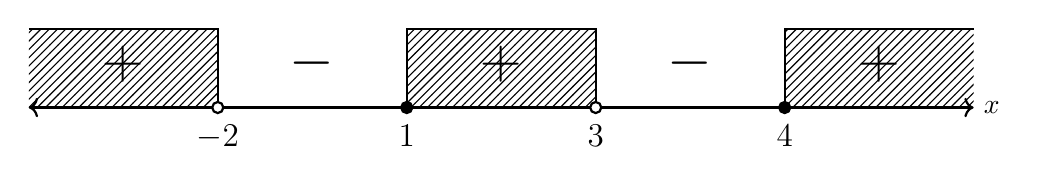
\begin{tikzpicture}
    \draw[thick,<->] (-6,0) -- (6,0) node[right] {$x$};
    \fill[pattern=north east lines] (-6,0) rectangle (-3.6,1);
    \fill[pattern=north east lines] (-1.2,0) rectangle (1.2,1);
    \fill[pattern=north east lines] (3.6,0) rectangle (6,1);
    \draw[thick] (-6,1) -- (-3.6,1) -- (-3.6,0);
    \draw[thick] (-1.2,0) -- (-1.2,1) -- (1.2,1) -- (1.2,0);
    \draw[thick] (3.6,0) -- (3.6,1) -- (6,1);
    \draw (-3.6,-0.1) node[below] {\large{$-2$}};
    \draw (-1.2,-0.1) node[below] {\large{$1$}};
    \draw (1.2,-0.1) node[below] {\large{$3$}};
    \draw (3.6,-0.1) node[below] {\large{$4$}};
    \draw (-4.8,0.2) node[above] {\huge{$+$}};
    \draw (-2.4,0.2) node[above] {\huge{$-$}};
    \draw (0,0.2) node[above] {\huge{$+$}};
    \draw (2.4,0.2) node[above] {\huge{$-$}};
    \draw (4.8,0.2) node[above] {\huge{$+$}};
    \draw[fill=white, thick] (-3.6,0) circle (2pt);
    \draw[fill=black, thick] (-1.2,0) circle (2pt);
    \draw[fill=white, thick] (1.2,0) circle (2pt);
    \draw[fill=black, thick] (3.6,0) circle (2pt);
        \end{tikzpicture}
    \end{center}
    Karena yang diminta adalah nilai yang lebih dari atau sama dengan nol, diambil interval yang bertanda positif beserta pembuat nol dari pembilang ($x=1$ dan $x=4$). Pembuat nol dari penyebut ($x=-2$ dan $x=3$) tidak diikutkan karena membuat ekspresi tidak terdefinisi. Jadi solusi dari pertidaksamaan tersebut adalah \(x < -2\) atau \(1 \leq x < 3\) atau \(x \geq 4\). Dalam notasi interval, solusi tersebut dapat ditulis sebagai $\colorlet{oldcolor}{.}
        \color{red}
        \setlength{\fboxrule}{1pt} \boxed{\color{oldcolor}(-\infty, -2) \cup [1, 3) \cup [4, \infty)}\color{oldcolor}$.
    }
    \end{jawab}

    \item \begin{enumerate}
        \item Find the gradient of the line $\ell$ which goes through $(0,0)$ and $(1,3)$.
        \item If line $\ell$ is perpendicular with the line that tangent with a circle centered at $(0,0)$ and radius $\sqrt{10}$, at $(1,3)$, then find the aforementioned tangent line equation and sketch the graph.
    \end{enumerate}
    \begin{jawab}[kemiringan garis, garis tegak lurus, garis singgung lingkaran]{
        \begin{enumerate}
            \item Kemiringan garis yang melalui dua titik $(x_1,y_1)$ dan $(x_2,y_2)$ adalah
            \begin{align*}
                m = \frac{y_2 - y_1}{x_2 - x_1}.
            \end{align*}
            Dengan substitusi $(x_1,y_1)=(0,0)$ dan $(x_2,y_2)=(1,3)$, diperoleh
            \begin{align*}
                m_\ell = \frac{3 - 0}{1 - 0} = 3.
            \end{align*}
            Jadi kemiringan garis $\ell$ adalah $\colorlet{oldcolor}{.}
        \color{red}
        \setlength{\fboxrule}{1pt} \boxed{\color{oldcolor}m_\ell = 3}\color{oldcolor}$.
            \item Persamaan lingkaran yang berpusat di $(0,0)$ dan berjari-jari $\sqrt{10}$ adalah $x^2 + y^2 = 10$. Diperhatikan bahwa titik $(1,3)$ terletak pada lingkaran, karena $1^2 + 3^2 = 1 + 9 = 10$. \\
            Ingat kembali bahwa dua garis dengan gradien $m_1$ dan $m_2$ saling tegak lurus jika $\colorlet{oldcolor}{.}
        \color{blue}
        \setlength{\fboxrule}{1pt} \boxed{\color{oldcolor}m_1\cdot m_2=-1}\color{oldcolor}$. Karena garis singgung tegak lurus dengan garis $\ell$, maka gradien garis singgung $m_s$ memenuhi
            \begin{align*}
                m_\ell \cdot m_s = -1 \implies 3\cdot m_s = -1 \implies \colorlet{oldcolor}{.}
        \color{blue}
        \setlength{\fboxrule}{1pt} \boxed{\color{oldcolor}m_s = -\frac{1}{3}}\color{oldcolor}.
            \end{align*}
            Garis singgung melalui titik $(1,3)$ dengan gradien $-\frac{1}{3}$, sehingga dengan rumus $y - y_1 = m(x - x_1)$ diperoleh
            \begin{align*}
                y - 3 &= -\frac{1}{3}(x - 1)\\
                y &= -\frac{1}{3}x + \frac{1}{3} + 3\\
                y &= -\frac{1}{3}x + \frac{10}{3}.
            \end{align*}
            Jadi persamaan garis singgung lingkaran tersebut adalah $\colorlet{oldcolor}{.}
        \color{red}
        \setlength{\fboxrule}{1pt} \boxed{\color{oldcolor}y = -\frac{1}{3}x + \frac{10}{3}}\color{oldcolor}$ atau $x+3y=10$. Sketsa grafiknya adalah sebagai berikut:
            \begin{center}
                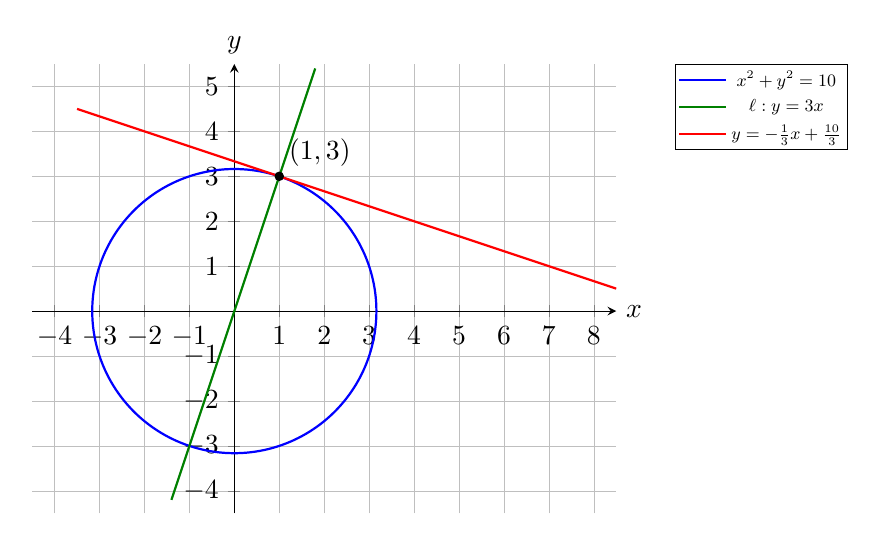
\begin{tikzpicture}
                    \begin{axis}[
        axis lines = middle,
        xlabel = $x$,
        ylabel = {$y$},
        grid=both,
        grid style={line width=.1pt, draw=gray!10},
        major grid style={line width=.2pt,draw=gray!50},
        x label style={anchor=west}, % label x ke kanan
        y label style={anchor=south}, % label y ke atas
        samples=200,
        legend style={
                at={(1.1,1)},
                anchor=north west,
                font=\small,         % mengecilkan ukuran font
                row sep=1pt,         % jarak antar baris legend
                inner sep=1pt,       % margin dalam kotak legend
                nodes={scale=0.7}    % skalakan isi legend
            },
        xtick={-4,-3,...,8},
        ytick={-4,-3,...,5},
        xmin=-4.5, xmax=8.5,
        ymin=-4.5, ymax=5.5,
        axis equal image,
        width=9cm
    ]
\addplot[domain=0:360, color=blue, thick] ({sqrt(10)*cos(x)}, {sqrt(10)*sin(x)});
\addlegendentry{$x^2+y^2=10$}
\addplot[domain=-1.4:1.8, color=green!50!black, thick, samples=2] {3*x};
\addlegendentry{$\ell: y=3x$}
\addplot[domain=-3.5:8.5, color=red, thick, samples=2] {-x/3+10/3};
\addlegendentry{$y=-\frac{1}{3}x+\frac{10}{3}$}
\draw[fill=black] (1,3) circle (1.5pt) node[above right] {$(1,3)$};
\end{axis}
                \end{tikzpicture}
            \end{center}
        \end{enumerate}
    }
    \end{jawab}

    \item Given $f(x)=x^3-1$.
    \begin{enumerate}
        \item Find $f^{-1}(x)$ and its domain.
        \item Sketch the graph of $f(x)$ and $f^{-1}(x)$ in the same coordinate plane.
    \end{enumerate}
    \begin{jawab}[fungsi invers, domain dan range, sketsa grafik fungsi invers]{
        \begin{enumerate}
            \item Fungsi $f(x)=x^3-1$ selalu naik, sehingga satu-satu dan mempunyai invers. Untuk mendapatkan fungsi invers dari $f(x)$, kita misalkan $y=f(x)$, kemudian selesaikan sehingga terbentuk $x$ dalam fungsi $y$. Diperoleh
            \begin{align*}
                y &= x^3-1\\
                x^3 &= y+1\\
                x &= \sqrt[3]{y+1}.
            \end{align*}
            Dari sini didapatkan $x = f^{-1}(y) = \sqrt[3]{y+1}$. Dengan mengganti $y$ dengan $x$, diperoleh $f^{-1}(x) = \sqrt[3]{x+1}$.\\
            Karena $f$ adalah fungsi polinomial berderajat tiga, maka $D(f)=\mathbb{R}$ dan $R(f)=\mathbb{R}$. Domain dari fungsi invers adalah range dari fungsi asli, yaitu $\colorlet{oldcolor}{.}
        \color{blue}
        \setlength{\fboxrule}{1pt} \boxed{\color{oldcolor}D(f^{-1}) = R(f) = \mathbb{R}}\color{oldcolor}$ (sesuai dengan akar pangkat tiga yang terdefinisi untuk setiap bilangan real). Jadi
            \begin{align*}
                \colorlet{oldcolor}{.}
        \color{red}
        \setlength{\fboxrule}{1pt} \boxed{\color{oldcolor}f^{-1}(x) = \sqrt[3]{x+1},\quad D(f^{-1})=\mathbb{R}}\color{oldcolor}.
            \end{align*}
            \item Grafik $f$ adalah grafik $y=x^3$ yang digeser $1$ satuan ke bawah, dengan titik belok $(0,-1)$. Grafik $f^{-1}$ merupakan pencerminan grafik $f$ terhadap garis $y=x$, dengan titik belok $(-1,0)$. Sebagai bantuan, grafik $f$ melalui titik $(-1,-2)$, $(0,-1)$, $(1,0)$, dan $(2,7)$, sehingga grafik $f^{-1}$ melalui titik $(-2,-1)$, $(-1,0)$, $(0,1)$, dan $(7,2)$. Sketsa grafiknya adalah sebagai berikut.
            \begin{center}
                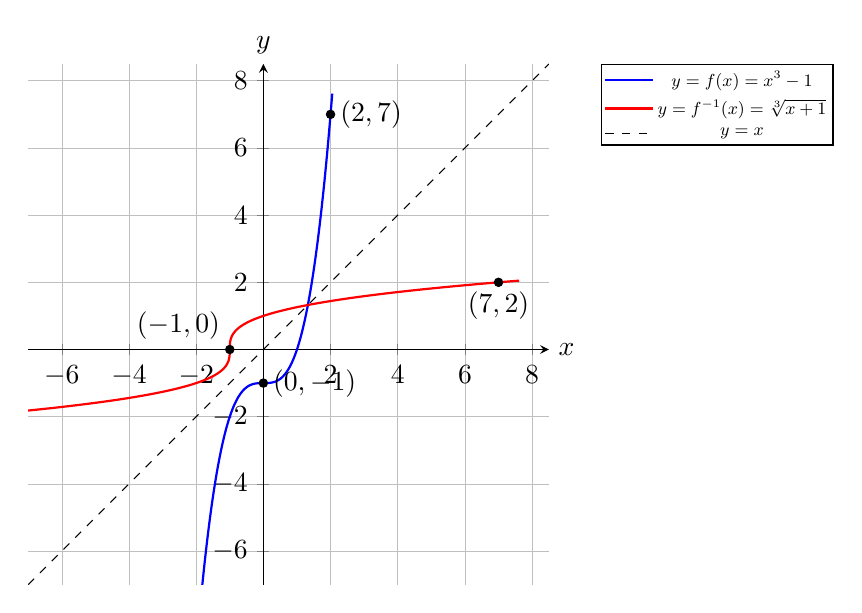
\begin{tikzpicture}
                    \begin{axis}[
        axis lines = middle,
        xlabel = $x$,
        ylabel = {$y$},
        grid=both,
        grid style={line width=.1pt, draw=gray!10},
        major grid style={line width=.2pt,draw=gray!50},
        x label style={anchor=west}, % label x ke kanan
        y label style={anchor=south}, % label y ke atas
        samples=200,
        legend style={
                at={(1.1,1)},
                anchor=north west,
                font=\small,         % mengecilkan ukuran font
                row sep=1pt,         % jarak antar baris legend
                inner sep=1pt,       % margin dalam kotak legend
                nodes={scale=0.7}    % skalakan isi legend
            },
        xtick={-6,-4,...,8},
        ytick={-6,-4,...,8},
        xmin=-7, xmax=8.5,
        ymin=-7, ymax=8.5,
        axis equal image,
        width=9.5cm
    ]
\addplot[domain=-1.85:2.05, color=blue, thick, variable=\t] ({\t},{(\t)*(\t)*(\t)-1});
\addlegendentry{$y=f(x)=x^3-1$}
\addplot[domain=-1.85:2.05, color=red, thick, variable=\t] ({(\t)*(\t)*(\t)-1},{\t});
\addlegendentry{$y=f^{-1}(x)=\sqrt[3]{x+1}$}
\addplot[domain=-7:8.5, color=black, dashed, samples=2] {x};
\addlegendentry{$y=x$}
\draw[fill=black] (0,-1) circle (1.5pt) node[right] {$(0,-1)$};
\draw[fill=black] (2,7) circle (1.5pt) node[right] {$(2,7)$};
\draw[fill=black] (-1,0) circle (1.5pt) node[above left] {$(-1,0)$};
\draw[fill=black] (7,2) circle (1.5pt) node[below] {$(7,2)$};
\end{axis}
                \end{tikzpicture}
            \end{center}
        \end{enumerate}
    }
    \end{jawab}

    \item Calculate $\displaystyle\lim_{x\to-\infty}\frac{\sqrt{3x^2+1}}{x-2}$.
    \begin{jawab}[limit di tak hingga, bentuk akar, nilai mutlak]{~\\
        Diperhatikan bahwa jika $x\to-\infty$, diperoleh bentuk tak tentu $\frac{\infty}{-\infty}$. Untuk menyelesaikannya, keluarkan $x^2$ dari dalam akar dengan mengingat bahwa $\colorlet{oldcolor}{.}
        \color{blue}
        \setlength{\fboxrule}{1pt} \boxed{\color{oldcolor}\sqrt{x^2}=|x|}\color{oldcolor}$, dan karena $x\to-\infty$ (yaitu $x<0$), maka $\colorlet{oldcolor}{.}
        \color{blue}
        \setlength{\fboxrule}{1pt} \boxed{\color{oldcolor}|x|=-x}\color{oldcolor}$. Diperoleh
        \begin{align*}
            \sqrt{3x^2+1} = \sqrt{x^2\left(3+\frac{1}{x^2}\right)} = |x|\sqrt{3+\frac{1}{x^2}} = -x\sqrt{3+\frac{1}{x^2}}.
        \end{align*}
        Dengan demikian,
        \begin{align*}
            \lim_{x\to-\infty}\frac{\sqrt{3x^2+1}}{x-2} &= \lim_{x\to-\infty}\frac{-x\sqrt{3+\frac{1}{x^2}}}{x\left(1-\frac{2}{x}\right)}\\
            &= \lim_{x\to-\infty}\frac{-\sqrt{3+\frac{1}{x^2}}}{1-\frac{2}{x}}\\
            &= \frac{-\sqrt{3+0}}{1-0}\\
            &= \colorlet{oldcolor}{.}
        \color{red}
        \setlength{\fboxrule}{1pt} \boxed{\color{oldcolor}-\sqrt{3}}\color{oldcolor}.
        \end{align*}
        Hasil negatif ini masuk akal, karena untuk $x$ negatif yang sangat besar, pembilangnya positif sedangkan penyebutnya negatif.
    }
    \end{jawab}

    \item Find the equation of the tangent line to the curve $x^2y^2+2xy=8y$ at the point $(2,1)$.
    \begin{jawab}[diferensiasi implisit, aturan perkalian, persamaan garis singgung]{~\\
        Terlebih dahulu dicek bahwa titik $(2,1)$ terletak pada kurva, yaitu $2^2(1)^2+2(2)(1)=4+4=8=8(1)$. Selanjutnya, kita turunkan kedua ruas terhadap $x$, dengan mengingat bahwa $y$ adalah fungsi dari $x$. Dengan aturan perkalian dan aturan rantai, diperoleh
        \begin{align*}
            \colorlet{oldcolor}{.}
        \color{blue}
        \setlength{\fboxrule}{1pt} \boxed{\color{oldcolor}\frac{d}{dx}(x^2y^2) = 2xy^2 + 2x^2y\frac{dy}{dx}}\color{oldcolor} \quad\text{dan}\quad \colorlet{oldcolor}{.}
        \color{blue}
        \setlength{\fboxrule}{1pt} \boxed{\color{oldcolor}\frac{d}{dx}(2xy) = 2y + 2x\frac{dy}{dx}}\color{oldcolor}.
        \end{align*}
        Dengan demikian, diperoleh
        \begin{align*}
            2xy^2 + 2x^2y\frac{dy}{dx} + 2y + 2x\frac{dy}{dx} &= 8\frac{dy}{dx}\\
            (2x^2y + 2x - 8)\frac{dy}{dx} &= -2xy^2 - 2y\\
            \frac{dy}{dx} &= \colorlet{oldcolor}{.}
        \color{blue}
        \setlength{\fboxrule}{1pt} \boxed{\color{oldcolor}\frac{xy^2 + y}{4 - x^2y - x}}\color{oldcolor}.
        \end{align*}
        Selanjutnya, substitusi titik $(2,1)$ ke dalam turunan:
        \begin{align*}
            m = \frac{dy}{dx}\bigg|_{(2,1)} = \frac{2(1)^2 + 1}{4 - 2^2(1) - 2} = \frac{3}{-2} = \colorlet{oldcolor}{.}
        \color{blue}
        \setlength{\fboxrule}{1pt} \boxed{\color{oldcolor}-\frac{3}{2}}\color{oldcolor}.
        \end{align*}
        Dengan menggunakan persamaan garis $y - y_1 = m(x - x_1)$, di mana $(x_1,y_1)=(2,1)$, diperoleh
        \begin{align*}
            y - 1 &= -\frac{3}{2}(x - 2)\\
            y &= -\frac{3}{2}x + 3 + 1\\
            y &= -\frac{3}{2}x + 4.
        \end{align*}
        Jadi persamaan garis singgung di titik $(2,1)$ adalah $\colorlet{oldcolor}{.}
        \color{red}
        \setlength{\fboxrule}{1pt} \boxed{\color{oldcolor}y = -\frac{3}{2}x + 4}\color{oldcolor}$ atau $3x+2y=8$.
    }
    \end{jawab}
\end{enumerate}

\newpage

%%%%%%%%%%%%%%%%%%%%%%%%%%%%%%%%%%%%%%%%%%%%%%%%%%%%%%%%%%%%%%%%%%%%%%%%%%%%%%
% M2-14
\kopsoalmat{M2-14}{1-7}{Sistem Informasi, Manajemen Bisnis, Studi Pembangunan, Bdigt, Skom}{Jum'at, 07.00-09.30}{11}
\begin{enumerate}
    \item Dapatkan himpunan penyelesaian dari $\dfrac{2}{x-2}\geq\dfrac{1}{x+1}$.
    \begin{jawab}[pertidaksamaan rasional, pecahan, garis bilangan, notasi interval]{~\\
        Untuk menyelesaikan pertidaksamaan rasional, pastikan ruas kanan sudah bernilai nol (jangan dikali silang, karena tanda penyebutnya belum diketahui). Dengan mengurangkan \(\frac{1}{x+1}\) dari kedua ruas, didapatkan
        \[
        \frac{2}{x-2} - \frac{1}{x+1} \geq 0
        \]
        Selanjutnya, dengan menyamakan penyebut dan menyederhanakan bentuknya, diperoleh
        \begin{align}
            \frac{2(x+1)-(x-2)}{(x-2)(x+1)} &\geq 0\nonumber\\
            \frac{2x+2-x+2}{(x-2)(x+1)} &\geq 0\nonumber \\
            \frac{x+4}{(x-2)(x+1)} &\geq 0 \label{ineq:m2}
        \end{align}
        Didapatkan pembuat nol dari faktor-faktornya adalah
        \begin{align*}
            x+4 = 0 \quad &\vee\quad  x-2 = 0 \quad\vee\quad x+1=0\\
            \colorlet{oldcolor}{.}
        \color{blue}
        \setlength{\fboxrule}{1pt} \boxed{\color{oldcolor}x=-4}\color{oldcolor} \quad &\vee\quad \colorlet{oldcolor}{.}
        \color{blue}
        \setlength{\fboxrule}{1pt} \boxed{\color{oldcolor}x=2}\color{oldcolor} \quad\vee\quad \colorlet{oldcolor}{.}
        \color{blue}
        \setlength{\fboxrule}{1pt} \boxed{\color{oldcolor}x=-1}\color{oldcolor}
        \end{align*}
        Selanjutnya, dibuat garis bilangan dan dilakukan uji titik pada ekspresi \eqref{ineq:m2} sebagai berikut
        \begin{itemize}
            \item Untuk \(x < -4\), misalkan \(x = -5\):
            \[
            \frac{-5+4}{(-5-2)(-5+1)} = \frac{-1}{(-7)(-4)} = \frac{-1}{28} < 0
            \]
            \item Untuk \(-4 < x < -1\), misalkan \(x = -2\):
            \[
            \frac{-2+4}{(-2-2)(-2+1)} = \frac{2}{(-4)(-1)} = \frac{2}{4} > 0
            \]
            \item Untuk \(-1 < x < 2\), misalkan \(x = 0\):
            \[
            \frac{0+4}{(0-2)(0+1)} = \frac{4}{-2} < 0
            \]
            \item Untuk \(x > 2\), misalkan \(x = 3\):
            \[
            \frac{3+4}{(3-2)(3+1)} = \frac{7}{4} > 0
            \]
        \end{itemize}
        \begin{center}
           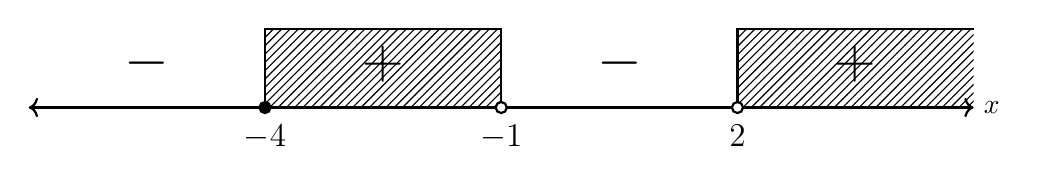
\begin{tikzpicture}
    \draw[thick,<->] (-6,0) -- (6,0) node[right] {$x$};
    \fill[pattern=north east lines] (-3,0) rectangle (0,1);
    \fill[pattern=north east lines] (3,0) rectangle (6,1);
    \draw[thick] (-3,0) -- (-3,1) -- (0,1) -- (0,0);
    \draw[thick] (3,0) -- (3,1) -- (6,1);
    \draw (-3,-0.1) node[below] {\large{$-4$}};
    \draw (0,-0.1) node[below] {\large{$-1$}};
    \draw (3,-0.1) node[below] {\large{$2$}};
    \draw (-4.5,0.2) node[above] {\huge{$-$}};
    \draw (-1.5,0.2) node[above] {\huge{$+$}};
    \draw (1.5,0.2) node[above] {\huge{$-$}};
    \draw (4.5,0.2) node[above] {\huge{$+$}};
    \draw[fill=black, thick] (-3,0) circle (2pt);
    \draw[fill=white, thick] (0,0) circle (2pt);
    \draw[fill=white, thick] (3,0) circle (2pt);
\end{tikzpicture}
        \end{center}
        Karena yang diminta adalah nilai \(x\) yang membuat pertidaksamaan \eqref{ineq:m2} lebih dari atau sama dengan nol, diambil interval yang bertanda positif beserta pembuat nol pembilang ($x=-4$). Pembuat nol penyebut ($x=-1$ dan $x=2$) tidak diikutkan karena membuat ekspresi tidak terdefinisi. Jadi himpunan penyelesaiannya adalah
        \[
        \colorlet{oldcolor}{.}
        \color{red}
        \setlength{\fboxrule}{1pt} \boxed{\color{oldcolor}\{x\in\mathbb{R} : -4\leq x<-1 \;\vee\; x>2\} = [-4,-1)\cup(2,\infty)}\color{oldcolor}.
        \]
    }
    \end{jawab}

    \item Diketahui garis $l_1$ melalui titik $(-1,2)$ dan $(3,4)$.
    \begin{enumerate}
        \item Dapatkan persamaan garis $l_2$ yang melalui titik $(2,1)$ dan tegak lurus dengan garis $l_1$.
        \item Tentukan titik potong garis $l_1$ dan $l_2$.
    \end{enumerate}
    \begin{jawab}[gradien garis, garis tegak lurus, persamaan garis, titik potong garis]{
        \begin{enumerate}
            \item Kemiringan garis yang melalui dua titik $(x_1,y_1)$ dan $(x_2,y_2)$ adalah $m = \frac{y_2 - y_1}{x_2 - x_1}$. Dengan substitusi $(-1,2)$ dan $(3,4)$, diperoleh
            \begin{align*}
                m_1 = \frac{4-2}{3-(-1)} = \frac{2}{4} = \colorlet{oldcolor}{.}
        \color{blue}
        \setlength{\fboxrule}{1pt} \boxed{\color{oldcolor}\frac{1}{2}}\color{oldcolor}.
            \end{align*}
            Dua garis saling tegak lurus jika $\colorlet{oldcolor}{.}
        \color{blue}
        \setlength{\fboxrule}{1pt} \boxed{\color{oldcolor}m_1\cdot m_2=-1}\color{oldcolor}$, sehingga $\frac{1}{2}\cdot m_2=-1$ dan diperoleh $m_2=-2$. Garis $l_2$ melalui titik $(2,1)$, sehingga dengan rumus $y - y_1 = m(x - x_1)$ diperoleh
            \begin{align*}
                y - 1 &= -2(x - 2)\\
                y &= -2x + 5.
            \end{align*}
            Jadi persamaan garis $l_2$ adalah $\colorlet{oldcolor}{.}
        \color{red}
        \setlength{\fboxrule}{1pt} \boxed{\color{oldcolor}y = -2x + 5}\color{oldcolor}$ atau $2x+y=5$.
            \item Terlebih dahulu ditentukan persamaan garis $l_1$, yaitu garis dengan gradien $\frac{1}{2}$ yang melalui titik $(-1,2)$:
            \begin{align*}
                y - 2 = \frac{1}{2}(x + 1) \implies \colorlet{oldcolor}{.}
        \color{blue}
        \setlength{\fboxrule}{1pt} \boxed{\color{oldcolor}y = \frac{1}{2}x + \frac{5}{2}}\color{oldcolor}.
            \end{align*}
            Untuk menentukan titik potong kedua garis, kita samakan persamaan kedua garis, yaitu
            \begin{align*}
                \frac{1}{2}x + \frac{5}{2} &= -2x + 5\\
                x + 5 &= -4x + 10\\
                5x &= 5 \implies x = 1.
            \end{align*}
            Substitusi $x=1$ ke persamaan $l_2$, diperoleh $y=-2(1)+5=3$ (dapat dicek pula $\frac{1}{2}(1)+\frac{5}{2}=3$). Jadi titik potong garis $l_1$ dan $l_2$ adalah $\colorlet{oldcolor}{.}
        \color{red}
        \setlength{\fboxrule}{1pt} \boxed{\color{oldcolor}(1,3)}\color{oldcolor}$.
        \end{enumerate}
    }
    \end{jawab}

    \item Diberikan SPL
    \begin{align*}
        x+2y-z &= 3\\
        2x-y+3z &= 6\\
        -x+y+2z &= 5
    \end{align*}
    \begin{enumerate}
        \item Nyatakan SPL tersebut dalam bentuk persamaan matriks $A\mathbf{x}=b$.
        \item Menggunakan eliminasi Gauss-Jordan, carilah solusi (jika ada) dari SPL tersebut.
    \end{enumerate}
    \begin{jawab}[sistem persamaan linear, matriks, eliminasi Gauss-Jordan]{
        \begin{enumerate}
            \item Koefisien dari variabel $x,y,z$ pada setiap persamaan disusun menjadi matriks $A$, variabelnya menjadi vektor $\mathbf{x}$, dan ruas kanan menjadi vektor $b$. Diperoleh
            \begin{align*}
                \colorlet{oldcolor}{.}
        \color{red}
        \setlength{\fboxrule}{1pt} \boxed{\color{oldcolor}\underbrace{\begin{bmatrix}
                    1 & 2 & -1\\
                    2 & -1 & 3\\
                    -1 & 1 & 2
                \end{bmatrix}}_{A}
                \underbrace{\begin{bmatrix}
                    x\\ y\\ z
                \end{bmatrix}}_{\mathbf{x}}
                =
                \underbrace{\begin{bmatrix}
                    3\\ 6\\ 5
                \end{bmatrix}}_{b}}\color{oldcolor}.
            \end{align*}
            \item Dibentuk matriks lengkap (\textit{augmented matrix}) $[A\,|\,b]$, kemudian dilakukan operasi baris elementer (OBE) sampai terbentuk matriks eselon baris tereduksi.
            \begin{align*}
                &\left[\begin{array}{ccc|c}
                    1 & 2 & -1 & 3\\
                    2 & -1 & 3 & 6\\
                    -1 & 1 & 2 & 5
                \end{array}\right]
                \xrightarrow[R_3 + R_1]{R_2 - 2R_1}
                \left[\begin{array}{ccc|c}
                    1 & 2 & -1 & 3\\
                    0 & -5 & 5 & 0\\
                    0 & 3 & 1 & 8
                \end{array}\right]
                \xrightarrow{-\frac{1}{5}R_2}
                \left[\begin{array}{ccc|c}
                    1 & 2 & -1 & 3\\
                    0 & 1 & -1 & 0\\
                    0 & 3 & 1 & 8
                \end{array}\right]\\
                &\xrightarrow[R_3 - 3R_2]{R_1 - 2R_2}
                \left[\begin{array}{ccc|c}
                    1 & 0 & 1 & 3\\
                    0 & 1 & -1 & 0\\
                    0 & 0 & 4 & 8
                \end{array}\right]
                \xrightarrow{\frac{1}{4}R_3}
                \left[\begin{array}{ccc|c}
                    1 & 0 & 1 & 3\\
                    0 & 1 & -1 & 0\\
                    0 & 0 & 1 & 2
                \end{array}\right]
                \xrightarrow[R_2 + R_3]{R_1 - R_3}
                \left[\begin{array}{ccc|c}
                    1 & 0 & 0 & 1\\
                    0 & 1 & 0 & 2\\
                    0 & 0 & 1 & 2
                \end{array}\right]
            \end{align*}
            Matriks terakhir sudah berbentuk eselon baris tereduksi dan setiap kolom variabel memiliki pivot, sehingga SPL memiliki solusi tunggal, yaitu $\colorlet{oldcolor}{.}
        \color{blue}
        \setlength{\fboxrule}{1pt} \boxed{\color{oldcolor}x=1}\color{oldcolor}$, $\colorlet{oldcolor}{.}
        \color{blue}
        \setlength{\fboxrule}{1pt} \boxed{\color{oldcolor}y=2}\color{oldcolor}$, dan $\colorlet{oldcolor}{.}
        \color{blue}
        \setlength{\fboxrule}{1pt} \boxed{\color{oldcolor}z=2}\color{oldcolor}$.\\
            Sebagai pengecekan, $1+2(2)-2=3$, $2(1)-2+3(2)=6$, dan $-1+2+2(2)=5$, sesuai dengan SPL. Jadi solusi dari SPL tersebut adalah $\colorlet{oldcolor}{.}
        \color{red}
        \setlength{\fboxrule}{1pt} \boxed{\color{oldcolor}(x,y,z)=(1,2,2)}\color{oldcolor}$.
        \end{enumerate}
    }
    \end{jawab}

    \item Diketahui fungsi $f(x)=x^2-4x-5$.
    \begin{enumerate}
        \item Dapatkan domain dan range dari $f(x)$.
        \item Sketsa grafik $f(x)$ beserta titik puncak dan titik potongnya dengan sumbu koordinat.
    \end{enumerate}
    \begin{jawab}[fungsi kuadrat, melengkapkan kuadrat, domain dan range, sketsa grafik]{
        \begin{enumerate}
            \item Karena $f$ adalah fungsi polinomial (fungsi kuadrat), maka $f$ terdefinisi untuk setiap bilangan real, sehingga $\colorlet{oldcolor}{.}
        \color{red}
        \setlength{\fboxrule}{1pt} \boxed{\color{oldcolor}D(f)=\mathbb{R}}\color{oldcolor}$. Selanjutnya, dengan melengkapkan kuadrat, diperoleh
            \begin{align*}
                f(x) = x^2-4x-5 = (x^2-4x+4)-4-5 = \colorlet{oldcolor}{.}
        \color{blue}
        \setlength{\fboxrule}{1pt} \boxed{\color{oldcolor}(x-2)^2-9}\color{oldcolor}.
            \end{align*}
            Karena $(x-2)^2\geq 0$ untuk setiap $x$, maka $f(x)\geq -9$, dengan nilai minimum $-9$ dicapai saat $x=2$. Grafiknya terbuka ke atas sehingga nilainya membesar tanpa batas. Jadi
            \begin{align*}
                \colorlet{oldcolor}{.}
        \color{red}
        \setlength{\fboxrule}{1pt} \boxed{\color{oldcolor}R(f)=\{y\in\mathbb{R} : y\geq -9\}=[-9,\infty)}\color{oldcolor}.
            \end{align*}
            \item Dari (a), titik puncak parabola adalah $\colorlet{oldcolor}{.}
        \color{blue}
        \setlength{\fboxrule}{1pt} \boxed{\color{oldcolor}(2,-9)}\color{oldcolor}$, dan karena koefisien $x^2$ positif, parabola terbuka ke atas.
            \begin{itemize}
                \item Titik potong dengan sumbu-$x$ ($y=0$): $x^2-4x-5=(x-5)(x+1)=0$, sehingga $x=5$ atau $x=-1$, yaitu titik $\colorlet{oldcolor}{.}
        \color{blue}
        \setlength{\fboxrule}{1pt} \boxed{\color{oldcolor}(-1,0)}\color{oldcolor}$ dan $\colorlet{oldcolor}{.}
        \color{blue}
        \setlength{\fboxrule}{1pt} \boxed{\color{oldcolor}(5,0)}\color{oldcolor}$.
                \item Titik potong dengan sumbu-$y$ ($x=0$): $f(0)=-5$, yaitu titik $\colorlet{oldcolor}{.}
        \color{blue}
        \setlength{\fboxrule}{1pt} \boxed{\color{oldcolor}(0,-5)}\color{oldcolor}$.
            \end{itemize}
            Sketsa grafiknya adalah sebagai berikut:
            \begin{center}
                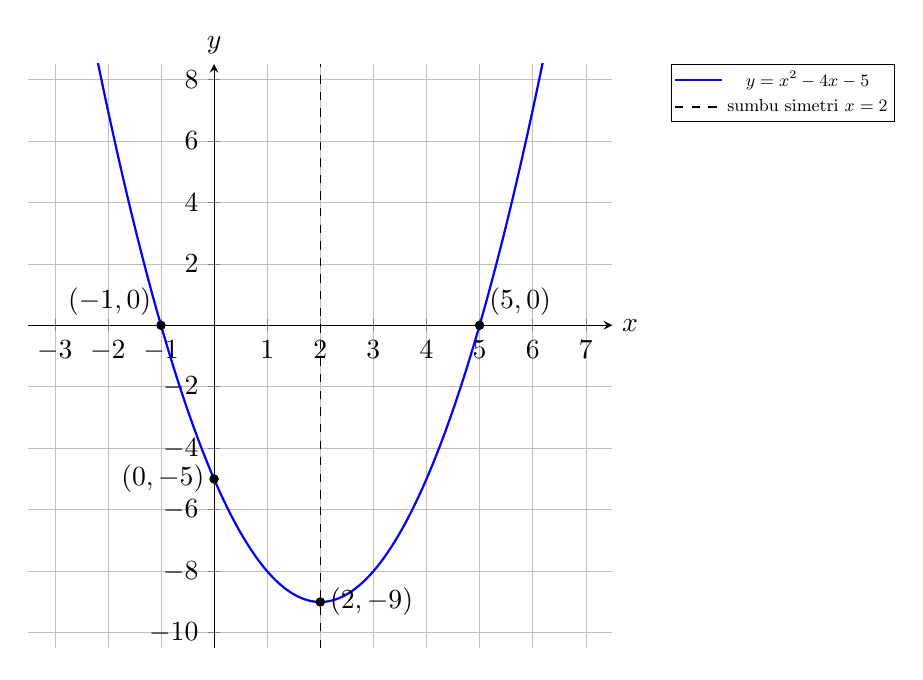
\begin{tikzpicture}
                    \begin{axis}[
        axis lines = middle,
        xlabel = $x$,
        ylabel = {$y$},
        grid=both,
        grid style={line width=.1pt, draw=gray!10},
        major grid style={line width=.2pt,draw=gray!50},
        x label style={anchor=west}, % label x ke kanan
        y label style={anchor=south}, % label y ke atas
        samples=200,
        legend style={
                at={(1.1,1)},
                anchor=north west,
                font=\small,         % mengecilkan ukuran font
                row sep=1pt,         % jarak antar baris legend
                inner sep=1pt,       % margin dalam kotak legend
                nodes={scale=0.7}    % skalakan isi legend
            },
        xtick={-3,-2,...,7},
        ytick={-10,-8,...,8},
        xmin=-3.5, xmax=7.5,
        ymin=-10.5, ymax=8.5,
        width=9cm,
        height=9cm
    ]
\addplot[domain=-2.4:6.4, color=blue, thick] {x^2-4*x-5};
\addlegendentry{$y=x^2-4x-5$}
\addplot[color=black, dashed] coordinates {(2,-10.5) (2,8.5)};
\addlegendentry{sumbu simetri $x=2$}
\draw[fill=black] (2,-9) circle (1.5pt) node[right] {$(2,-9)$};
\draw[fill=black] (-1,0) circle (1.5pt) node[above left] {$(-1,0)$};
\draw[fill=black] (5,0) circle (1.5pt) node[above right] {$(5,0)$};
\draw[fill=black] (0,-5) circle (1.5pt) node[left] {$(0,-5)$};
\end{axis}
                \end{tikzpicture}
            \end{center}
        \end{enumerate}
    }
    \end{jawab}

    \item Diberikan sistem persamaan fungsi permintaan dan penawaran (\textit{supply and demand})
    \begin{align*}
        3P &= -Q_d+150\\
        2P &= Q_s+25
    \end{align*}
    dengan $P,Q_d,Q_s$ masing-masing adalah harga, jumlah permintaan (\textit{demand}), dan jumlah penawaran (\textit{supply}).
    \begin{enumerate}
        \item Tentukan harga dan jumlah barang di titik equilibrium.
        \item Misalkan pemerintah memberikan pajak sebesar 5 untuk masing-masing barang. Tentukan persamaan fungsi penawaran setelah dikenakan pajak, titik equilibrium yang baru, dan pembagian pembayaran pajaknya.
        \item Gambarkan/sket kurva permintaan dan penawaran (sebelum dan sesudah pajak) beserta titik keseimbangannya.
    \end{enumerate}
    \begin{jawab}[fungsi permintaan, fungsi penawaran, titik keseimbangan pasar, pajak per unit]{~\\
        Dari sistem persamaan yang diberikan, fungsi permintaan dan penawaran dapat ditulis sebagai
        \begin{align*}
            \colorlet{oldcolor}{.}
        \color{blue}
        \setlength{\fboxrule}{1pt} \boxed{\color{oldcolor}Q_d = 150 - 3P}\color{oldcolor} \quad\text{dan}\quad \colorlet{oldcolor}{.}
        \color{blue}
        \setlength{\fboxrule}{1pt} \boxed{\color{oldcolor}Q_s = 2P - 25}\color{oldcolor}.
        \end{align*}
        \begin{enumerate}
            \item Titik keseimbangan (\textit{equilibrium}) terjadi saat jumlah permintaan sama dengan jumlah penawaran, yaitu $\colorlet{oldcolor}{.}
        \color{blue}
        \setlength{\fboxrule}{1pt} \boxed{\color{oldcolor}Q_d=Q_s}\color{oldcolor}$. Diperoleh
            \begin{align*}
                150 - 3P &= 2P - 25\\
                175 &= 5P\\
                P &= 35.
            \end{align*}
            Substitusi $P=35$ ke fungsi permintaan, diperoleh $Q = 150 - 3(35) = 150 - 105 = 45$ (dapat dicek pula $Q_s=2(35)-25=45$). Jadi titik keseimbangannya adalah $\colorlet{oldcolor}{.}
        \color{red}
        \setlength{\fboxrule}{1pt} \boxed{\color{oldcolor}E(Q,P)=(45,35)}\color{oldcolor}$, yaitu harga keseimbangan $35$ dengan jumlah barang $45$ unit.
            \item Pajak per unit $t=5$ dibebankan kepada produsen, sehingga untuk menawarkan jumlah barang yang sama, produsen menaikkan harga sebesar $5$. Dari fungsi penawaran semula $P=\frac{Q+25}{2}$, fungsi penawaran setelah pajak adalah
            \begin{align*}
                P = \frac{Q+25}{2} + 5 \iff 2P = Q + 35 \iff \colorlet{oldcolor}{.}
        \color{red}
        \setlength{\fboxrule}{1pt} \boxed{\color{oldcolor}Q_s' = 2P - 35}\color{oldcolor}.
            \end{align*}
            Titik keseimbangan baru diperoleh dari $Q_d=Q_s'$, yaitu
            \begin{align*}
                150 - 3P &= 2P - 35\\
                185 &= 5P\\
                P &= 37,
            \end{align*}
            dan $Q = 150 - 3(37) = 150 - 111 = 39$. Jadi titik keseimbangan setelah pajak adalah
            \begin{align*}
                \colorlet{oldcolor}{.}
        \color{red}
        \setlength{\fboxrule}{1pt} \boxed{\color{oldcolor}E'(Q,P)=(39,37)}\color{oldcolor}.
            \end{align*}
            Selanjutnya, pembagian pembayaran pajak per unit adalah sebagai berikut.
            \begin{itemize}
                \item Pajak yang ditanggung konsumen per unit adalah kenaikan harga yang dibayar konsumen, yaitu $37-35=2$.
                \item Pajak yang ditanggung produsen per unit adalah sisanya, yaitu $5-2=3$.
            \end{itemize}
            Dengan jumlah barang setelah pajak sebanyak $39$ unit, total pajak yang diterima pemerintah adalah $5\times 39=195$, dengan pembagian
            \[
            \colorlet{oldcolor}{.}
        \color{red}
        \setlength{\fboxrule}{1pt} \boxed{\color{oldcolor}\text{konsumen: } 2\times 39 = 78, \quad \text{produsen: } 3\times 39 = 117}\color{oldcolor}.
            \]
            \item Dalam ekonomi, sumbu mendatar menyatakan jumlah barang $Q$ dan sumbu tegak menyatakan harga $P$. Sebagai bantuan menggambar:
            \begin{itemize}
                \item Kurva permintaan $P=\frac{150-Q}{3}$ melalui titik $(0,50)$ dan $(150,0)$, dan turun dari kiri ke kanan.
                \item Kurva penawaran sebelum pajak $P=\frac{Q+25}{2}$ melalui titik $(0;12{,}5)$ dan $(45,35)$, dan naik dari kiri ke kanan.
                \item Kurva penawaran setelah pajak $P=\frac{Q+35}{2}$ melalui titik $(0;17{,}5)$ dan $(39,37)$, yaitu kurva penawaran semula yang bergeser $5$ satuan ke atas.
            \end{itemize}
            Sketsa kurva permintaan, penawaran, dan titik keseimbangannya adalah sebagai berikut
            \begin{center}
                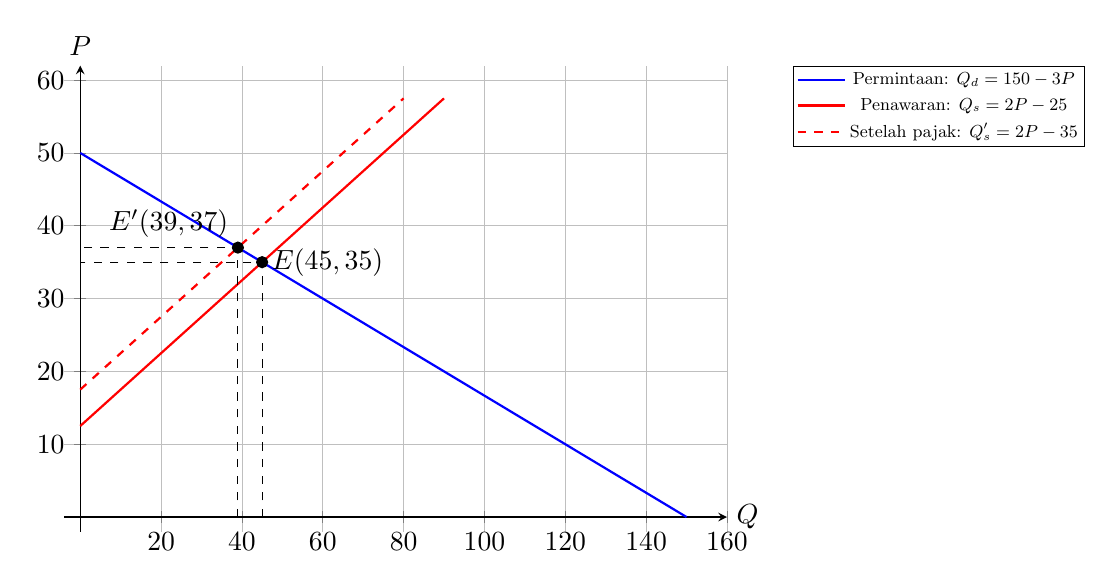
\begin{tikzpicture}
                    \begin{axis}[
        axis lines = middle,
        xlabel = $x$,
        ylabel = {$y$},
        grid=both,
        grid style={line width=.1pt, draw=gray!10},
        major grid style={line width=.2pt,draw=gray!50},
        x label style={anchor=west}, % label x ke kanan
        y label style={anchor=south}, % label y ke atas
        samples=200,
        legend style={
                at={(1.1,1)},
                anchor=north west,
                font=\small,         % mengecilkan ukuran font
                row sep=1pt,         % jarak antar baris legend
                inner sep=1pt,       % margin dalam kotak legend
                nodes={scale=0.7}    % skalakan isi legend
            },
        xlabel = $Q$,
        ylabel = {$P$},
        xtick={0,20,...,160},
        ytick={0,10,...,60},
        xmin=-4, xmax=160,
        ymin=-2, ymax=62,
        width=10cm,
        height=7.5cm
    ]
\addplot[domain=0:150, color=blue, thick, samples=2] {(150-x)/3};
\addlegendentry{Permintaan: $Q_d=150-3P$}
\addplot[domain=0:90, color=red, thick, samples=2] {(x+25)/2};
\addlegendentry{Penawaran: $Q_s=2P-25$}
\addplot[domain=0:80, color=red, thick, dashed, samples=2] {(x+35)/2};
\addlegendentry{Setelah pajak: $Q_s'=2P-35$}
\draw[fill=black] (45,35) circle (2pt) node[right] {$E(45,35)$};
\draw[fill=black] (39,37) circle (2pt) node[above left] {$E'(39,37)$};
\draw[dashed] (45,0) -- (45,35) -- (0,35);
\draw[dashed] (39,0) -- (39,37) -- (0,37);
\end{axis}
                \end{tikzpicture}
            \end{center}
        \end{enumerate}
    }
    \end{jawab}
\end{enumerate}

\newpage

%%%%%%%%%%%%%%%%%%%%%%%%%%%%%%%%%%%%%%%%%%%%%%%%%%%%%%%%%%%%%%%%%%%%%%%%%%%%%%
% M2-iup
\kopsoalmatiup{M2-iup}{8, 9}{Information Systems, Business Management}{Friday, 07.00-09.30}{11}
\begin{enumerate}
    \item Find the solution set of $\dfrac{3}{x+2}\leq\dfrac{1}{x-2}$.
    \begin{jawab}[pertidaksamaan rasional, pecahan, garis bilangan, notasi interval]{~\\
        Untuk menyelesaikan pertidaksamaan rasional, pastikan ruas kanan sudah bernilai nol (jangan dikali silang, karena tanda penyebutnya belum diketahui). Dengan mengurangkan \(\frac{1}{x-2}\) dari kedua ruas, didapatkan
        \[
        \frac{3}{x+2} - \frac{1}{x-2} \leq 0
        \]
        Selanjutnya, dengan menyamakan penyebut dan menyederhanakan bentuknya, diperoleh
        \begin{align}
            \frac{3(x-2)-(x+2)}{(x+2)(x-2)} &\leq 0\nonumber\\
            \frac{3x-6-x-2}{(x+2)(x-2)} &\leq 0\nonumber \\
            \frac{2(x-4)}{(x+2)(x-2)} &\leq 0 \label{ineq:m2iup}
        \end{align}
        Didapatkan pembuat nol dari faktor-faktornya adalah
        \begin{align*}
            x-4 = 0 \quad &\vee\quad  x+2 = 0 \quad\vee\quad x-2=0\\
            \colorlet{oldcolor}{.}
        \color{blue}
        \setlength{\fboxrule}{1pt} \boxed{\color{oldcolor}x=4}\color{oldcolor} \quad &\vee\quad \colorlet{oldcolor}{.}
        \color{blue}
        \setlength{\fboxrule}{1pt} \boxed{\color{oldcolor}x=-2}\color{oldcolor} \quad\vee\quad \colorlet{oldcolor}{.}
        \color{blue}
        \setlength{\fboxrule}{1pt} \boxed{\color{oldcolor}x=2}\color{oldcolor}
        \end{align*}
        Selanjutnya, dibuat garis bilangan dan dilakukan uji titik pada ekspresi \eqref{ineq:m2iup} sebagai berikut
        \begin{itemize}
            \item Untuk \(x < -2\), misalkan \(x = -3\):
            \[
            \frac{2(-3-4)}{(-3+2)(-3-2)} = \frac{-14}{(-1)(-5)} = \frac{-14}{5} < 0
            \]
            \item Untuk \(-2 < x < 2\), misalkan \(x = 0\):
            \[
            \frac{2(0-4)}{(0+2)(0-2)} = \frac{-8}{-4} > 0
            \]
            \item Untuk \(2 < x < 4\), misalkan \(x = 3\):
            \[
            \frac{2(3-4)}{(3+2)(3-2)} = \frac{-2}{5} < 0
            \]
            \item Untuk \(x > 4\), misalkan \(x = 5\):
            \[
            \frac{2(5-4)}{(5+2)(5-2)} = \frac{2}{21} > 0
            \]
        \end{itemize}
        \begin{center}
           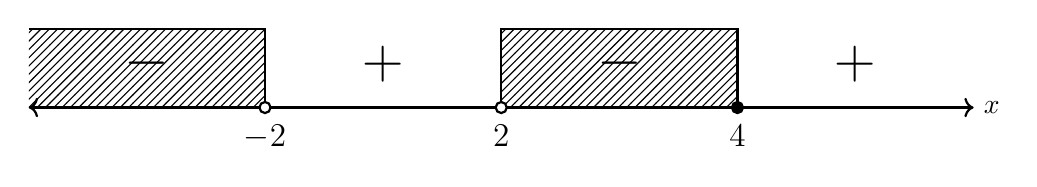
\begin{tikzpicture}
    \draw[thick,<->] (-6,0) -- (6,0) node[right] {$x$};
    \fill[pattern=north east lines] (-6,0) rectangle (-3,1);
    \fill[pattern=north east lines] (0,0) rectangle (3,1);
    \draw[thick] (-6,1) -- (-3,1) -- (-3,0);
    \draw[thick] (0,0) -- (0,1) -- (3,1) -- (3,0);
    \draw (-3,-0.1) node[below] {\large{$-2$}};
    \draw (0,-0.1) node[below] {\large{$2$}};
    \draw (3,-0.1) node[below] {\large{$4$}};
    \draw (-4.5,0.2) node[above] {\huge{$-$}};
    \draw (-1.5,0.2) node[above] {\huge{$+$}};
    \draw (1.5,0.2) node[above] {\huge{$-$}};
    \draw (4.5,0.2) node[above] {\huge{$+$}};
    \draw[fill=white, thick] (-3,0) circle (2pt);
    \draw[fill=white, thick] (0,0) circle (2pt);
    \draw[fill=black, thick] (3,0) circle (2pt);
\end{tikzpicture}
        \end{center}
        Karena yang diminta adalah nilai \(x\) yang membuat pertidaksamaan \eqref{ineq:m2iup} kurang dari atau sama dengan nol, diambil interval yang bertanda negatif beserta pembuat nol pembilang ($x=4$). Pembuat nol penyebut ($x=-2$ dan $x=2$) tidak diikutkan karena membuat ekspresi tidak terdefinisi. Jadi himpunan penyelesaiannya adalah
        \[
        \colorlet{oldcolor}{.}
        \color{red}
        \setlength{\fboxrule}{1pt} \boxed{\color{oldcolor}\{x\in\mathbb{R} : x<-2 \;\vee\; 2<x\leq 4\} = (-\infty,-2)\cup(2,4]}\color{oldcolor}.
        \]
    }
    \end{jawab}

    \item \begin{enumerate}
        \item Determine the value of $k$ such that the line $\ell_1: kx+2y=7$ is perpendicular to the line $\ell_2: 4x-6y=1$.
        \item Using the value of $k$ in (a), find the equation of the line passing through $(1,2)$ that is parallel to $\ell_1$.
    \end{enumerate}
    \begin{jawab}[gradien garis, garis tegak lurus, garis sejajar, persamaan garis]{
        \begin{enumerate}
            \item Ingat kembali bahwa garis $ax+by=c$ dapat ditulis menjadi $y=-\frac{a}{b}x+\frac{c}{b}$, sehingga gradiennya adalah $m=-\frac{a}{b}$. Diperoleh
            \begin{align*}
                \ell_1: kx+2y=7 \implies y = -\frac{k}{2}x + \frac{7}{2} \implies \colorlet{oldcolor}{.}
        \color{blue}
        \setlength{\fboxrule}{1pt} \boxed{\color{oldcolor}m_1 = -\frac{k}{2}}\color{oldcolor},\\
                \ell_2: 4x-6y=1 \implies y = \frac{2}{3}x - \frac{1}{6} \implies \colorlet{oldcolor}{.}
        \color{blue}
        \setlength{\fboxrule}{1pt} \boxed{\color{oldcolor}m_2 = \frac{2}{3}}\color{oldcolor}.
            \end{align*}
            Dua garis saling tegak lurus jika $m_1\cdot m_2=-1$, sehingga
            \begin{align*}
                -\frac{k}{2}\cdot\frac{2}{3} = -1 \implies -\frac{k}{3} = -1 \implies k=\colorlet{oldcolor}{.}
        \color{red}
        \setlength{\fboxrule}{1pt} \boxed{\color{oldcolor}3}\color{oldcolor}.
            \end{align*}
            \item Untuk $k=3$, garis $\ell_1$ adalah $3x+2y=7$ dengan gradien $m_1=-\frac{3}{2}$. Dua garis sejajar memiliki gradien yang sama, sehingga garis yang dicari memiliki gradien $-\frac{3}{2}$ dan melalui titik $(1,2)$. Dengan rumus $y - y_1 = m(x - x_1)$ diperoleh
            \begin{align*}
                y - 2 &= -\frac{3}{2}(x - 1)\\
                y &= -\frac{3}{2}x + \frac{3}{2} + 2\\
                y &= -\frac{3}{2}x + \frac{7}{2}.
            \end{align*}
            Jadi persamaan garisnya adalah $\colorlet{oldcolor}{.}
        \color{red}
        \setlength{\fboxrule}{1pt} \boxed{\color{oldcolor}y = -\frac{3}{2}x + \frac{7}{2}}\color{oldcolor}$ atau $3x+2y=7$.\\
            \textit{Catatan:} garis yang diperoleh ternyata sama dengan $\ell_1$ itu sendiri, karena titik $(1,2)$ terletak pada $\ell_1$, yaitu $3(1)+2(2)=7$. Satu-satunya garis yang sejajar $\ell_1$ dan melalui titik pada $\ell_1$ adalah $\ell_1$ sendiri (garis yang berimpit).
        \end{enumerate}
    }
    \end{jawab}

    \item Given the system of linear equations
    \begin{align*}
        2x+y-z &= 3\\
        x-y+2z &= 1\\
        3x+2y+z &= 8
    \end{align*}
    \begin{enumerate}
        \item Write the system in the matrix equation form $A\mathbf{x}=b$.
        \item Using Gauss-Jordan elimination, find the solution (if any) of the system.
    \end{enumerate}
    \begin{jawab}[sistem persamaan linear, matriks, eliminasi Gauss-Jordan]{
        \begin{enumerate}
            \item Koefisien dari variabel $x,y,z$ pada setiap persamaan disusun menjadi matriks $A$, variabelnya menjadi vektor $\mathbf{x}$, dan ruas kanan menjadi vektor $b$. Diperoleh
            \begin{align*}
                \colorlet{oldcolor}{.}
        \color{red}
        \setlength{\fboxrule}{1pt} \boxed{\color{oldcolor}\underbrace{\begin{bmatrix}
                    2 & 1 & -1\\
                    1 & -1 & 2\\
                    3 & 2 & 1
                \end{bmatrix}}_{A}
                \underbrace{\begin{bmatrix}
                    x\\ y\\ z
                \end{bmatrix}}_{\mathbf{x}}
                =
                \underbrace{\begin{bmatrix}
                    3\\ 1\\ 8
                \end{bmatrix}}_{b}}\color{oldcolor}.
            \end{align*}
            \item Dibentuk matriks lengkap (\textit{augmented matrix}) $[A\,|\,b]$, kemudian dilakukan operasi baris elementer (OBE) sampai terbentuk matriks eselon baris tereduksi. Agar pivot pertama bernilai $1$, baris pertama dan kedua ditukar terlebih dahulu.
            \begin{align*}
                &\left[\begin{array}{ccc|c}
                    2 & 1 & -1 & 3\\
                    1 & -1 & 2 & 1\\
                    3 & 2 & 1 & 8
                \end{array}\right]
                \xrightarrow{R_1 \leftrightarrow R_2}
                \left[\begin{array}{ccc|c}
                    1 & -1 & 2 & 1\\
                    2 & 1 & -1 & 3\\
                    3 & 2 & 1 & 8
                \end{array}\right]
                \xrightarrow[R_3 - 3R_1]{R_2 - 2R_1}
                \left[\begin{array}{ccc|c}
                    1 & -1 & 2 & 1\\
                    0 & 3 & -5 & 1\\
                    0 & 5 & -5 & 5
                \end{array}\right]\\
                &\xrightarrow[R_2 \leftrightarrow R_3]{\frac{1}{5}R_3}
                \left[\begin{array}{ccc|c}
                    1 & -1 & 2 & 1\\
                    0 & 1 & -1 & 1\\
                    0 & 3 & -5 & 1
                \end{array}\right]
                \xrightarrow[R_3 - 3R_2]{R_1 + R_2}
                \left[\begin{array}{ccc|c}
                    1 & 0 & 1 & 2\\
                    0 & 1 & -1 & 1\\
                    0 & 0 & -2 & -2
                \end{array}\right]
                \xrightarrow{-\frac{1}{2}R_3}
                \left[\begin{array}{ccc|c}
                    1 & 0 & 1 & 2\\
                    0 & 1 & -1 & 1\\
                    0 & 0 & 1 & 1
                \end{array}\right]\\
                &\xrightarrow[R_2 + R_3]{R_1 - R_3}
                \left[\begin{array}{ccc|c}
                    1 & 0 & 0 & 1\\
                    0 & 1 & 0 & 2\\
                    0 & 0 & 1 & 1
                \end{array}\right]
            \end{align*}
            Matriks terakhir sudah berbentuk eselon baris tereduksi dan setiap kolom variabel memiliki pivot, sehingga SPL memiliki solusi tunggal, yaitu $\colorlet{oldcolor}{.}
        \color{blue}
        \setlength{\fboxrule}{1pt} \boxed{\color{oldcolor}x=1}\color{oldcolor}$, $\colorlet{oldcolor}{.}
        \color{blue}
        \setlength{\fboxrule}{1pt} \boxed{\color{oldcolor}y=2}\color{oldcolor}$, dan $\colorlet{oldcolor}{.}
        \color{blue}
        \setlength{\fboxrule}{1pt} \boxed{\color{oldcolor}z=1}\color{oldcolor}$.\\
            Sebagai pengecekan, $2(1)+2-1=3$, $1-2+2(1)=1$, dan $3(1)+2(2)+1=8$, sesuai dengan SPL. Jadi solusi dari SPL tersebut adalah $\colorlet{oldcolor}{.}
        \color{red}
        \setlength{\fboxrule}{1pt} \boxed{\color{oldcolor}(x,y,z)=(1,2,1)}\color{oldcolor}$.
        \end{enumerate}
    }
    \end{jawab}

    \item Given the function $f(x)=-x^2+4x+5$.
    \begin{enumerate}
        \item Find the domain and range of $f(x)$.
        \item Sketch the graph of $f(x)$ including its vertex and its intersection points with the coordinate axes.
    \end{enumerate}
    \begin{jawab}[fungsi kuadrat, melengkapkan kuadrat, domain dan range, sketsa grafik]{
        \begin{enumerate}
            \item Karena $f$ adalah fungsi polinomial (fungsi kuadrat), maka $f$ terdefinisi untuk setiap bilangan real, sehingga $\colorlet{oldcolor}{.}
        \color{red}
        \setlength{\fboxrule}{1pt} \boxed{\color{oldcolor}D(f)=\mathbb{R}}\color{oldcolor}$. Selanjutnya, dengan melengkapkan kuadrat, diperoleh
            \begin{align*}
                f(x) = -x^2+4x+5 = -(x^2-4x+4)+4+5 = \colorlet{oldcolor}{.}
        \color{blue}
        \setlength{\fboxrule}{1pt} \boxed{\color{oldcolor}-(x-2)^2+9}\color{oldcolor}.
            \end{align*}
            Karena $-(x-2)^2\leq 0$ untuk setiap $x$, maka $f(x)\leq 9$, dengan nilai maksimum $9$ dicapai saat $x=2$. Grafiknya terbuka ke bawah sehingga nilainya mengecil tanpa batas. Jadi
            \begin{align*}
                \colorlet{oldcolor}{.}
        \color{red}
        \setlength{\fboxrule}{1pt} \boxed{\color{oldcolor}R(f)=\{y\in\mathbb{R} : y\leq 9\}=(-\infty,9]}\color{oldcolor}.
            \end{align*}
            \item Dari (a), titik puncak parabola adalah $\colorlet{oldcolor}{.}
        \color{blue}
        \setlength{\fboxrule}{1pt} \boxed{\color{oldcolor}(2,9)}\color{oldcolor}$, dan karena koefisien $x^2$ negatif, parabola terbuka ke bawah.
            \begin{itemize}
                \item Titik potong dengan sumbu-$x$ ($y=0$): $-x^2+4x+5=-(x-5)(x+1)=0$, sehingga $x=5$ atau $x=-1$, yaitu titik $\colorlet{oldcolor}{.}
        \color{blue}
        \setlength{\fboxrule}{1pt} \boxed{\color{oldcolor}(-1,0)}\color{oldcolor}$ dan $\colorlet{oldcolor}{.}
        \color{blue}
        \setlength{\fboxrule}{1pt} \boxed{\color{oldcolor}(5,0)}\color{oldcolor}$.
                \item Titik potong dengan sumbu-$y$ ($x=0$): $f(0)=5$, yaitu titik $\colorlet{oldcolor}{.}
        \color{blue}
        \setlength{\fboxrule}{1pt} \boxed{\color{oldcolor}(0,5)}\color{oldcolor}$.
            \end{itemize}
            Sketsa grafiknya adalah sebagai berikut:
            \begin{center}
                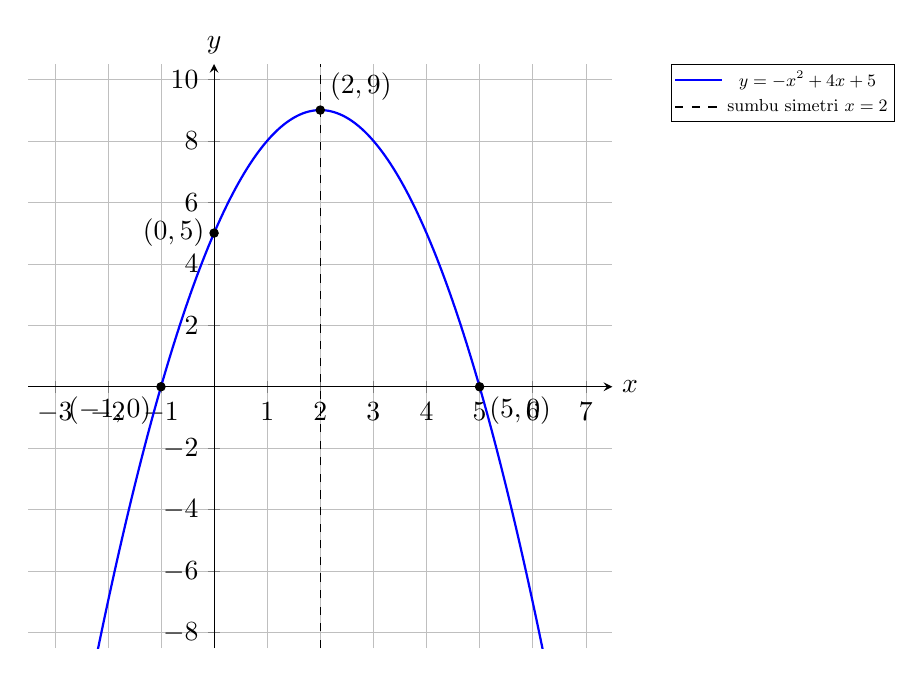
\begin{tikzpicture}
                    \begin{axis}[
        axis lines = middle,
        xlabel = $x$,
        ylabel = {$y$},
        grid=both,
        grid style={line width=.1pt, draw=gray!10},
        major grid style={line width=.2pt,draw=gray!50},
        x label style={anchor=west}, % label x ke kanan
        y label style={anchor=south}, % label y ke atas
        samples=200,
        legend style={
                at={(1.1,1)},
                anchor=north west,
                font=\small,         % mengecilkan ukuran font
                row sep=1pt,         % jarak antar baris legend
                inner sep=1pt,       % margin dalam kotak legend
                nodes={scale=0.7}    % skalakan isi legend
            },
        xtick={-3,-2,...,7},
        ytick={-8,-6,...,10},
        xmin=-3.5, xmax=7.5,
        ymin=-8.5, ymax=10.5,
        width=9cm,
        height=9cm
    ]
\addplot[domain=-2.3:6.3, color=blue, thick] {-x^2+4*x+5};
\addlegendentry{$y=-x^2+4x+5$}
\addplot[color=black, dashed] coordinates {(2,-8.5) (2,10.5)};
\addlegendentry{sumbu simetri $x=2$}
\draw[fill=black] (2,9) circle (1.5pt) node[above right] {$(2,9)$};
\draw[fill=black] (-1,0) circle (1.5pt) node[below left] {$(-1,0)$};
\draw[fill=black] (5,0) circle (1.5pt) node[below right] {$(5,0)$};
\draw[fill=black] (0,5) circle (1.5pt) node[left] {$(0,5)$};
\end{axis}
                \end{tikzpicture}
            \end{center}
        \end{enumerate}
    }
    \end{jawab}

    \item Given the demand and supply functions
    \begin{align*}
        4P &= -Q_d+140\\
        3P &= Q_s+14
    \end{align*}
    where $P,Q_d,Q_s$ are the price, the quantity demanded, and the quantity supplied, respectively.
    \begin{enumerate}
        \item Find the equilibrium price and quantity.
        \item Suppose the government imposes a tax of 7 per unit. Find the supply function after tax, the new equilibrium point, and how the tax burden is shared between consumers and producers.
        \item Sketch the demand and supply curves (before and after tax) and the equilibrium points.
    \end{enumerate}
    \begin{jawab}[fungsi permintaan, fungsi penawaran, titik keseimbangan pasar, pajak per unit]{~\\
        Dari sistem persamaan yang diberikan, fungsi permintaan dan penawaran dapat ditulis sebagai
        \begin{align*}
            \colorlet{oldcolor}{.}
        \color{blue}
        \setlength{\fboxrule}{1pt} \boxed{\color{oldcolor}Q_d = 140 - 4P}\color{oldcolor} \quad\text{dan}\quad \colorlet{oldcolor}{.}
        \color{blue}
        \setlength{\fboxrule}{1pt} \boxed{\color{oldcolor}Q_s = 3P - 14}\color{oldcolor}.
        \end{align*}
        \begin{enumerate}
            \item Titik keseimbangan (\textit{equilibrium}) terjadi saat jumlah permintaan sama dengan jumlah penawaran, yaitu $\colorlet{oldcolor}{.}
        \color{blue}
        \setlength{\fboxrule}{1pt} \boxed{\color{oldcolor}Q_d=Q_s}\color{oldcolor}$. Diperoleh
            \begin{align*}
                140 - 4P &= 3P - 14\\
                154 &= 7P\\
                P &= 22.
            \end{align*}
            Substitusi $P=22$ ke fungsi permintaan, diperoleh $Q = 140 - 4(22) = 140 - 88 = 52$ (dapat dicek pula $Q_s=3(22)-14=52$). Jadi titik keseimbangannya adalah $\colorlet{oldcolor}{.}
        \color{red}
        \setlength{\fboxrule}{1pt} \boxed{\color{oldcolor}E(Q,P)=(52,22)}\color{oldcolor}$, yaitu harga keseimbangan $22$ dengan jumlah barang $52$ unit.
            \item Pajak per unit $t=7$ dibebankan kepada produsen, sehingga untuk menawarkan jumlah barang yang sama, produsen menaikkan harga sebesar $7$. Dari fungsi penawaran semula $P=\frac{Q+14}{3}$, fungsi penawaran setelah pajak adalah
            \begin{align*}
                P = \frac{Q+14}{3} + 7 \iff 3P = Q + 35 \iff \colorlet{oldcolor}{.}
        \color{red}
        \setlength{\fboxrule}{1pt} \boxed{\color{oldcolor}Q_s' = 3P - 35}\color{oldcolor}.
            \end{align*}
            Titik keseimbangan baru diperoleh dari $Q_d=Q_s'$, yaitu
            \begin{align*}
                140 - 4P &= 3P - 35\\
                175 &= 7P\\
                P &= 25,
            \end{align*}
            dan $Q = 140 - 4(25) = 140 - 100 = 40$. Jadi titik keseimbangan setelah pajak adalah
            \begin{align*}
                \colorlet{oldcolor}{.}
        \color{red}
        \setlength{\fboxrule}{1pt} \boxed{\color{oldcolor}E'(Q,P)=(40,25)}\color{oldcolor}.
            \end{align*}
            Selanjutnya, pembagian pembayaran pajak per unit adalah sebagai berikut.
            \begin{itemize}
                \item Pajak yang ditanggung konsumen per unit adalah kenaikan harga yang dibayar konsumen, yaitu $25-22=3$.
                \item Pajak yang ditanggung produsen per unit adalah sisanya, yaitu $7-3=4$.
            \end{itemize}
            Dengan jumlah barang setelah pajak sebanyak $40$ unit, total pajak yang diterima pemerintah adalah $7\times 40=280$, dengan pembagian
            \[
            \colorlet{oldcolor}{.}
        \color{red}
        \setlength{\fboxrule}{1pt} \boxed{\color{oldcolor}\text{konsumen: } 3\times 40 = 120, \quad \text{produsen: } 4\times 40 = 160}\color{oldcolor}.
            \]
            \item Dalam ekonomi, sumbu mendatar menyatakan jumlah barang $Q$ dan sumbu tegak menyatakan harga $P$. Sebagai bantuan menggambar:
            \begin{itemize}
                \item Kurva permintaan $P=\frac{140-Q}{4}$ melalui titik $(0,35)$ dan $(140,0)$, dan turun dari kiri ke kanan.
                \item Kurva penawaran sebelum pajak $P=\frac{Q+14}{3}$ melalui titik $\left(0,\frac{14}{3}\right)$ dan $(52,22)$, dan naik dari kiri ke kanan.
                \item Kurva penawaran setelah pajak $P=\frac{Q+35}{3}$ melalui titik $\left(0,\frac{35}{3}\right)$ dan $(40,25)$, yaitu kurva penawaran semula yang bergeser $7$ satuan ke atas.
            \end{itemize}
            Sketsa kurva permintaan, penawaran, dan titik keseimbangannya adalah sebagai berikut
            \begin{center}
                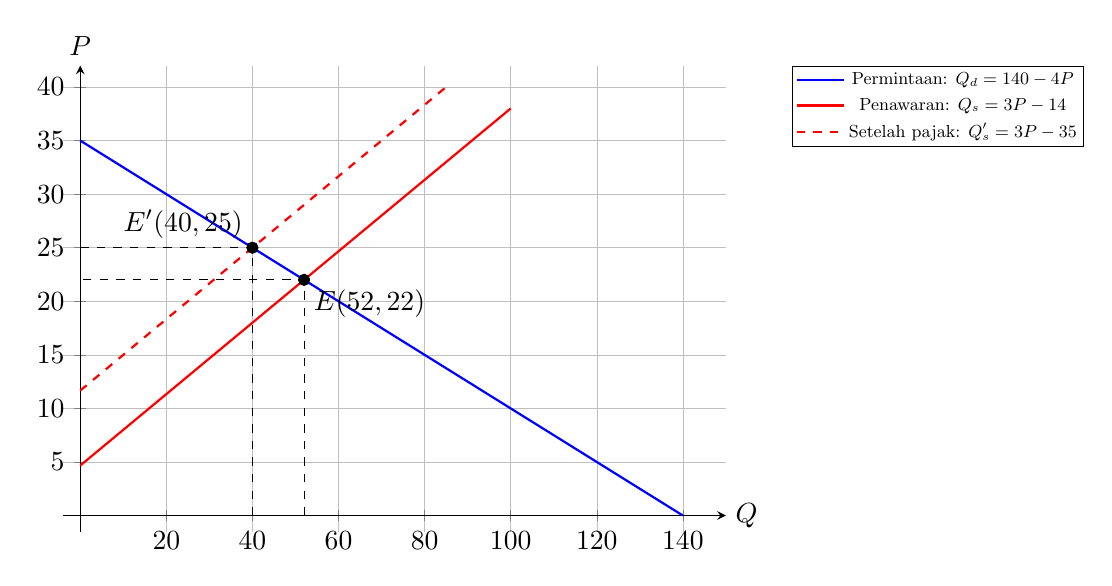
\begin{tikzpicture}
                    \begin{axis}[
        axis lines = middle,
        xlabel = $x$,
        ylabel = {$y$},
        grid=both,
        grid style={line width=.1pt, draw=gray!10},
        major grid style={line width=.2pt,draw=gray!50},
        x label style={anchor=west}, % label x ke kanan
        y label style={anchor=south}, % label y ke atas
        samples=200,
        legend style={
                at={(1.1,1)},
                anchor=north west,
                font=\small,         % mengecilkan ukuran font
                row sep=1pt,         % jarak antar baris legend
                inner sep=1pt,       % margin dalam kotak legend
                nodes={scale=0.7}    % skalakan isi legend
            },
        xlabel = $Q$,
        ylabel = {$P$},
        xtick={0,20,...,140},
        ytick={0,5,...,40},
        xmin=-4, xmax=150,
        ymin=-1.5, ymax=42,
        width=10cm,
        height=7.5cm
    ]
\addplot[domain=0:140, color=blue, thick, samples=2] {(140-x)/4};
\addlegendentry{Permintaan: $Q_d=140-4P$}
\addplot[domain=0:100, color=red, thick, samples=2] {(x+14)/3};
\addlegendentry{Penawaran: $Q_s=3P-14$}
\addplot[domain=0:85, color=red, thick, dashed, samples=2] {(x+35)/3};
\addlegendentry{Setelah pajak: $Q_s'=3P-35$}
\draw[fill=black] (52,22) circle (2pt) node[below right] {$E(52,22)$};
\draw[fill=black] (40,25) circle (2pt) node[above left] {$E'(40,25)$};
\draw[dashed] (52,0) -- (52,22) -- (0,22);
\draw[dashed] (40,0) -- (40,25) -- (0,25);
\end{axis}
                \end{tikzpicture}
            \end{center}
        \end{enumerate}
    }
    \end{jawab}
\end{enumerate}

\newpage

% includepdf hanya dijalankan pada job utama (bukan saat externalize gambar TikZ)
\ifx\pgfactualjobname\tikzexternalrealjob
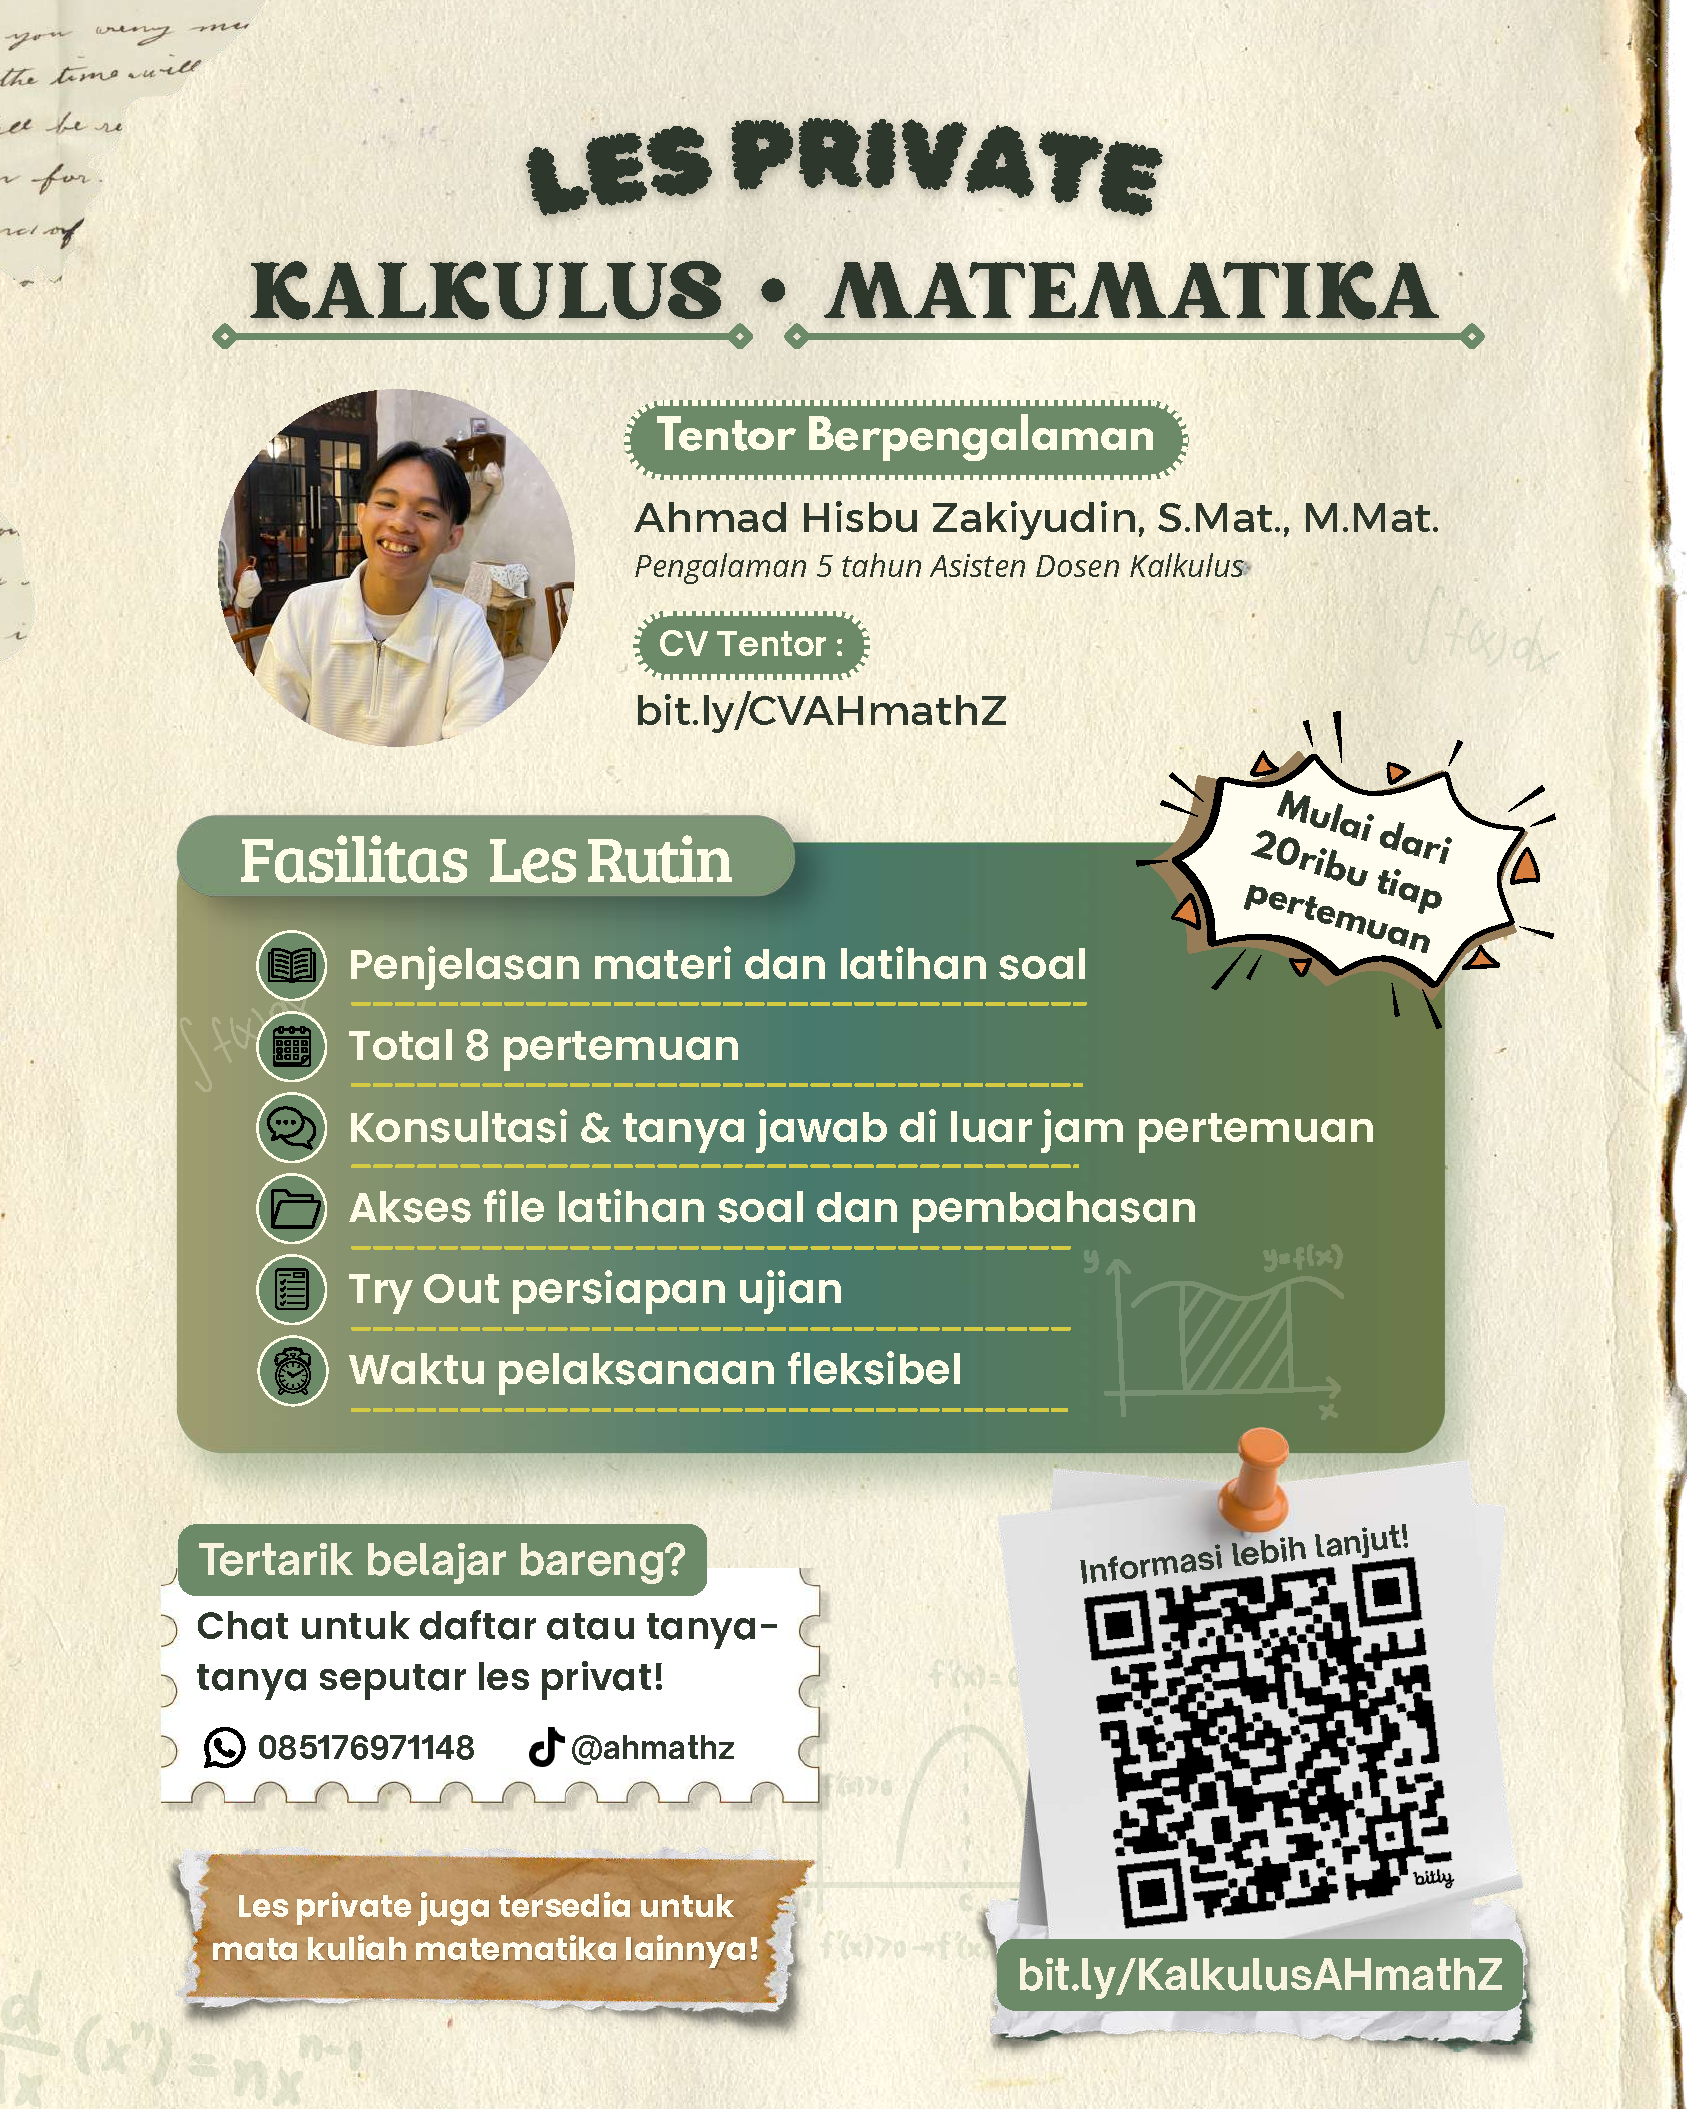
\includepdf[pages=-]{../ETS_Kalkulus_1_Th_2025-2026/les.pdf}
\fi

\end{document}
